\documentclass[11pt,a4paper]{elsarticle} %review=doublespace preprint=single 5p=2 column
%%% Begin My package additions %%%%%%%%%%%%%%%%%%%
\usepackage[hyphens]{url}

  \journal{International Journal of Forecasting} % Sets Journal name


\usepackage{lineno} % add
\providecommand{\tightlist}{%
  \setlength{\itemsep}{0pt}\setlength{\parskip}{0pt}}

\bibliographystyle{elsarticle-harv}
\biboptions{sort&compress} % For natbib
\usepackage{graphicx}
\usepackage{booktabs} % book-quality tables
%%%%%%%%%%%%%%%% end my additions to header

\usepackage[T1]{fontenc}
\usepackage{lmodern}
\usepackage{amssymb,amsmath}
\usepackage{ifxetex,ifluatex}
\usepackage{fixltx2e} % provides \textsubscript
% use upquote if available, for straight quotes in verbatim environments
\IfFileExists{upquote.sty}{\usepackage{upquote}}{}
\ifnum 0\ifxetex 1\fi\ifluatex 1\fi=0 % if pdftex
  \usepackage[utf8]{inputenc}
\else % if luatex or xelatex
  \usepackage{fontspec}
  \ifxetex
    \usepackage{xltxtra,xunicode}
  \fi
  \defaultfontfeatures{Mapping=tex-text,Scale=MatchLowercase}
  \newcommand{\euro}{€}
\fi
% use microtype if available
\IfFileExists{microtype.sty}{\usepackage{microtype}}{}
\usepackage[margin=1.5cm]{geometry}
\ifxetex
  \usepackage[setpagesize=false, % page size defined by xetex
              unicode=false, % unicode breaks when used with xetex
              xetex]{hyperref}
\else
  \usepackage[unicode=true]{hyperref}
\fi
\hypersetup{breaklinks=true,
            bookmarks=true,
            pdfauthor={},
            pdftitle={International Journal of Forecasting 1985-2018: A retrospective based on bibliometric and knowledge diffusion analysis},
            colorlinks=false,
            urlcolor=blue,
            linkcolor=magenta,
            pdfborder={0 0 0}}
\urlstyle{same}  % don't use monospace font for urls

\setcounter{secnumdepth}{5}
% Pandoc toggle for numbering sections (defaults to be off)
% Pandoc header
%% FONT and LAYOUT
\usepackage{mathpazo}
\usepackage{parskip}

%% CAPTIONS
\usepackage{caption}
\DeclareCaptionStyle{italic}[justification=centering]
 {labelfont={bf},textfont={it},labelsep=colon}
\captionsetup[figure]{style=italic,format=hang,singlelinecheck=true}
\captionsetup[table]{style=italic,format=hang,singlelinecheck=true}

%% MATHS
\usepackage{bm}
\allowdisplaybreaks

%% GRAPHICS
\usepackage[section]{placeins}
\setcounter{topnumber}{2}
\setcounter{bottomnumber}{2}
\setcounter{totalnumber}{4}
\renewcommand{\topfraction}{0.85}
\renewcommand{\bottomfraction}{0.85}
\renewcommand{\textfraction}{0.15}
\renewcommand{\floatpagefraction}{0.7}
\usepackage{mathpazo}
\usepackage{parskip}
\usepackage{lscape}
\usepackage{graphicx}
\usepackage{subfigure}
\usepackage{float}
\usepackage{rotating}
\usepackage{rotate}
\usepackage{makecell}
\usepackage{geometry}
\usepackage{indentfirst}



\begin{document}
\begin{frontmatter}

  \title{International Journal of Forecasting 1985-2018: A retrospective based on
bibliometric and knowledge diffusion analysis}
    \author[nau]{Dejian Yu}
   \ead{yudejian62@126.com} 
  
    \author[monash]{Rob J Hyndman}
   \ead{Rob.Hyndman@monash.edu} 
  
    \author[zufe]{Shunshun Shi\corref{c1}}
   \ead{shishunshun1993@126.com} 
   \cortext[c1]{Corresponding Author}
      \address[nau]{Business School, Nanjing Audit University, Nanjing 211815, China}
    \address[monash]{Department of Econometrics \& Business Statistics, Clayton, VIC 3800,
Australia}
    \address[zufe]{Information School, Zhejiang University of Finance and Economics,
Hangzhou 310016, China}
  
  \begin{abstract}
  As one of the leading journals in the forecasting field, International
  Journal of Forecasting (IJF) has continually contributed to the field
  over 30 years. In this study, a retrospective analysis is conducted to
  evaluate the merits of IJF from 1985 to 2018 based on the raw data
  harvested from Scopus. The retrospective analysis consists of two parts.
  One is a bibliometric analysis of IJF based on a science mapping
  technique which focuses on the level of paper, author and country. The
  citation network, co-citation network, co-author network and country
  collaboration network are mapped based on IJF's publications. Multiple
  relationships between different scientific entities can be explored from
  these networks. The other is a knowledge diffusion analysis based on the
  forecasting papers and their citing papers. The discipline distribution
  of citing papers can be obtained with the citation relationship between
  forecasting papers and their citing papers. Besides, a dynamic analysis
  of citing disciplines over time uncovers the changes of knowledge
  diffusion starting from forecasting papers. A deeper investigation about
  the knowledge diffusion outside of the forecasting journals is conducted
  for better elaborating the performance of IJF in knowledge diffusion
  outside the forecasting field. These two kinds of analyses directly
  depict a landscape about the development track of IJF based on the
  endorsements it obtained and the knowledge it spread abroad.
  \end{abstract}
   \begin{keyword} Forecasting research, Bibliometrics, Science mapping, Knowledge
diffusion\end{keyword}
 \end{frontmatter}

\newpage

\section{Introduction}\label{introduction}

\setlength{\parindent}{2em}International journal of forecasting (IJF),
one of the leading journals in the forecasting field, was issued by
International Institute of Forecasters (IIF) in 1985, and then continued
to contribute the forecasting field up to now. According to its website,
the main purpose of the journal is to ``make forecasting useful and
relevant for decision and policy makers'', and all kinds of forecasting
methods are welcomed by the journal for better bridging the gap between
theory and practice. Many of the IJF papers involved the topics in the
fields of business, economics, and management (BEM) for promoting the
forecasting research in these fields. An existing overview about the
forecasting journals which consist of IJF and Journal of Forecasting
(JF) was conducted based on citation analysis and expert opinion, and an
important part of the overview was elaborated under a background of BEM
applications (Fildes 2006). The overview was and remains a valuable
conclusion about the evaluation of the IJF and JF through examining how
they have met their initial objectives successfully, and the content of
the overview is informative. However, the bibliometric techniques which
are used by the overview are sort of simple and not effective enough.
The overview only used one bibliometric technique (i.e., citation
analysis) to analyze the data of IJF, which has left a wide space for
the performance of other bibliometric techniques. Many other overviews
are conducted for evaluating the merits of a certain journal based on
various bibliometric techniques, and a brief summary is provided as
below.

Merigó et al. (2015) conducted an overview of the Journal of Business
Research based on some basic bibliometric techniques, for example,
identifying citation structure, highly cited papers, the most prolific
authors, institutions, and countries. All of them were regarded as the
main factors that affect the performance of the journal, and measured by
the number of publications and citations. Calma and Davies (2016)
provided an overview of Academy of Management Journal using some similar
bibliometric techniques. According to the number of publications the
journal published and citations the journal received, the most prolific
author, countries, organizations, years and highly cited papers, authors
were obtained. Moreover, based on the data of journal papers and their
references, science mapping technique was used to construct the networks
of most prolific authors and most cited authors. Due to the advantage of
delineating relationships between scientific entities, science mapping
has become a frequently-used bibliometric technique for visualizing
different kinds of academic relationships. Wichaisri and Sopadang (2018)
used the data of Sustainable Development to extract the co-citation
relationship between the cited papers, and then determined four main
clusters from the co-citation relationships based on the science mapping
technique.

As stated above, many of the existing overviews have proven the
effectiveness of bibliometric techniques, especially the combination of
basic bibliometric indicators and the science mapping techniques. In our
previous work, this combination has been used in many bibliometric
studies. Our first try of the combination is the study to analyze the
development of Atanassov intuitionistic fuzzy set (Yu and Shi 2015).
Then, this research pattern was successfully applied in aggregation
operator research (Yu 2015). Moreover, an overview of Information
Science (INS) was conducted based on this research pattern to explore
the structures and trends of the INS publications (Yu et al. 2017).
Basically, the majority of the most important factors which affect the
performance of journal can be identified under this research pattern.
Further, some internal relationships between different kinds of
scientific entities can be recognized and expressed by science mapping
techniques. Highly cited paper, author, countries, and prolific author,
country are common factors that can affect the performance of the
journal. Co-citation relationship, co-author relationship, country
collaboration relationship are some common internal relationships
embedded in the journal. The status quo of journal can be elaborated by
these factors and relationships. Moreover, the development track of
journal can be delineated based on a dynamic bibliometric analysis.
However, under this research pattern, the researchis limited inside the
journal, which means the academic activities outside but related to the
journal are difficult to recognize. To settle this problem, the
knowledge diffusion analysis is a good choice.

In bibliometrics, knowledge flow can be constructed based on the citing
and cited behaviors which correspond to the knowledge integration and
knowledge diffusion (Shi et al. 2018), respectively. Knowledge
integration means the knowledge transfer from the cited papers to the
given papers, while knowledge diffusion is from the given papers to the
citing papers. In this study, the raw data of IJF is harvested from
Scopus. However, information about cited papers of IJF publications is
largely missing in Scopus. Therefore, the knowledge integration cannot
be conducted in this study, and we select the knowledge diffusion
analysis as the primary content.

Porter and Chubin (1985) first defined the proportion of citations
falling outside the category as a cross-discipline indicator to
delineate how the knowledge diffuses from the target category to the
outside categories. In Web of Science, the journals are classified based
on the predefined categories, while in Scopus, subject area is used to
replace the concept of category. Therefore, in this study, we use
subject area equaling to the concept of category in the knowledge
diffusion research. IJF and JF are two leading and authoritative
journals in the forecasting field, therefore, IJF papers and JF papers
are all included in the knowledge diffusion analysis. The raw data of
IJF papers, JF papers and their citing papers are harvested from Scopus.
The citation relationships between the IJF papers and their citing
papers are extracted to explore what subject areas are most interested
in the forecasting researches. The same work will be conducted between
JF papers and their citing papers. Then, a rough result about the
knowledge diffusion can be obtained at the level of subject area.
Moreover, to better explore the subject areas that are royal to the
forecasting researches, a dynamic analysis is conducted based on time
slicing. The whole publication time of IJF and JF is divided into three
periods, respectively, and in each period, some typical citing subject
areas which have a special performance in citation behavior are
identified. These typical citing subject areas are selected in a further
investigation and the journal citation relationships between IJF/JF and
their citing journals are extracted. Therefore, more detailed findings
can be obtained at the level of journal. In addition, an overlapping
work is conducted in the typical citing subject areas of IJF and JF. The
derived overlapping subject areas are regarded as the most typical
admirers to the forecasting field. In each subject area, we extract IJF
papers that are cited by more journals belonging to the subject area,
and these papers are most welcomed by the researches outside the
forecasting field. The more journals cite the IJF papers, the more
widely the knowledge of IJF papers spread.

The remainder of this paper is organized as follows. Section 2 presents
a bibliometric analysis of IJF to identify the publication/citation
structure of IJF and the most contributing papers, authors and
countries. Section 3 offers a knowledge diffusion analysis of the
forecasting journals. Section 4 states some discussion and conclusion of
this study.

\section{Bibliometric analysis of
IJF}\label{bibliometric-analysis-of-ijf}

In this section, some frequently-used bibliometric techniques are
applied into analyzing the IJF papers. First, a basic statistics of IJF
papers is provided from the angle of output and citation. Some
interesting findings can be obtained through exploring the relationships
between the curves of annual output and annual citation. Then, paper,
author, and country are selected as the three factors influencing the
performance of the journal. The most cited, co-cited papers, the most
prolific authors, the most cited authors, the most prolific countries,
the most cited countries are all identified. Further, the citation,
co-citation relationships, the co-author relationship, and the country
collaboration relationship are depicted based on science mapping
techniques.

\subsection{Basic statistics of IJF}\label{basic-statistics-of-ijf}

Annual evolutions of papers and citations are depicted in Fig 1, and the
detailed data is stated in the table 1. The Panel A of Fig 1 provides a
view of the overall trend to analyze the dynamic of papers and
citations. Observing from the paper curve, there is a decrease of the
yearly output from 1996 to 2001, but, by the large, the yearly output
increased over time. The most prolific year is 2016 with 105 papers, and
the least productive year is the initial year with 27 papers. As for the
annual evolution of citations, the situation is similar to that of
paper. By the large, the number of citations increased over time, but
with a little drop in the period of 1996-2001. The number of citations
in the year of 2006 is the highest, which largely owes to a highly cited
paper (i.e., received 1198 citations) written by (Hyndman and Koehler
2006). After the year of 2006, the number of citations had a wavy
decrease. In addition, the shape of citation curve is quite similar to
that of paper curve, especially the periods of 1984-1994 and 2010-2018.

To deeply investigate the relation between the citation curve and the
paper curve, these two curves are divided into four pieces in the Panel
B, C, D, and E. In the Panel B and E, the trends of paper and citation
are quite similar, which is reflected in every peak point and valley
point. However, the interspace between the paper curve and citation
curve is bigger in the Panel E than in the Panel B, which indicates the
ratio of citations per paper is dropping from the initial years to the
latest years. This phenomenon may result from two reasons. One is the
increased academic output around the world. Another is the shorter
citation time window, which means the papers published in the latest
years do not have enough time to accumulate their citations.

In the Panel C, the shapes of paper curve and citation curve are still
kind of similar, but the ratio of citations per paper from 1997 to 2000
is much higher than the remaining years, which indicates the papers
published in 1997, 1998, 1999 and 2000 attracted more citations than
others. To better investigate why these papers can attract more
citations, we have a closer look at the raw data of these papers, and we
find each year has one or two highly cited papers. A highly cited paper
with 564 citations was published in 1997, and focused on testing the
equality of prediction mean squared errors (D. Harvey, Leybourne, and
Newbold 1997). In 1998, Zhang et al. proposed to investigate the effect
of key factor on forecasting performance of artificial neural network
(Zhang, Patuwo, and Hu 1998), and this research has accumulated 2007
citations. In 1999, a research analyzing the Delphi technique as a
forecasting tool was conducted (Rowe and Wright 1999), and received 941
citations. In 2000, Makridakis and Hibon (2000) describes a
M3-Competition, and compare the results of the latest M3-Competition
with previous M-Competitions. The research of Makridakis and Hibon
received 669 citations. Based on the raw data from 1985 to 2018
harvested from Scopus, only eight papers have more 500 citations, and
four of eight occurred in the period of the Panel C. In the Panel D,
there is a peak point during the whole citation curve which is the year
of 2006, and there are eight papers received more 100 citations in 2006.
Among these papers, the study conducted by Hyndman and Koehler (2006) is
the most highly cited with 1198 citations, which contributes to one
fourth of the total citations in 2006.

\begin{figure}[htbp]
\centering
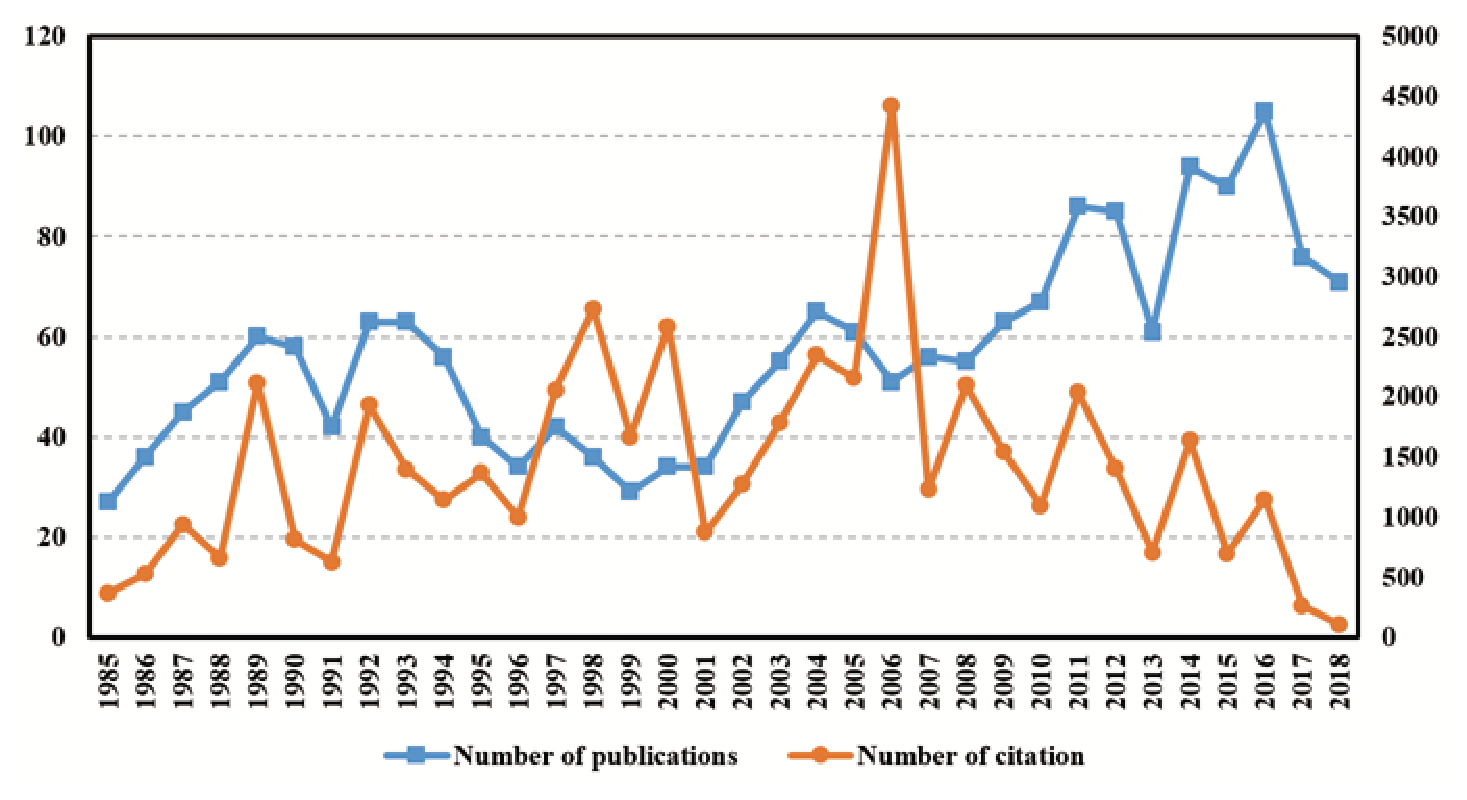
\includegraphics[scale=0.4]{fig.1.eps}
\caption{Annual evolutions of IJF papers and citations from 1985 to 2018}
\end{figure}\newpage

\subsection{Citation network and co-citation
network}\label{citation-network-and-co-citation-network}

After an overall review about the total IJF papers from 1985 to 2018, we
focus on evaluating the performance of single IJF paper. The top 20 most
cited IJF papers are listed in table 1 with the information about the
citation number, author names, publication year, etc. Note that the
country in table 1 refers to the country of first author and UK contains
England, Scotland, Walsh, and North Ireland. The top three most cited
papers all receive over 1000 citations, and the first one even possesses
over 2000 citations. These three papers already appear in the subsection
2.1 as the important contributors for promoting the citations of their
publication years. The first one is the paper written by Zhang, Patuwo,
and Hu (1998) which investigated the research on forecasting with
artificial neural networks. The second is the work of Hyndman and
Koehler (2006) which considered the mean absolute scaled error as the
standard measure based on comparing the accuracy of multiple forecasting
methods. The third is Clemen (1989) which provided a review about the
research on forecast combination and suggestions for the future work.

\begin{table}[!htbp]
\centering
\caption{Information about top 20 most cited IJF papers}
\setlength{\tabcolsep}{4mm}{
\begin{tabular}{ccccccc}
\hline
Rank & Paper & TC & TC/Year & Country & Nau & Nin\\
\hline
1 & Zhang et al. (1998) & 2007 & 95.57 & USA & 3 & 1\\
2 & Hyndman and Koehler (2006) & 1198 & 92.15 & Australia & 2 & 2\\
3 & Clemen (1989) & 1105 & 36.83 & USA & 1 & 1\\
4 & Rowe and Wright (1999) & 941 & 47.05 & UK & 2 & 2\\
5 & Makridakis and Hibon (2000) & 669 & 35.21 & France & 2 & 1\\
6 & De Gooijer and Hyndman (2006) & 612 & 47.08 & Netherlands & 2 & 2\\
7 & Armstrong and Collopy (1992) & 573 & 21.22 & USA & 2 & 2\\
8 & Harvey et al. (1997) & 564 & 25.64 & UK & 3 & 1\\
9 & Witt and Witt (1995) & 468 & 19.50 & UK & 2 & 2\\
10 & Thomas (2000) & 390 & 20.53 & UK & 1 & 1\\
11 & Meade and Islam (2006) & 381 & 29.31 & UK & 2 & 2\\
12 & Gardner (2006) & 377 & 29.00 & USA & 1 & 1\\
13 & Diebold and Yilmaz (2012) & 375 & 53.57 & USA & 2 & 3\\
14 & Holt (2004) & 372 & 24.80 & USA & 1 & 1\\
15 & Weron (2014) & 345 & 69.00 & Poland & 1 & 1\\
16 & Hyndman et al. (2002) & 310 & 18.24 & Australia & 4 & 2\\
17 & Conejo et al, (2005) & 282 & 20.14 & Spain & 4 & 2\\
18 & Taylor et al., (2006) & 265 & 20.38 & UK & 3 & 3\\
19 & Brown (1993) & 221 & 8.50 & USA & 1 & 1\\
20 & Lawrence (2006) & 212 & 16.31 & Australia & 4 & 4\\
\hline
\end{tabular}}
\end{table}

Besides, a citation network is mapped based on the citation relationship
between IJF papers. The citation network consists of nodes and links,
where some nodes are connected with links and some are isolated. A node
represents a paper and a link represents the citation relationship
between any two connected papers. The size of node is denoted as the
number of citations a paper received. Through this citation network, the
citation relationships between any connected IJF papers can be visually
obtained and deeper investigations like highly cited publications are
cited by what papers can be conducted easily. The number of citations no
less than 80 is set as the limitation, then 111 qualified IJF papers are
derived. 29 of the 111 papers are discarded because they are isolated.
Finally, 82 IJF papers are used to construct this citation map, as shown
in Fig. 2. Distance between any pair of papers denotes their similarity
calculated by the association strength method (Eck and Waltman 2009) The
longer distance is the more dissimilar the two connected papers are.
Papers with high similarity values are clustered and represented as the
same color. Among the 82 IJF papers, 70 of them have citations, while
the remaining 12 papers have no citations, but cite to some of the 70
papers. From Fig. 2, Zhang, Patuwo, and Hu (1998) is the biggest node
because it is the most cited paper among the total IJF papers, but among
these 82 IJF papers, it is not the paper that has the most citations
from the 82 IJF papers. The 82 IJF papers in Fig. 2 are all highly cited
papers, so their endorsements are pretty authoritative. Winning an
endorsement from these 82 papers helps a lot to promote the prestige of
the paper, so a further investigation is conducted to derive the highly
cited papers, where their citations are from these 82 papers. We define
the citation from the IJF papers as the local citation (LC). The papers
having no less than 5 local citations are extracted, as shown in table
2. Paper written by Gooijer and Hyndman (2006) is the most cited among
these 82 IJF papers, and the paper is about a 25 review on time series
forecasting based on the papers of JIF and Journal of Forecasting (JF).
According to the local citation percentage (LC/TC), the research of
Crone, Hibon, and Nikolopoulos (2011) ranks the first, which indicates
the high quality of its citations. Zhang, Patuwo, and Hu (1998) is top
one highly cited in the total IJF papers, but its performance in local
citation percentage is not that remarkable.

\begin{figure}[htbp]
\centering
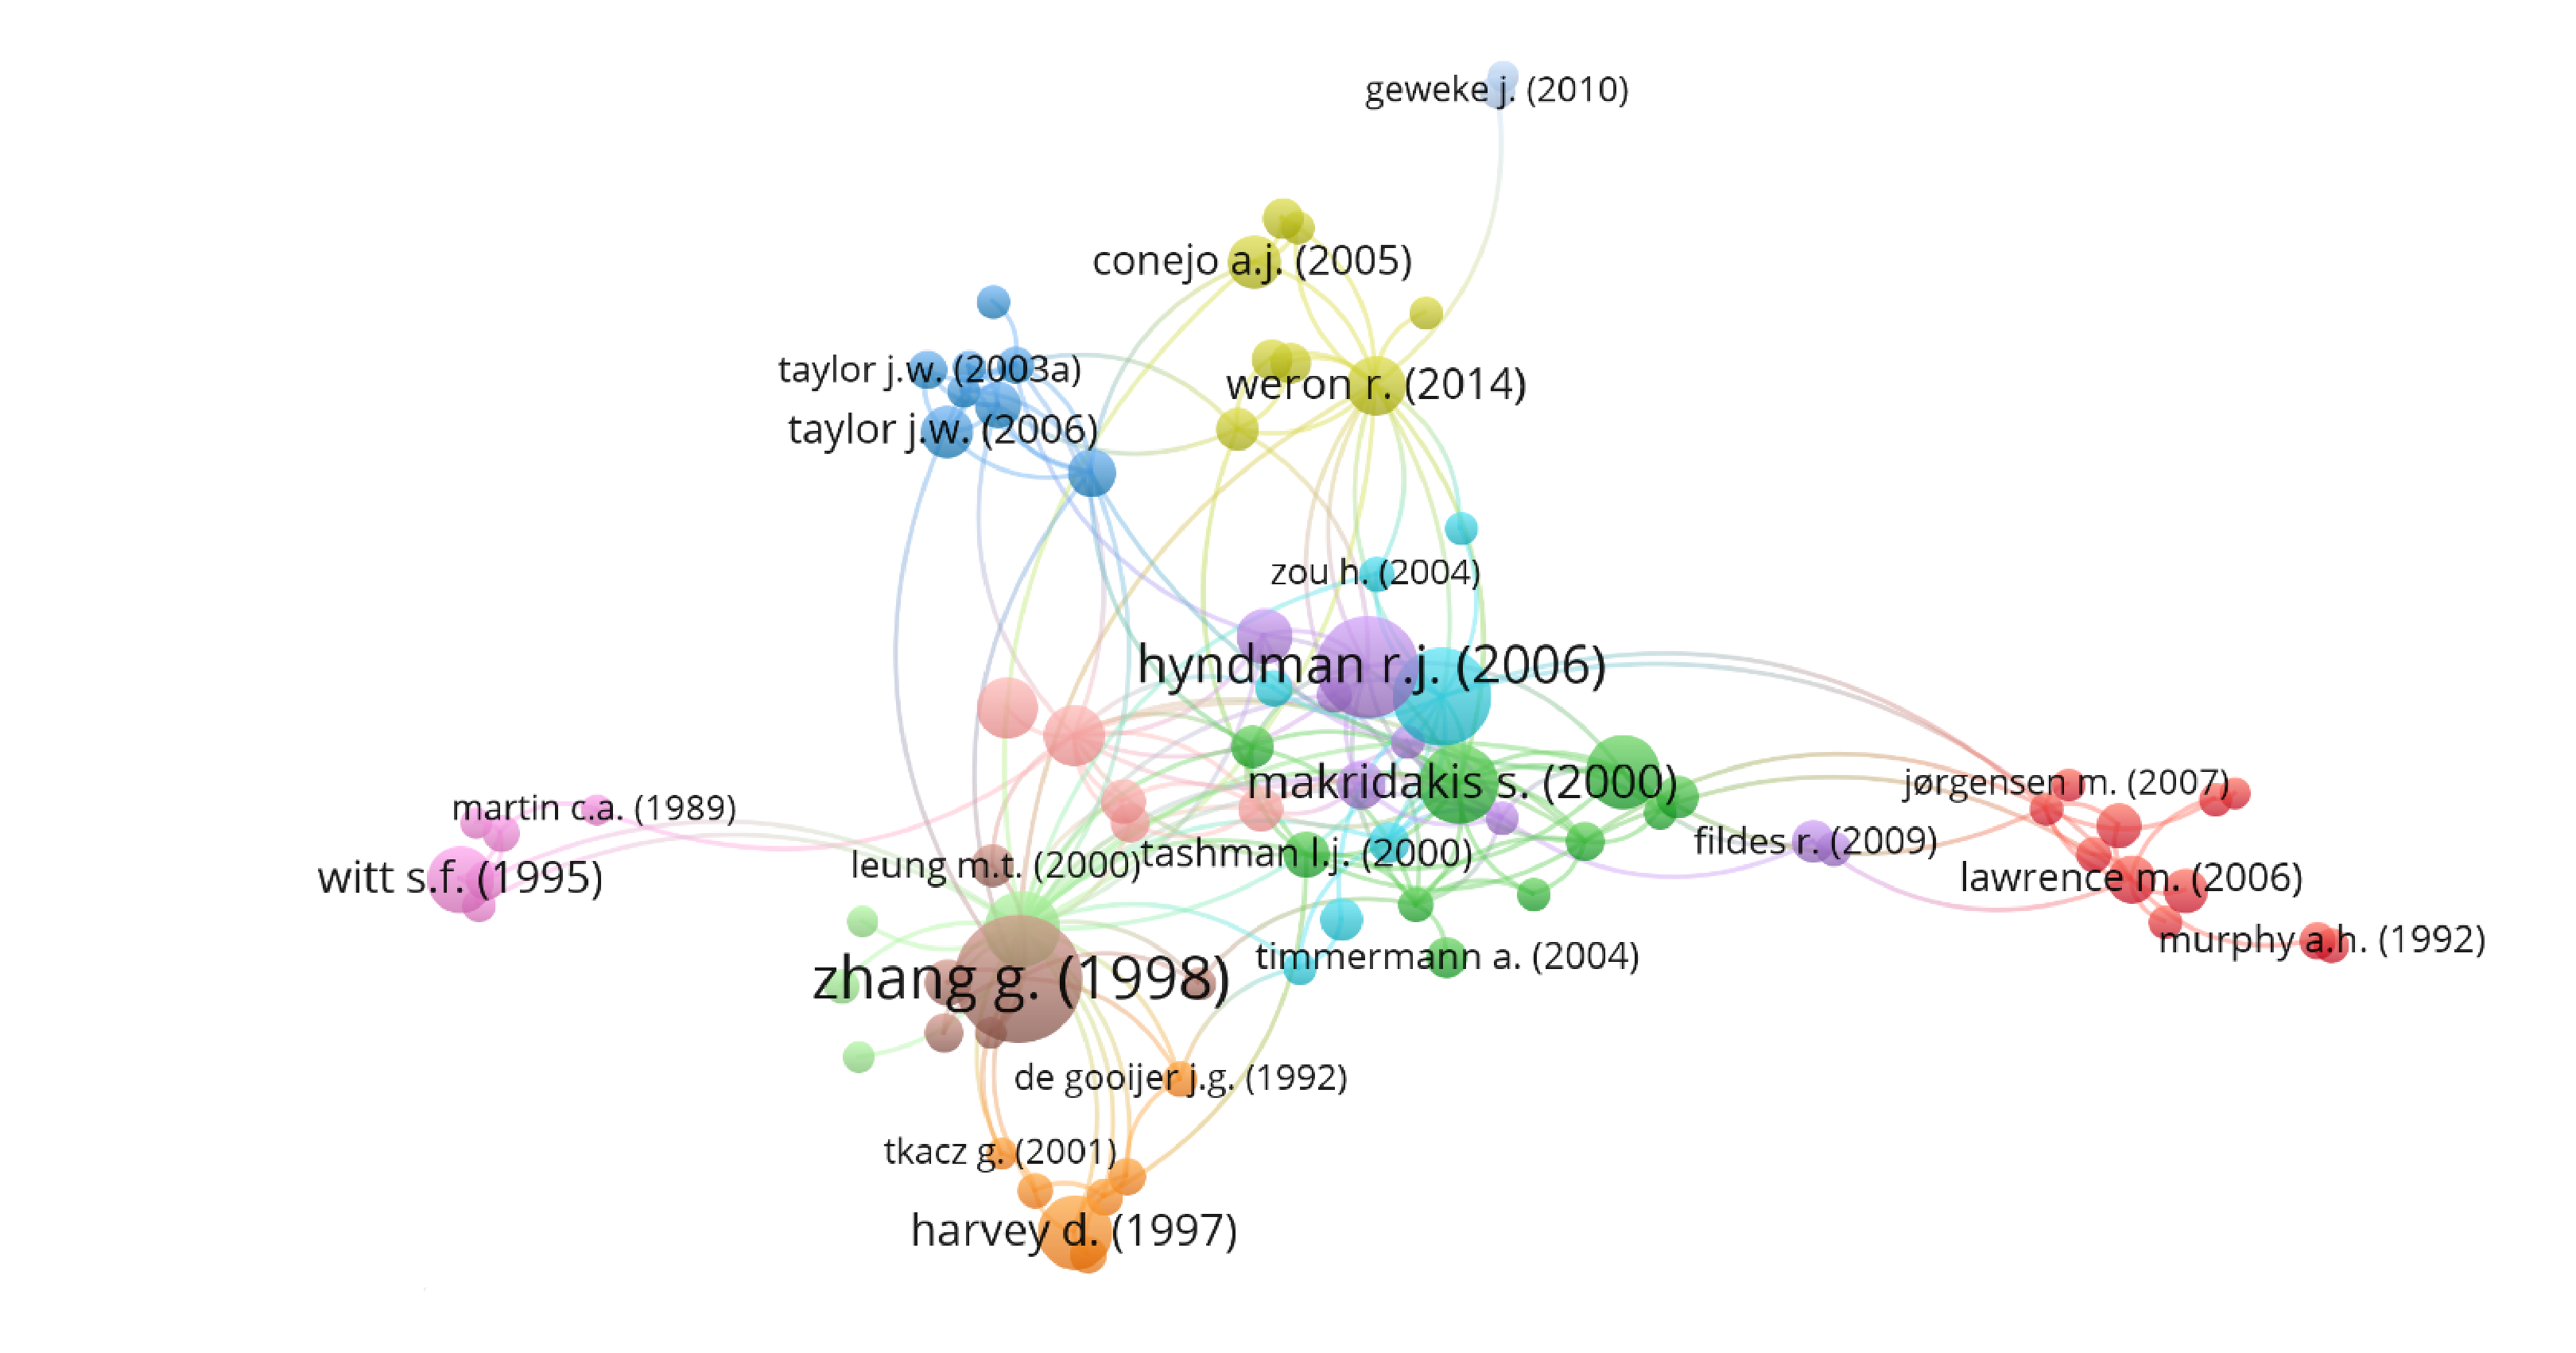
\includegraphics[width=16cm,height=9cm]{fig.2.eps}
\caption{Citation network of 82 most cited IJF papers}
\end{figure}

\begin{table}[!htbp]
\centering
\caption{Information about the most local cited IJF papers}
\setlength{\tabcolsep}{8.7mm}{
\begin{tabular}{ccccc}
\hline
Rank & Paper & LC & TC & LC/ TC\\
\hline
1 & De Gooijer and Hyndman (2006) & 33 & 612 & 5.39\%\\
2 & Weron (2014) & 17 & 345 & 4.93\%\\
3 & Gardner (2006) & 16 & 377 & 4.24\%\\
4 & Makridakis and Hibon (2000) & 16 & 669 & 2.39\%\\
5 & Zhang et al. (1998) & 12 & 2007 & 0.60\%\\
6 & Clemen (1989) & 11 & 1105 & 1.00\%\\
7 & Crone et al. (2011) & 10 & 108 & 9.26\%\\
8 & Taylor et al. (2008) & 10 & 124 & 8.06\%\\
9 & Lawrence et al. (2006) & 10 & 212 & 4.72\%\\
10 & Darbellay and Slama (2000) & 10 & 207 & 4.83\%\\
11 & Makridakis (1993) & 10 & 133 & 7.52\%\\
\hline
\end{tabular}}
\end{table}

Co-citation analysis is one of the useful bibliometric methods. As the
name suggested, the co-citation relationship describes the relations
between any two co-cited papers, and the co-cited papers means papers
that are cited by the same paper. If two papers are cited by one same
paper, then these two papers are in a co-citation relationship and the
co-citation strength they possess is one. Based on the IJF papers
harvested from Scopus, the co-citation relationships between them and
citing papers are extracted. Note that 122 IJF papers are excluded
because of the missing data and format errors. Finally, 1816 IJF papers
and 33204 references are included in this co-citation network, shown in
Fig. 3. IJF papers published in the same year are divided into one group
to better straighten out their co-citation evolution trajectory.
Moreover, three groups of thresholding are used to control the
filtration of the qualified papers. Each group of thresholding has three
criterion which are the minimum citations, minimum co-citations, and
minimum normalized co-citations. The first thresholding is set in the
year of 1985, the second in 2002, and the last is in 2018. After some
trail runs, the first thresholding is set with 50, 3, 15, the second is
3, 3, 20, and the third is 3, 3, 20.

\begin{figure}[!htbp]
\centering
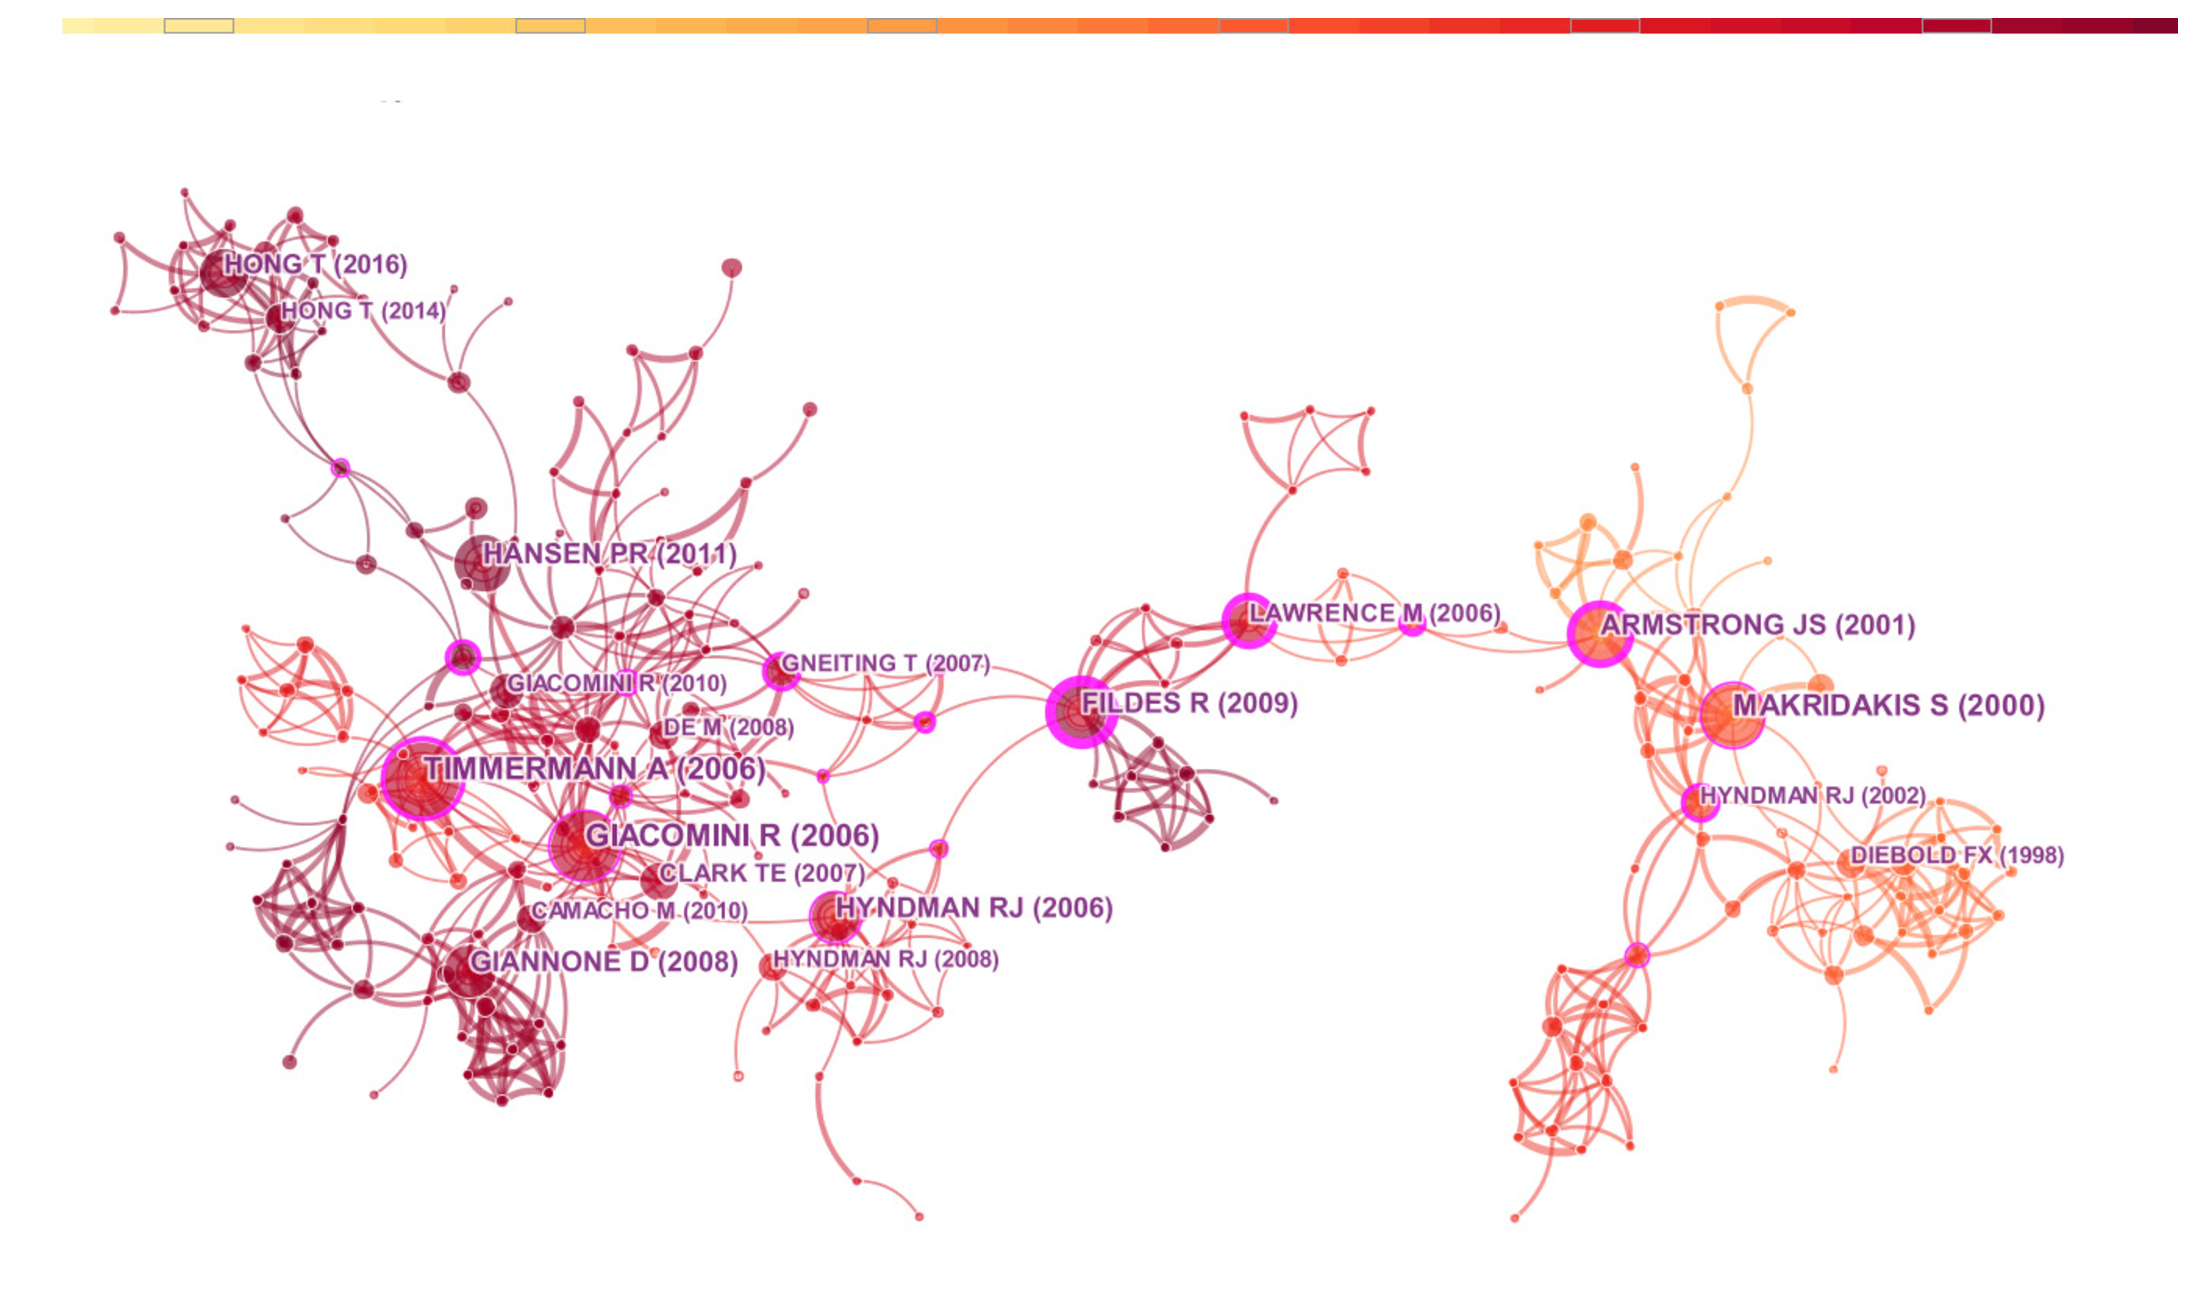
\includegraphics[scale=0.4]{fig.3.eps}
\caption{Co-citation network of IJF papers and their citing papers}
\end{figure}

The color in the Fig. 3 denotes the publication year of papers, and the
warm color represents the latest year, while the cold color represents
the old year. The size of node denotes the co-cited times of each paper,
and the bigger the size is the more the co-cited times are. From Fig. 3,
we can see that the coldest color is green (i.e., approximately
corresponds to the year of 1998), which means the papers published
earlier are excluded according to the thresholding. The top 10 most
co-cited papers which have the biggest nodes are extracted and listed in
table 3. The most co-cited research conducted by Timmermann (2006)
elaborated on the advantages of forecast combination, and analyzed the
factors that can determine the advantages. The second most co-cited work
(Giannone, Reichlin, and Small 2008) provided a framework which was
useful for the real-time forecast selection based on conditional
expectations of forecasts, and applied this framework into a testing
problem. The third most co-cited work is an IJF paper written by
Makridakis and Hibon (2000) which described a M3-Competition. This IJF
paper also is the main contributor for the high citations in the year of
2000. Including the work of Makridakis and Hibon (2000), we find that
four of the ten most co-cited papers are IJF papers, which means these
four IJF papers possess the most co-endorsements from IJF papers. In
table 3, except for the co-citation, the information about the first
co-cited year, the last co-cited year, the whole co-cited duration, and
the average co-citation per year about each top ten co-cited papers are
provided. Among these four IJF papers, we find the research conducted by
Hong et al. (2016) has the shortest co-cited duration, but the highest
average co-citation per year, which denotes the research (Hong et al.
2016) is very frequently co-cited by others in recent years. From the
Fig. 3, we can see the study (Hong et al. 2016) is in a co-citation
relationship with his another research (Hong, Pinson, and Fan 2014), and
these two researches are both related to the energy forecasting. Another
two IJF papers are the work of Hyndman and Koehler (2006) and the work
of Fildes et al. (2009) which both possess relatively low average
co-citation per year, and it denotes they are behind Hong's work (Hong
et al. 2016) in co-cited activity. One thing is interesting that the
node of Fildes et al. (2009) is wrapped with a purple ring in Fig. 3,
where the purple ring means the node enjoys a high between-ness
centrality. The between-ness was proposed by Freeman (1977) and depicts
the structural property of communication of nodes between connected
networks. A node with high between-ness centrality denotes it is more
inclined to be positioned between some connected networks. In Fig. 3,
the node of Fildes et al. (2009) is between a red cluster and a yellow
cluster, which means the node of Fildes et al. (2009) linked the
researches published earlier than 2009 and later than 2009. Fildes et
al. (2009) plays an important role in expressing the connected
co-citation relationships between these two clusters of researches.
Besides, another work called burst detection is conducted to identify
papers with abrupt change (Kleinberg 2003), as shown in Fig. 4. The
papers with abrupt change usually are the milestone papers of the
science mapping research. From Fig. 4, we can find that the same four
IJF papers having high co-citations are also remarkable in this burst
detection, especially, the work of Makridakis (Makridakis and Hibon
2000) has the strongest burst power, which means it is the most
important milestone in this co-citation mapping.

\begin{figure}[htbp]
\centering
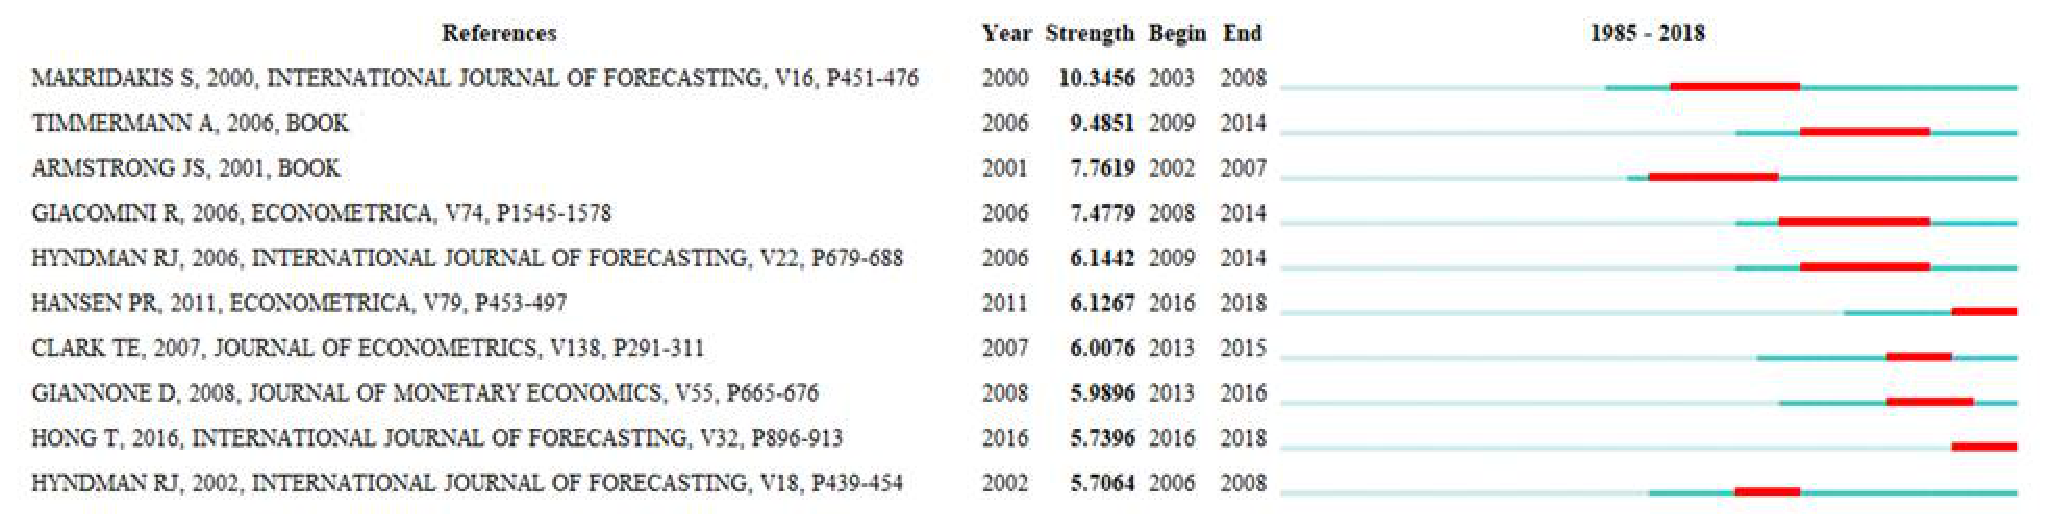
\includegraphics[scale=0.5]{fig.4.eps}
\caption{Papers with the strongest power in the burst detection. }
\end{figure}

\begin{landscape}
\begin{table}[!htbp]
\caption{Information about the most co-cited papers in the co-citation network}
\newcommand{\tabincell}[2]{\begin{tabular}{@{}#1@{}}#2\end{tabular}}
\setlength{\tabcolsep}{2.2mm}{
\begin{tabular}{c c c c c c c c c c}
\hline
Rank & Co & Paper & Source &    FY &    LY &    Y & best year (number) &    Ave-Co &    Citation\\
\hline
1 & 26 & Timmermann (2006) & Handbook of economic forecasting & 2009 & 2014 & 6 & 2009(9) & 4.33 & 1247\\
2 & 24 & Giacomini and White (2006) & Econometrica & 2007 & 2014 & 8 & 2009/2011/2013(5) & 3.00 & 1231\\
3 & 22 & Makridakis and Hibon (2000) & International journal of forecasting & 2003 & 2008 & 6 & 2006(7) & 3.67 & 1325\\
4 & 20 & Hansen et al. (2011) & Econometrica & 2012 & 2018 & 7 & 2018(7) & 2.86 & 1036\\
5 & 18 & Giannone et al. (2008) & Journal of Monetary Economics & 2013 & 2018 & 6 & 2016(8) & 3.00 & 793\\
6 & 17 & Hyndman and Koehler (2006) & International journal of forecasting & 2009 & 2014 & 6 & 2011(6) & 2.83 & 2338\\
7 & 16 & Armstrong (2001) & \tabincell{c}{Principles of Forecasting: \\ A Handbook for Researchers and Practitioners} & 2001 & 2007 & 7 & 2002/2006(6) & 2.28 & 1740\\
8 & 15 & Fildes et al. (2009) & International journal of forecasting & 2011 & 2017 & 7 & 2013(7) & 2.14 & 299\\
9 & 14 & Hong et al. (2016) & International journal of forecasting & 2016 & 2018 & 3 & 2016(8) & 4.67 & 251\\
10 & 14 & Lawrence (2006) & Journal of the American College of Cardiology & 2007 & 2013 & 7 & 2013(6) & 2.00 & 379\\
\hline
\end{tabular}}
\end{table}
\end{landscape}

\newpage

\subsection{Authors analysis in IJF and co-author
network}\label{authors-analysis-in-ijf-and-co-author-network}

Prolific authors can be regarded as the experts of the field or the
important contributors of the journal. After a preliminary review, some
prolific associate editors who published in IJF are excluded because the
researches of associate editors are more inclined to be highly cited
than those of normal IJF authors. The top ten prolific authors in IJF
are selected from the remaining IJF authors, as shown in table 4. The
information about their first paper year, and last paper year is stated
in table 4. We find that most of the ten prolific authors possess a long
academic career, especially Koehler and Ord whose papers covering at
least 30 years. Five of the ten authors affiliated in USA, which
indicates the USA scholars form a leading and active community in IJF.
Generally speaking, first author is the main contributor of a paper, and
corresponding author is responsible for a paper. Therefore, we calculate
the number of papers that the authors are responsible for the first
authors or the corresponding authors. From table 4, Chatfield's first
author percentage is 86.67\% which is the highest among the ten authors,
followed by Taylor and Lahiri. O'Connor and Ord are two authors who have
relatively weak performance in first author percentage and corresponding
author percentage. It means that they are prolific authors in IJF, but
in most cases, they acted as a collaborator of the papers, rather than
the main contributor.

\begin{table}[!htbp]
\centering
\caption{Information about the top ten prolific authors in IJF}
\setlength{\tabcolsep}{3mm}{
\begin{tabular}{ccccccccccc}
\hline
Rank & Author & TP & Country & FY & LY & Y & 1st & 1st \% & Cor & Cor \%\\
\hline
1 & Franses, P. H. & 26 & Netherlands & 1991 & 2017 & 27 & 12 & 46\% & 13 & 50\%\\
2 & Stekler, H. O. & 24 & USA & 1988 & 2015 & 28 & 10 & 42\% & 12 & 50\%\\
3 & Goodwin, P. & 22 & UK & 1993 & 2017 & 25 & 10 & 45\% & 13 & 59\%\\
4 & Koehler, A.B. & 19 & USA & 1985 & 2017 & 33 & 6 & 32\% & 10 & 53\%\\
5 & O'Connor, M. & 18 & Australia & 1989 & 2007 & 19 & 5 & 28\% & 7 & 39\%\\
6 & Taylor J.W. & 16 & UK & 1999 & 2018 & 20 & 13 & 81.25\% & 14 & 87.50\%\\
7 & Lawrence M. & 15 & Australia & 1992 & 2011 & 20 & 7 & 46.67\% & 6 & 40.00\%\\
8 & Ord & 15 & USA & 1988 & 2017 & 30 & 4 & 26.67\% & 5 & 33.33\%\\
9 & Chatfield C. & 15 & USA & 1986 & 1995 & 10 & 13 & 86.67\% & 10 & 66.67\%\\
10 & Lahiri K. & 15 & USA & 1987 & 2015 & 29 & 12 & 80.00\% & 9 & 60.00\%\\
\hline
\end{tabular}}
\end{table}

The number of citations an author received is a useful indicator to
evaluate the prestige of authors, therefore, the top ten most cited
authors are selected in table 5. Similar to the table 4, the associate
editors are excluded in table 5. Koehler is the most cited author due to
his relatively high output. Wright has the highest TC/TP value, which is
largely due to his highly cited paper, ``The Delphi technique as a
forecasting tool: Issues and analysis'' (Rowe and Wright 1999). Franses
is the most prolific author, but ranks the last in TC, which indicates
his researches are not as attractive as those of the other nine authors.
Besides, the number of citations from the IJF and outside the IJF are
calculated. Goodwin, Collopy, Hibon and O'Connor receive higher local
citation percentage, which means the IJF endorsements their researches
obtained are more than those of the remaining authors.

\begin{table}[!htbp]
\centering
\caption{Information about the top ten most cited IJF authors}
\setlength{\tabcolsep}{3.5mm}{
\begin{tabular}{cccccccccc}
\hline
Rank & Author & TC & TP & RTP & TC/TP & LC & \% & OC & \%\\
\hline
1 & Koehler, A.B. & 1634 & 19 & 3 & 86 & 79 & 4.83\% & 1555 & 95.17\%\\
2 & Wright, G. & 1180 & 9 & 8 & 131.11 & 47 & 3.98\% & 1133 & 96.02\%\\
3 & Hibon, M. & 1016 & 11 & 6 & 92.36 & 131 & 12.89\% & 885 & 87.11\%\\
4 & Taylor J.W. & 750 & 16 & 5 & 46.88 & 33 & 4.40\% & 717 & 95.60\%\\
5 & De Gooijer, J.G. & 738 & 9 & 9 & 82.00 & 31 & 4.20\% & 707 & 95.80\%\\
6 & Collopy, F. & 675 & 12 & 10 & 56.25 & 96 & 14.22\% & 579 & 85.78\%\\
7 & Franses, P. H. & 665 & 26 & 1 & 25.58 & 57 & 8.57\% & 608 & 91.43\%\\
8 & Goodwin, P. & 656 & 22 & 2 & 29.82 & 95 & 14.48\% & 561 & 85.52\%\\
9 & O’Connor, M. & 653 & 18 & 4 & 36.28 & 84 & 12.86\% & 569 & 87.14\%\\
10 & Meade, N. & 598 & 10 & 7 & 59.80 & 31 & 5.18\% & 567 & 94.82\%\\
\hline
\end{tabular}}
\end{table}

A co-author network is constructed based on the co-author relationship
between IJF authors. Authors who publish less than eight papers are
discarded, then 38 qualified authors are derived. Among the 38 authors,
6 authors are isolated, so finally 32 authors are mapped into the
co-author network, as shown in Fig.5.

\begin{figure}[htbp]
\centering
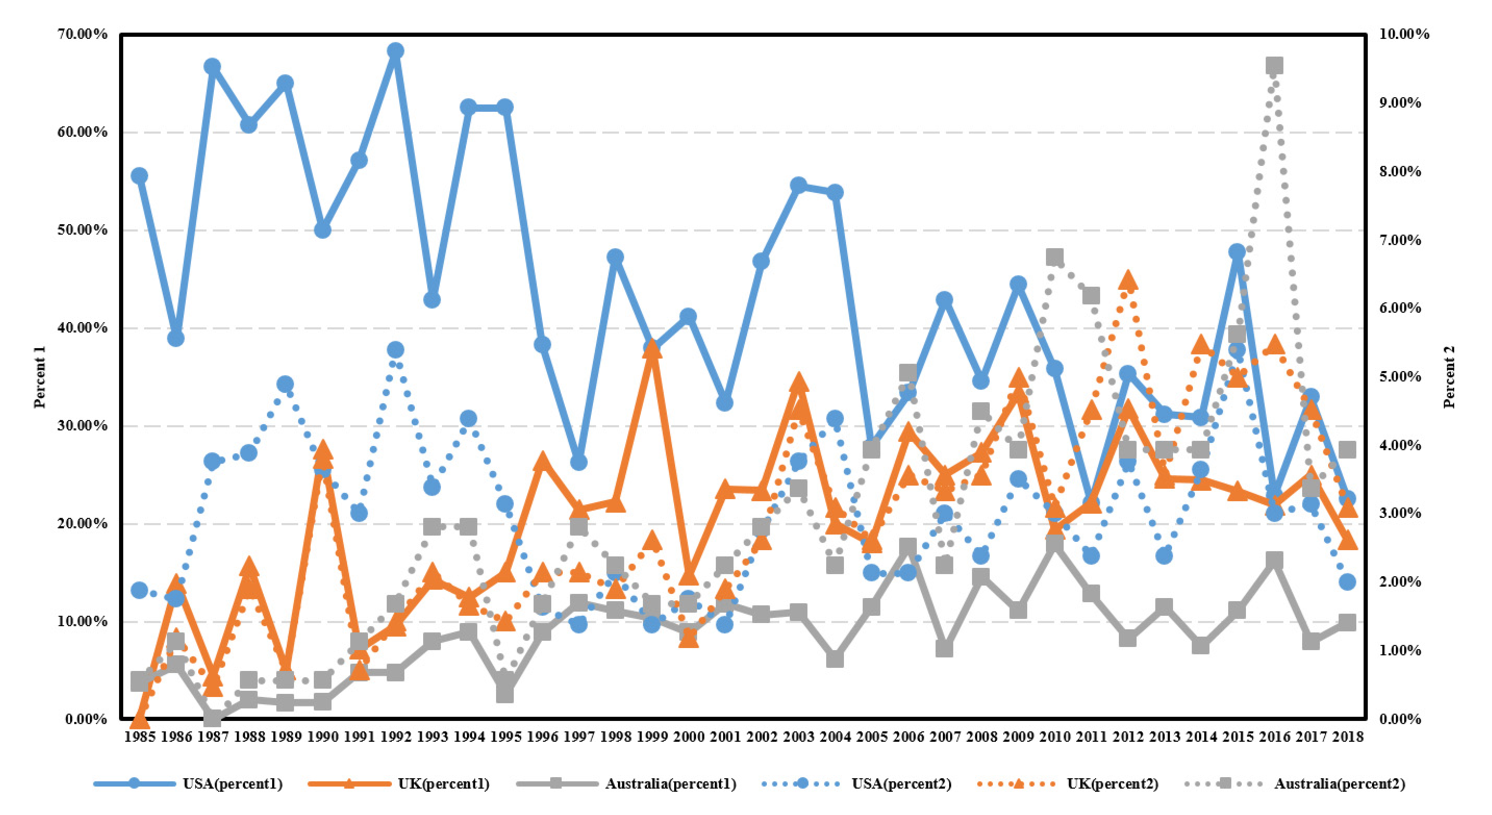
\includegraphics[scale=0.4]{fig.5.eps}
\caption{Co-author network of the most prolific IJF authors}
\end{figure}

\subsection{Country analysis and country co-occurrence
network}\label{country-analysis-and-country-co-occurrence-network}

In this subsection, we extract some prolific countries and most
attractive countries according to the number of publications and
citations. Based on this analysis, we can identify what countries are
the biggest providers of IJF and what countries possess the highest
authority in IJF. Besides, a country co-occurrence network is provided
to express the collaboration relationships among different countries.

Country is a geographical community producing the academic researches,
and the large academic output of a country declares the high academic
productivity of the country. Therefore, country is selected as the
objective of this subsection, and analyzed based on the number of papers
each country produced and the number of citations they received.
Information about the top ten prolific countries are listed in table 6.
USA, UK, and Australia rank the top places, and their durations range
the whole issue period of IJF. USA is the dominant country whose papers
occupy around 41\% of the total IJF papers. Moreover, most of the
prolific countries belong to Europe and North America, which indicates
the developed countries in Europe and North America are still the main
producers of IJF papers. Besides, a dynamic analysis is conducted based
on the output of these ten countries, and the whole period (i.e., years
from 1985 to 2018) is divided into three slices, as shown in Fig. 6. The
left chart of the Fig. 6 depicts the percentage dynamic in the same
country based on three time slices, while the right chart of the Fig. 6
provides the dynamic of each prolific country's percentage of the total
IJF papers in three time slices. From the left chart, the percentage
change of USA is not obvious, and the same as that of Canada. Except for
USA and Canada, the percentages of the remaining countries have
increased greatly over time, which indicating the forecasting researches
is growing fast in these countries. From the right chart, USA is in the
dominant position, as the most productive country in IJF. However, the
percentage it possess is decreasing over time, which means it is losing
its output advantage in IJF as the production rises in other countries.
UK, Australia, and Germany are showing signs of active productivity.

\begin{table}
\centering
\caption{Information about the top ten prolific countries}
\setlength{\tabcolsep}{6mm}{
\begin{tabular}{cccccccc}
\hline
Rank & Country & TP & FY & LY & Y & TP/Y & \% of total\\
\hline
1 & USA & 798 & 1985 & 2018 & 34 & 23.47 & 41.18\%\\
2 & UK & 420 & 1985 & 2018 & 34 & 12.35 & 21.67\%\\
3 & Australia & 178 & 1985 & 2018 & 34 & 5.24 & 9.18\%\\
4 & Germany & 110 & 1988 & 2018 & 31 & 3.55 & 5.68\%\\
5 & Netherlands & 99 & 1988 & 2018 & 31 & 3.19 & 5.11\%\\
6 & Spain & 93 & 1986 & 2018 & 33 & 2.82 & 4.80\%\\
7 & Canada & 84 & 1985 & 2018 & 34 & 2.47 & 4.33\%\\
8 & Italy & 70 & 1987 & 2018 & 32 & 2.19 & 3.61\%\\
9 & France & 67 & 1986 & 2018 & 33 & 2.03 & 3.46\%\\
10 & Belgium & 36 & 1989 & 2018 & 30 & 1.20 & 1.86\%\\
\hline
\end{tabular}}
\end{table}

\begin{figure}[htbp]
\centering
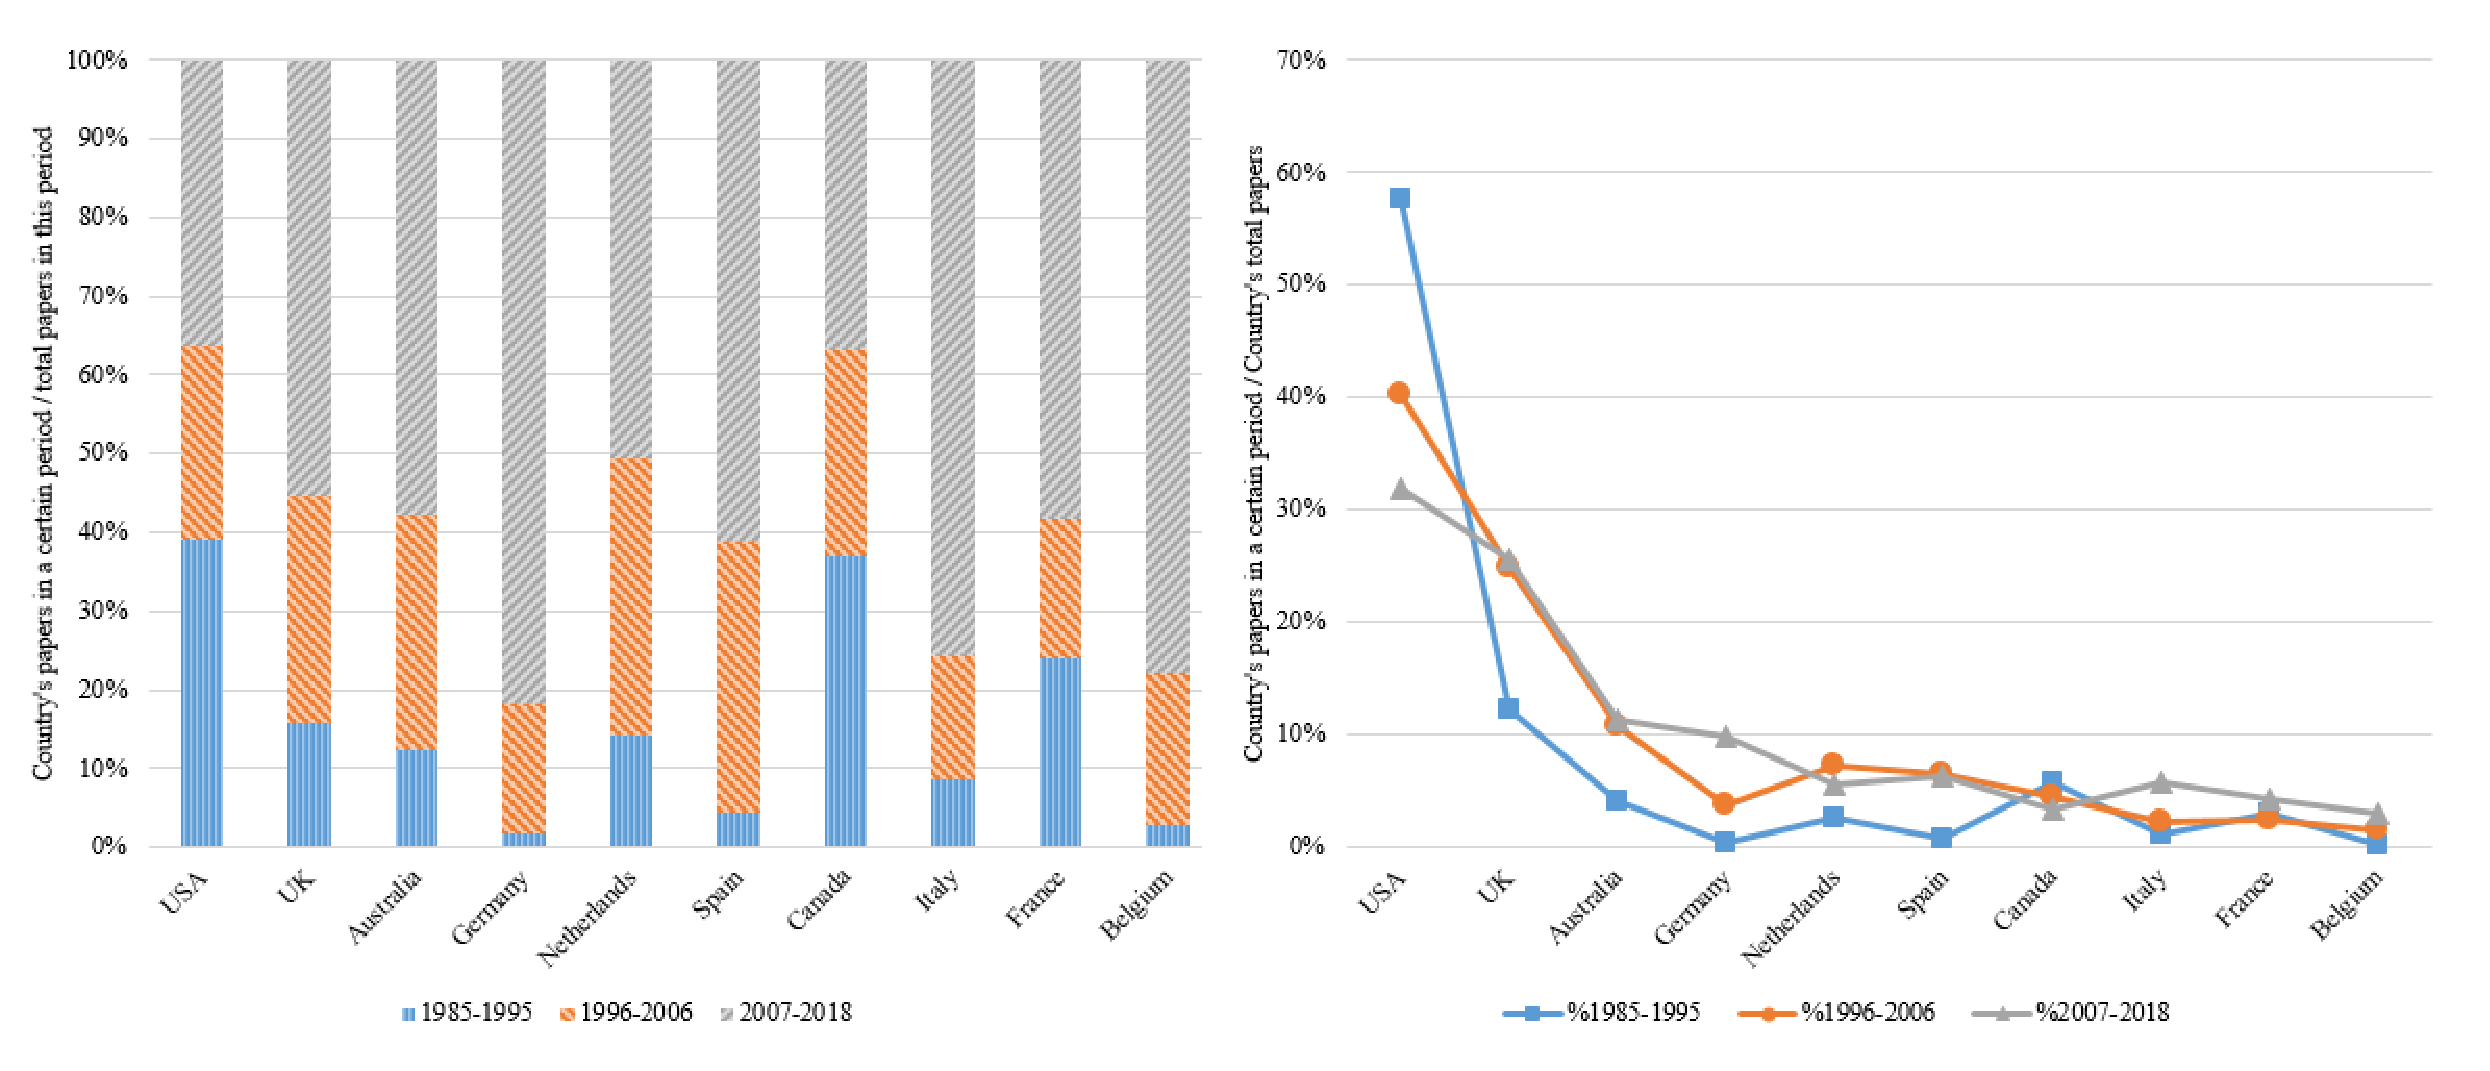
\includegraphics[scale=0.4]{fig.6.eps}
\caption{The dynamic of the academic productivity of the prolific countries}
\end{figure}

The number of citations a country possesses is an important indicator to
evaluate the prestige of it, and also is a sign of knowledge spreading
from the country. Therefore, the top ten most cited countries are
selected in table 7. USA is the most highly cited country, and its
citations are nearly double of the UK' citations. Compared to the table
6, Belgium drops out of the list of top ten most cited countries, and
Turkey replaces Belgium as the member of top most cited countries.
Except for the number of citations, the number of citations per paper is
provided, and it reveals the attraction of single paper. One thing is
interesting that USA dominates the advantage in the total number of
citations, but it is behind Australia, France, Turkey and UK in the
number of citations per paper. What is more, we calculate the number of
citations from the IJF (In-TC) and the number of citations outside the
IJF (Out-TC). The former demonstrates how many IJF researches pay
attention to the papers of the country, and the latter shows the
prestige that the papers of the country possesses outside the IJF. USA
is the most prolific country, but its citation percentage from the IJF
is the lowest, which means its researches caught more attention from
journals outside the IJF. On the contrary, Italy, France, and Germany
possess a relatively high citation percentage from the IJF, which means
these countries receive more endorsements from the researches in IJF
compared with the remaining countries.

\begin{table}
\centering
\caption{The information about the top ten most cited countries}
\setlength{\tabcolsep}{4mm}{
\begin{tabular}{ccccccccc}
\hline
Rank & Country & TC & TP & TC/TP & In-TC & In\% & Out-TC & Out\%\\
\hline
1 & USA & 22875 & 798 & 28.67 & 901 & 3.94\% & 21974 & 96.06\%\\
2 & UK & 12899 & 420 & 30.71 & 646 & 5.01\% & 12253 & 94.99\%\\
3 & Australia & 6540 & 178 & 36.74 & 352 & 5.38\% & 6188 & 94.62\%\\
4 & Netherlands & 2635 & 99 & 26.62 & 150 & 5.69\% & 2485 & 94.31\%\\
5 & France & 2417 & 67 & 36.07 & 226 & 9.35\% & 2191 & 90.65\%\\
6 & Germany & 2023 & 110 & 18.39 & 164 & 8.11\% & 1859 & 91.89\%\\
7 & Spain & 1876 & 93 & 20.17 & 128 & 6.82\% & 1748 & 93.18\%\\
8 & Canada & 1850 & 84 & 22.02 & 121 & 6.54\% & 1729 & 93.46\%\\
9 & Italy & 1122 & 70 & 16.03 & 122 & 10.87\% & 1000 & 89.13\%\\
10 & turkey & 1061 & 33 & 32.15 & 57 & 5.37\% & 1004 & 94.63\%\\
\hline
\end{tabular}}
\end{table}

What is more, a country collaboration network is mapped in Fig. 7. The
size of label denotes the number of papers a country produced, and the
links between any connected labels indicates the collaboration
relationships between connected countries. 25 countries that collaborate
with others no less 15 times are extracted to construct the country
collaboration network. The detailed information including Link (the
collaboration times a country possesses), CM (the country that
collaborate most with the target country), Number (the collaboration
times that CM collaborates with the target country) and N/L (the
percentage that divides Number by Link) is stated in table 8. USA ranks
the first in table 8 with 217 collaboration times, followed by UK with
201 collaboration times. Moreover, USA and UK are the countries that
cooperate with each other the most. Besides, 11 countries cooperate with
USA the most, and 9 countries cooperate with UK the most. Australia
ranks the third in table 8, but it is not the most collaborated country
to any of the countries in table 8, while Netherlands is the most
collaborated country to Belgium, Denmark, and Austria.

\begin{figure}[htbp]
\centering
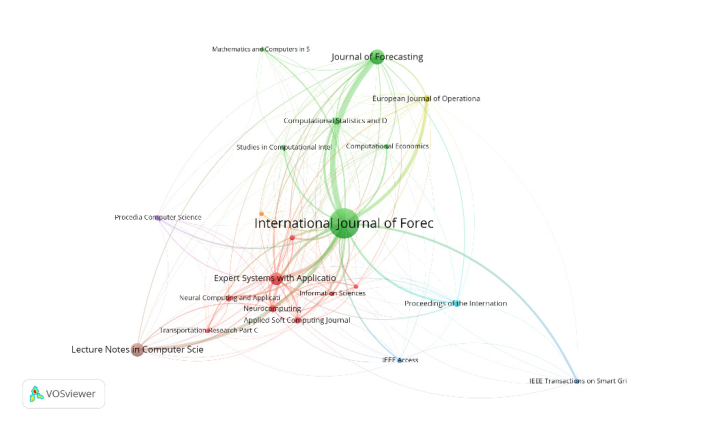
\includegraphics[scale=0.4]{fig.7.eps}
\caption{Country collaboration network}
\end{figure}

\begin{table}
\centering
\caption{Information about the countries in the country collaboration network}
\setlength{\tabcolsep}{7mm}{
\begin{tabular}{cccccc}
\hline
Rank & Country & Link & CM & Number & N/L\\
\hline
1 & USA & 217 & UK & 44 & 20.28\%\\
2 & UK & 201 & USA & 44 & 21.89\%\\
3 & Australia & 116 & US & 42 & 36.21\%\\
4 & Netherlands & 69 & USA/Belgium & 8 & 11.59\%\\
5 & Germany & 61 & USA & 14 & 22.95\%\\
6 & Italy & 57 & UK & 21 & 36.84\%\\
7 & Canada & 54 & USA & 19 & 35.19\%\\
8 & France & 49 & UK & 15 & 30.61\%\\
9 & Spain & 39 & UK & 13 & 33.33\%\\
10 & Belgium & 34 & Netherlands/UK & 8 & 23.53\%\\
11 & Denmark & 32 & Netherlands & 7 & 21.88\%\\
12 & Turkey & 30 & UK & 12 & 40.00\%\\
13 & Switzerland & 20 & USA & 4 & 20.00\%\\
14 & Brazil & 19 & UK & 6 & 31.58\%\\
15 & China & 19 & USA & 9 & 47.37\%\\
16 & Sweden & 15 & Netherlands & 4 & 26.67\%\\
17 & Taiwan & 14 & USA & 5 & 35.71\%\\
18 & Norway & 12 & Italy & 4 & 33.33\%\\
19 & Greece & 11 & UK & 6 & 54.55\%\\
20 & New Zealand & 11 & USA & 6 & 54.55\%\\
21 & South Korea & 11 & USA & 8 & 72.73\%\\
22 & Austria & 10 & Germany & 5 & 50.00\%\\
23 & Japan & 10 & USA/Japan & 3 & 30.00\%\\
24 & Portugal & 8 & Spain/USA & 3 & 37.50\%\\
25 & Finland & 7 & Sweden/UK/USA & 2 & 28.57\%\\
\hline
\end{tabular}}
\end{table}

\section{Knowledge diffusion analysis of the forecasting
journals}\label{knowledge-diffusion-analysis-of-the-forecasting-journals}

In academics, knowledge diffuses along with the citing behaviors of
papers, and papers belong to different subject areas according to their
research contents. In Scopus, subject areas are usually considered as
the labels to classify the different kinds of knowledge. In this study,
subject areas are used for conducting the knowledge diffusion analysis.
However, categorizations on subject areas exist deviations because of
the informal acquisition (Leydesdorff and Goldstone 2014), therefore,
the analysis only relying on the level of subject areas is easily to be
subject to a biased result. For this reason, the knowledge diffusion
analysis is conducted both at the subject area level and the journal
level.

As one of the leading forecasting journal, IJF was launched in 1985
following another authoritative forecasting journal, Journal of
Forecasting (JF). These two leading forecasting journals are the
important members in the International Institute of Forecasting (IIF).
Therefore, in this study, in order to have a broader overview about the
knowledge fertilization in the forecasting field, both of IJF and JF are
included in the knowledge diffusion analysis.

\subsection{Analysis at the level of subject
area}\label{analysis-at-the-level-of-subject-area}

In this subsection, papers cited IJF and JF papers are selected,
respectively, as the raw data. A static analysis about the subject area
distribution is provided to figure out which subject areas pay attention
to the forecasting papers. Moreover, a dynamic analysis is supplemented
to describe how the subject area distribution evolves over time.
Forecasting papers in different periods may attract researches from
different subject areas.

\subsubsection{Static analysis about the subject area
distribution}\label{static-analysis-about-the-subject-area-distribution}

In Scopus, IJF papers ranging from 1985 to 2018 was retrieved, and then
29464 citing papers ranging from 1985 to 2019 were harvested. Similarly,
16419 citing papers are obtained based on JF papers from 1982 to 2018.
The top ten most prolific subject areas among the citing papers are
stated in table 9. We find that IJF citing papers and JF citing papers
possess the same prolific subject areas, which denotes both of the
journals have very similar audiences. IJF and JF were set with an aim
that become an output for the BEM forecasting researches (Fildes 2006).
From the angle of knowledge diffusion, this aim has been successfully
achieved because Computer Science, Economics, Econometrics and Finance,
and Business, Management and Accounting have become the three dominant
subject areas based on the forecasting citing papers.

\begin{table}[!htbp]
    \centering
    \caption{Information about the top ten most prolific subject areas}
    \setlength{\tabcolsep}{1mm}{
    \begin{tabular}{c c c c|c c c c}
        \hline
        \multicolumn{4}{c|}{29464 citing papers of IJF} & \multicolumn{4}{c}{16419 citing papers of JF}\\
        \hline
        Rank & Subject area & NP1 & Percent1 & Rank & Subject area & NP2 & Percent2\\
        \hline
        1 & Computer Science & 7586 & 25.75\% & 1 & \makecell[c]{Economics, Econometrics \\ and Finance} & 5184 & 31.57\%\\
        2 & \makecell[c]{Economics, Econometrics \\ and Finance} & 7487 & 25.41\% & 2 & \makecell[c]{Business, Management \\ and Accounting} & 4891 & 29.79\%\\
    3 & \makecell[c]{Business, Management \\ and Accounting} & 7449 & 25.28\% & 3 & Mathematics & 3946 & 24.03\%\\
    4 & Engineering & 5888 & 19.98\% & 4 & Computer Science & 3791 & 23.09\%\\
    5 & Mathematics & 5482 & 18.61\% & 5 & Decision Sciences & 2971 & 18.09\%\\
    6 & Social Sciences & 4277 & 14.52\% & 6 & Engineering & 2305 & 14.04\%\\
    7 & Decision Sciences & 3665 & 12.44\% & 7 & Social Sciences & 2179 & 13.27\%\\
    8 & Energy & 2222 & 7.54\% & 8 & Environmental Science & 1109 & 6.75\%\\
    9 & Environmental Science & 2070 & 7.03\% & 9 & Energy & 641 & 3.90\%\\
    10 & Earth and Planetary Sciences & 969 & 3.29\% & 10 & Earth and Planetary Sciences & 588 & 3.58\%\\
        \hline
    \end{tabular}}
\end{table}

\subsubsection{Dynamic analysis about the subject area
distribution}\label{dynamic-analysis-about-the-subject-area-distribution}

To better explore the dynamic of the subject area distribution, the IJF
citing papers are divided into three slices based on their publishing
years. In each period, the top ten prolific subject areas are provided,
as shown in table 10. Computer Science and Engineering are two subject
areas that keep moving up over three periods, which means the IJF papers
attract increasingly researches on both of these subject areas. More and
more forecasting papers pay attention to the combination with researches
on these two subject areas, and these two subject areas would possibly
continue to be the research hotspot in the next few years. The ranking
of Psychology keeps declining over three periods from the seventh in
1985-1996 to the tenth in 1997-2008, finally falling out of the list in
2009-2019. Also there has been a marked pullback in the ranking of
Decision Sciences from period 1 to period 2.

Similar work is conducted in the JF citing papers, and the top ten
prolific subject areas are provided in table 11. \emph{Economics,
Econometrics and Finance}, \emph{Computer Science}, and
\emph{Engineering} are three subject areas that keep moving up during
three periods, while the rankings of \emph{Decision Sciences}, and
\emph{Psychology} decline over time. It indicates that the former three
subject areas are the research hotspots in the current forecasting
field, and the latter two are in a declining position.

\newpage

\begin{table}[!htbp]
    \centering
    \caption{Change of subject area distribution in IJF citing papers over time}
    \setlength{\tabcolsep}{1mm}{
    \begin{tabular}{c c c|c c c|c c c}
        \hline
        \hline
        \multicolumn{3}{c|}{1985-1996} & \multicolumn{3}{c|}{1997-2008} & \multicolumn{3}{c}{1997-2008}\\
    \hline
    \multicolumn{3}{c|}{1046 IJF citing papers} & \multicolumn{3}{c|}{5312 IJF citing papers} & \multicolumn{3}{c}{23105 IJF citing papers}\\
    \hline
    Subject area & NP1 & Percent1 & Subject area & NP2 & Percent2 & Subject area & NP3 & Percent3\\
        \hline
        \hline
        \makecell[c]{Business,\\ Management \\ and Accounting} & 586 & 56.02\% & \makecell[c]{Business,\\ Management \\ and Accounting} & 1708 & 32.15\% & Computer Science & 6259 & 27.09\%\\
        \hline
        \makecell[c]{Economics,\\ Econometrics \\ and Finance} & 269 & 25.72\% &      \makecell[c]{Economics,\\ Econometrics \\ and Finance} & 1485 & 27.96\% & \makecell[c]{Economics,\\ Econometrics \\ and Finance} & 5733 & 24.81\%\\
        \hline
    Decision Sciences & 246 & 23.52\% & Computer Science & 1185 & 22.31\% & \makecell[c]{Business,\\ Management \\ and Accounting} & 5155 & 22.31\%\\
    \hline
    Mathematics & 226 & 21.61\% & Mathematics & 1034 & 19.47\% & Engineering & 4944 & 21.40\%\\
    \hline
    Social Sciences & 157 & 15.01\% & Engineering & 878 & 16.53\% & Mathematics & 4222 & 18.27\%\\
    \hline
    Computer Science & 141 & 13.48\% & Social Sciences & 869 & 16.36\% & Social Sciences & 3251 & 14.07\%\\
    \hline
    Engineering & 65 & 6.21\% & Decision Sciences & 835 & 15.72\% & Decision Sciences & 2584 & 11.18\%\\
    \hline
    Psychology & 65 & 6.21\% & \makecell[c]{Environmental\\ Science} & 311 & 5.85\% & energy & 2068 & 8.95\%\\
    \hline
    \makecell[c]{Environmental\\ Science} & 44 & 4.21\% & \makecell[c]{Earth and\\ Planetary\\ Sciences} & 190 & 3.58\% & \makecell[c]{Environmental\\ Science} & 1715 & 7.42\%\\
    \hline
    Arts and Humanities & 22 & 2.10\% & Psychology & 173 & 3.26\% & \makecell[c]{Earth and\\ Planetary\\ Sciences} & 765 & 3.31\%\\
        \hline
        \hline
    \end{tabular}}
\end{table}\begin{table}[H]
    \centering
    \caption{Change of subject area distribution in JF citing papers over time}
    \setlength{\tabcolsep}{1.1mm}{
    \begin{tabular}{c c c|c c c|c c c}
        \hline
        \hline
        \multicolumn{3}{c|}{1982-1994} & \multicolumn{3}{c|}{1995-2007} & \multicolumn{3}{c}{2008-2019}\\
    \hline
    \multicolumn{3}{c|}{1272 JF citing papers} & \multicolumn{3}{c|}{4117 JF citing papers} & \multicolumn{3}{c}{11209 JF citing papers}\\
    \hline
    Subject area & NP1 & Percent1 & Subject area & NP2 & Percent2 & Subject area & NP3 & Percent3\\
        \hline
        \hline
        \makecell[c]{Business,\\ Management \\ and Accounting} & 696 & 54.72\% & \makecell[c]{Business,\\ Management \\ and Accounting} & 1290 & 31.33\% & \makecell[c]{Economics,\\ Econometrics \\ and Finance} & 3756 & 34.06\%\\
        \hline
Decision Sciences & 437 & 34.36\% & \makecell[c]{Economics,\\ Econometrics \\ and Finance} & 1177 & 28.59\% & \makecell[c]{Business,\\ Management \\ and Accounting} & 2905 & 26.34\%\\
    \hline
Mathematics & 388 & 30.50\% & Mathematics & 1114 & 27.06\% & Computer Science & 2651 & 24.04\%\\
    \hline
Computer Science & 262 & 20.60\% & Computer Science & 878 & 21.33\% & Mathematics & 2444 & 22.16\%\\
    \hline
\makecell[c]{Economics,\\ Econometrics \\ and Finance} & 250 & 19.65\% & Decision Sciences & 866 & 21.03\% & Engineering & 17537 & 159.01\%\\
    \hline
Social Sciences & 198 & 15.57\% & Social Sciences & 559 & 13.58\% & Decision Sciences & 1668 & 15.12\%\\
    \hline
Psychology & 134 & 10.53\% & Engineering & 472 & 11.46\% & Social Sciences & 1422 & 12.89\%\\
    \hline
Engineering & 80 & 6.29\% & \makecell[c]{Environmental\\Science} & 313 & 7.60\% & \makecell[c]{Environmental\\Science} & 734 & 6.66\%\\
    \hline
\makecell[c]{Environmental\\Science} & 62 & 4.87\% & \makecell[c]{Earth and\\Planetary\\Sciences} & 208 & 5.05\% & Energy & 563 & 5.10\%\\
    \hline
\makecell[c]{Arts and\\Humanities} & 61 & 4.80\% & Psychology & 183 & 4.44\% & \makecell[c]{Earth and\\ Planetary\\Sciences} & 348 & 3.16\%\\
    \hline
        \hline
    \end{tabular}}
\end{table}

\subsection{Analysis at the level of
journal}\label{analysis-at-the-level-of-journal}

Based on the subsection 3.1, the knowledge diffusion analysis at the
level of subject area has been completed, but the scope of subject area
is kind of wide-ranging. Therefore, the research scope is narrowed to
the level of journal to conduct a further knowledge diffusion analysis.
The subject areas which have a special performance in subsection 3.1
will be analyzed as the primary research objectives, and the citation
relationships between different journals within the same subject area
will be elaborated and visualized in citation networks. Moreover, all of
the analysis is dynamic to better elaborate the evolution progress of
the knowledge diffusion among the different journals. Considering the
authority of IJF and JF in the forecasting field, the knowledge
diffusion processes starting from IJF and JF are both delineated based
on their citations relationships. The forecasting-related applications
published in the journals outside the forecasting journals are
investigated.

\subsubsection{Knowledge diffusion within the same subject area starts
from
IJF}\label{knowledge-diffusion-within-the-same-subject-area-starts-from-ijf}

Knowledge diffusion starts from IJF has been investigated in subsection
3.1.2, and four subject areas have a special performance, which are
Computer Science, Engineering, Psychology, and Decision Sciences. All of
the citing papers belonging to these four subject areas are harvested,
respectively, then aggregated into the level of journal, and the journal
citation relationships between different journals within the same
subject area are extracted and mapped in journal citation networks.

\noindent 3.2.1.1. Journal citation network in Computer Science

All the citing papers belonging to Computer Science are harvested and
divided into three periods. In each period, the journal citation
relationships are mapped in Fig. 8-10, and the journal citation
structure can be intuitively observed in Fig. 8-10. Given the different
scale of journal networks, there are different limiting conditions set
for three networks, and then different parameters of each network
including clusters (the number of groups containing the same color
nodes), local links (the number of links), and link strength (the total
strength that each link possesses). The top ten journals that have the
most connections with IJF are extracted. Note that the information about
the limiting conditions, parameters, and top ten journals is stated in
table 12.

\begin{figure}[!htbp]
\centering
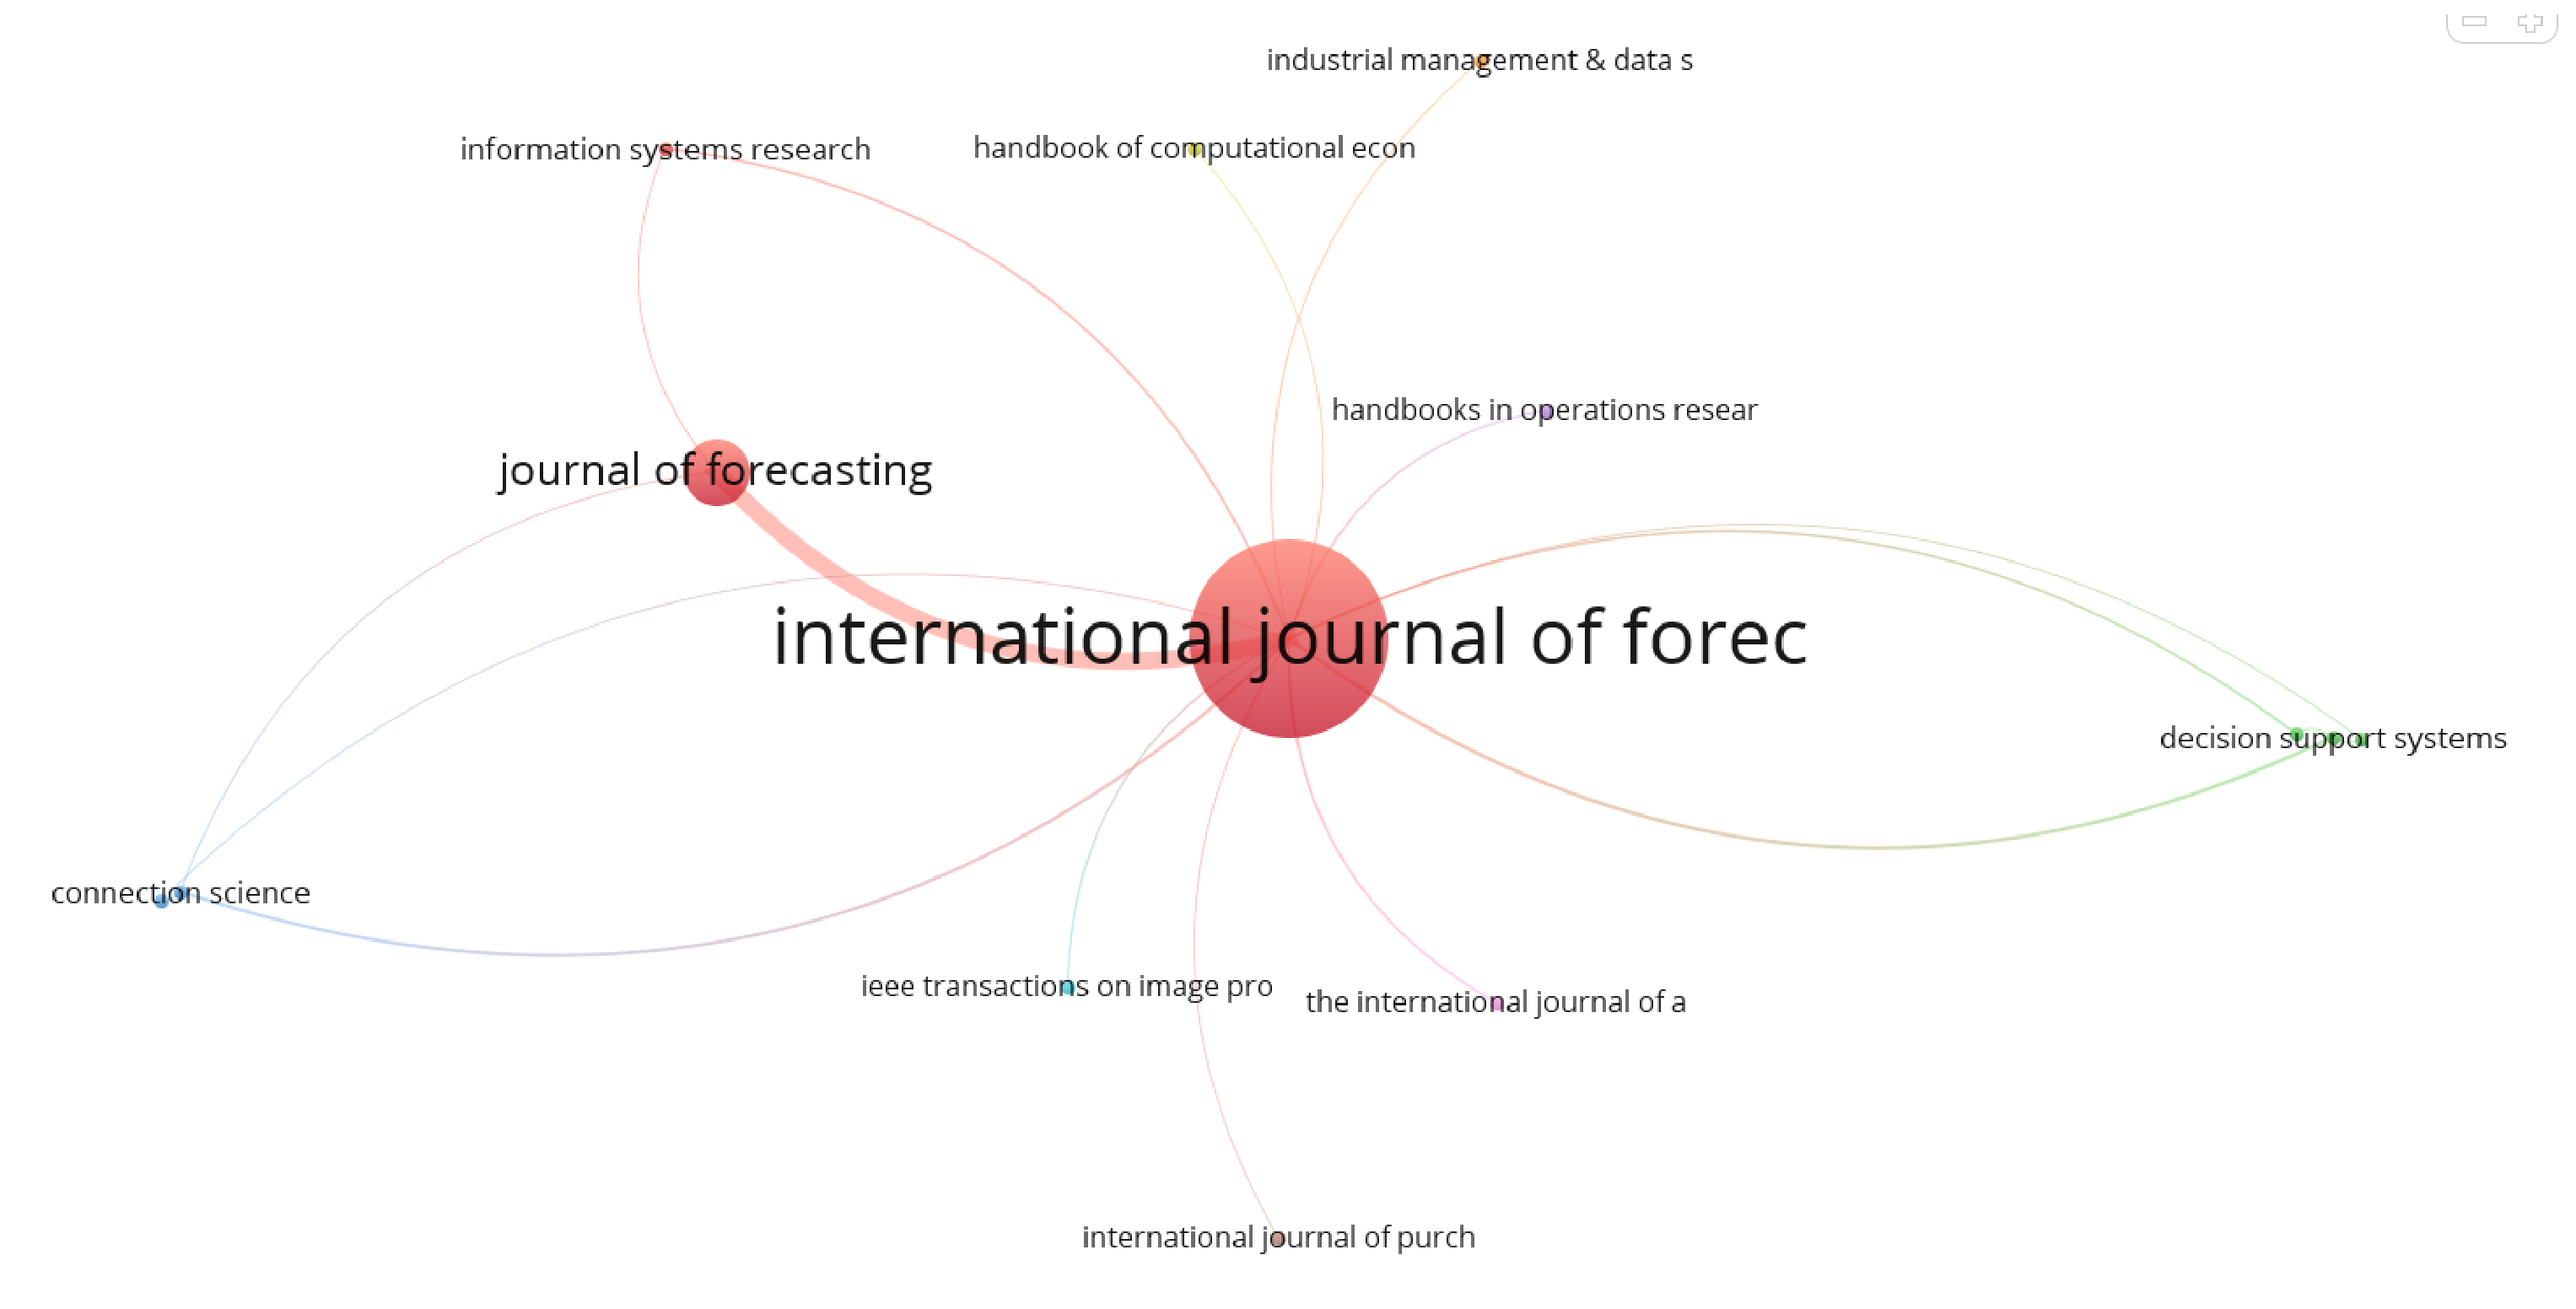
\includegraphics[scale=0.3]{fig.8.eps}
\caption{ IJF Journal citation network in Computer Science from 1985 to 1994}
\end{figure}

\begin{figure}[!htbp]
\centering
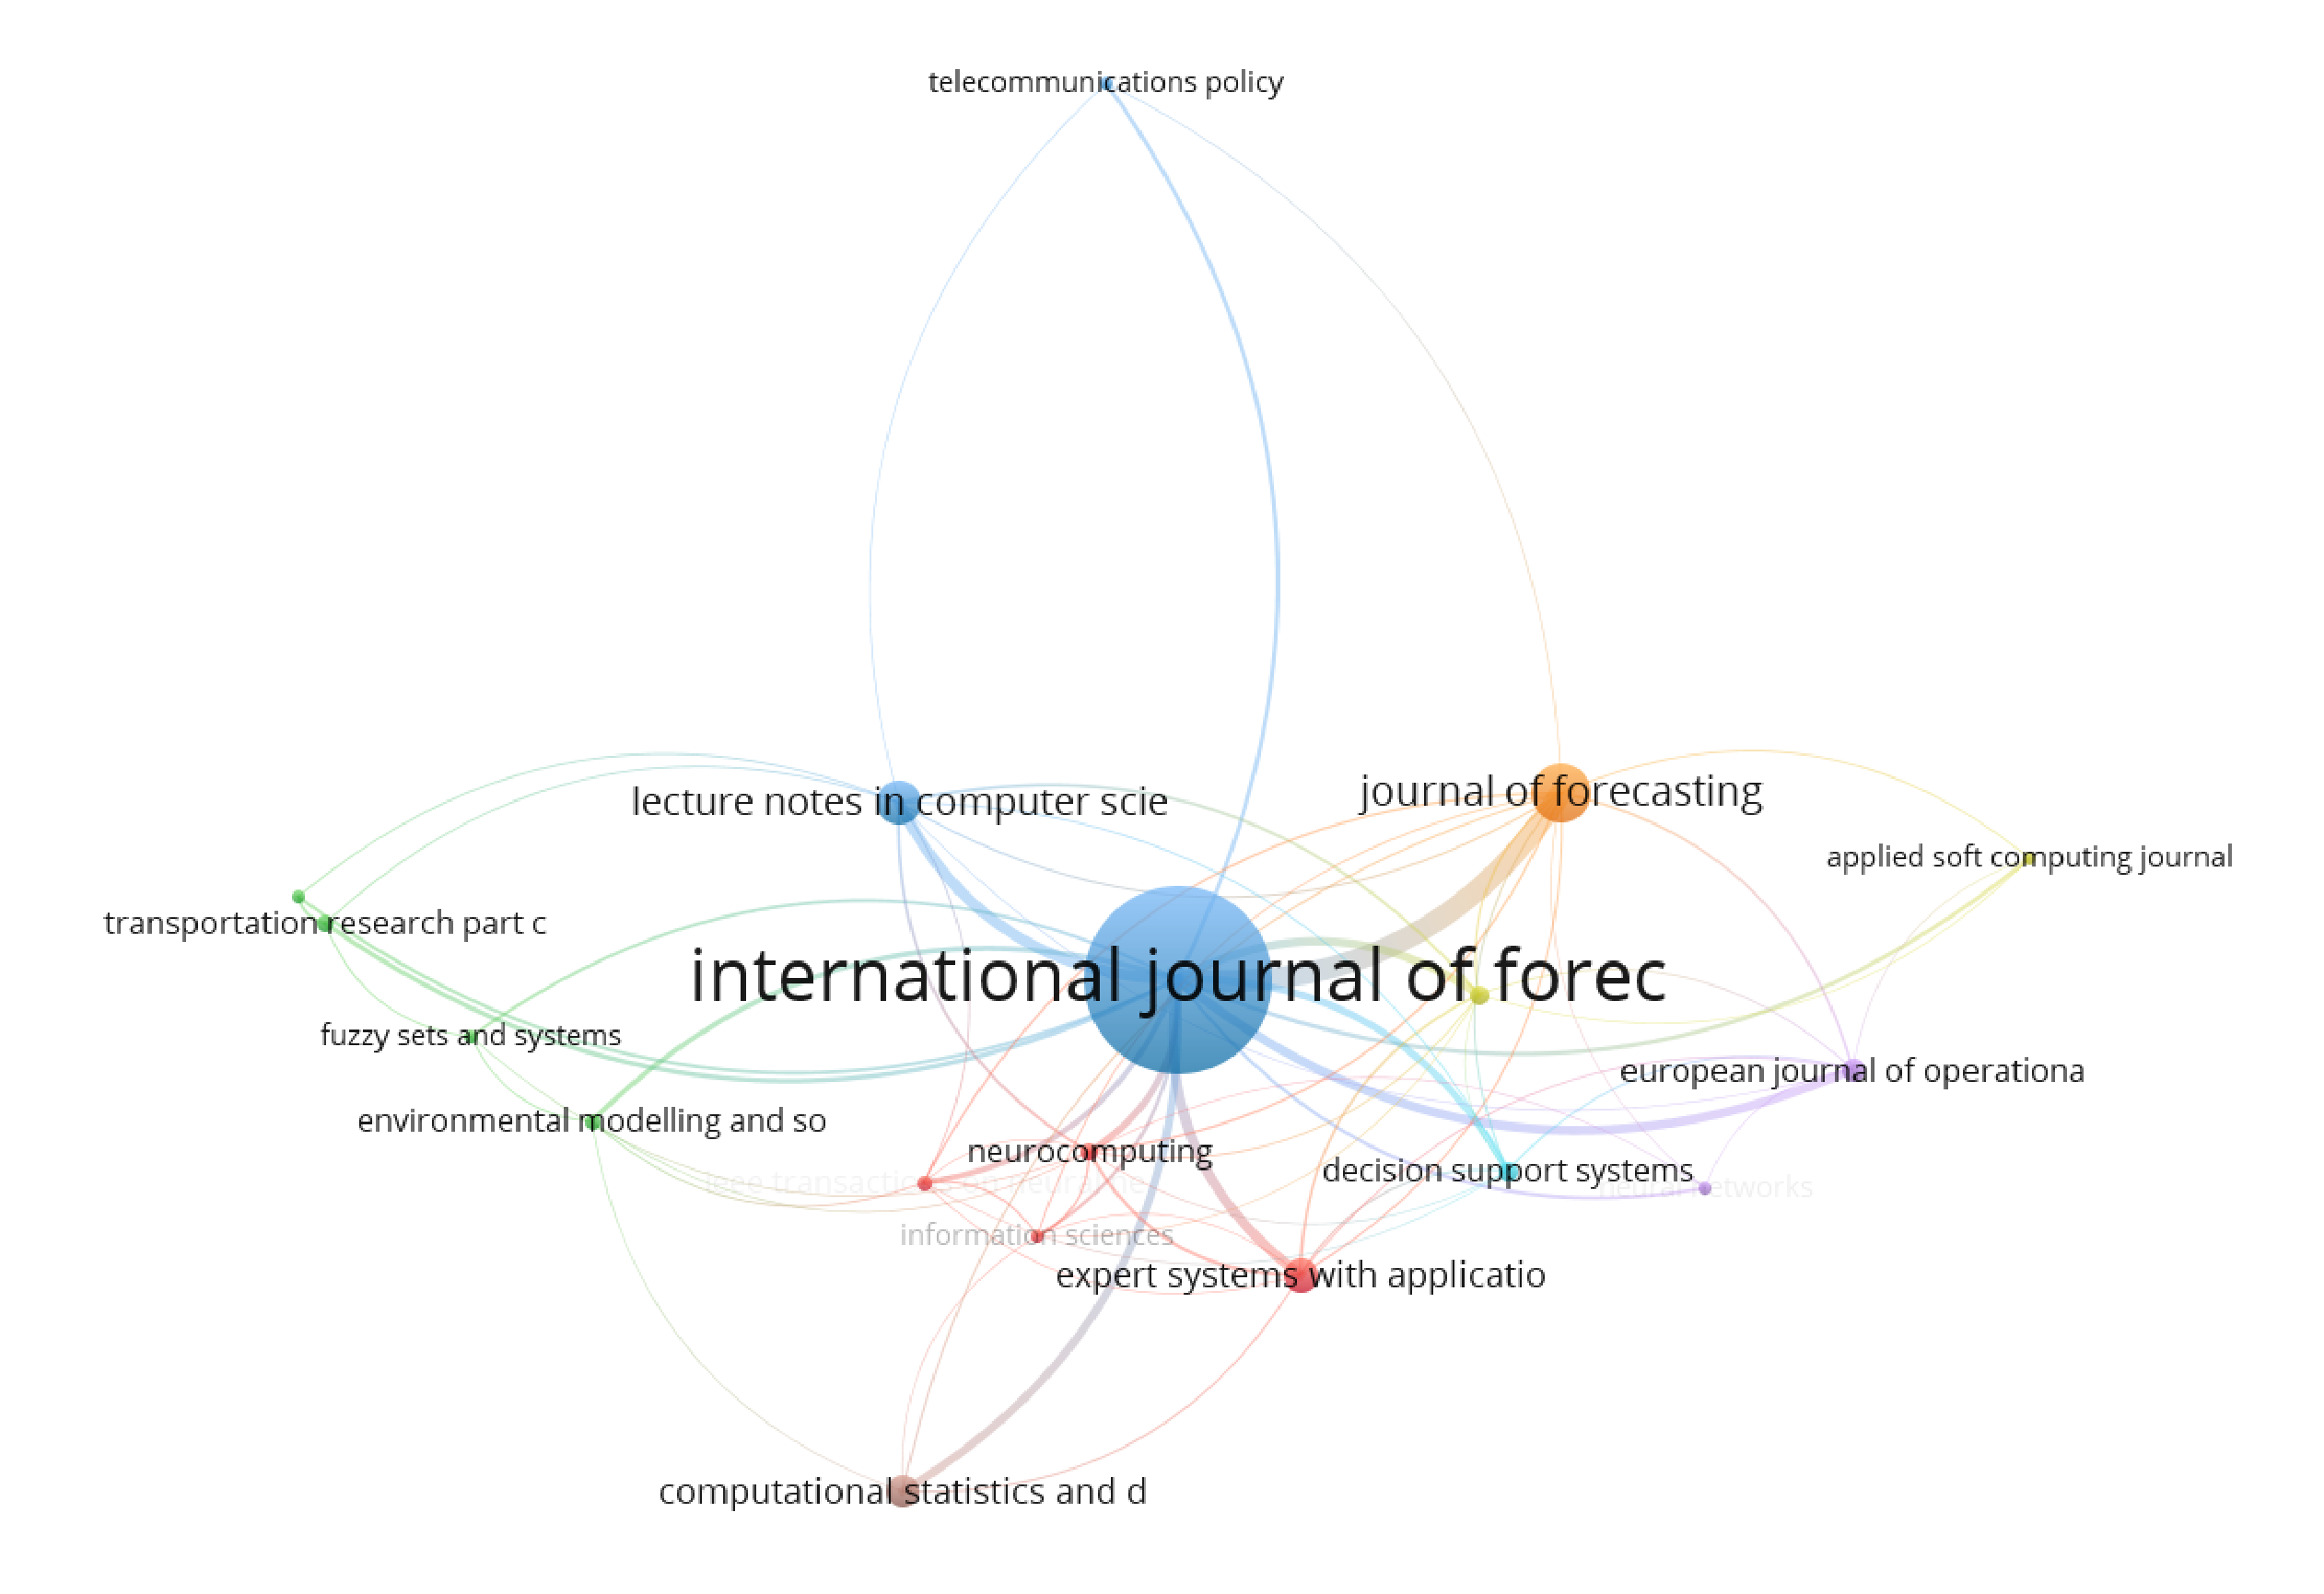
\includegraphics[scale=0.3]{fig.9.eps}
\caption{ IJF Journal citation network in Computer Science from 1997 to 2008}
\end{figure}

\begin{figure}[!htbp]
\centering
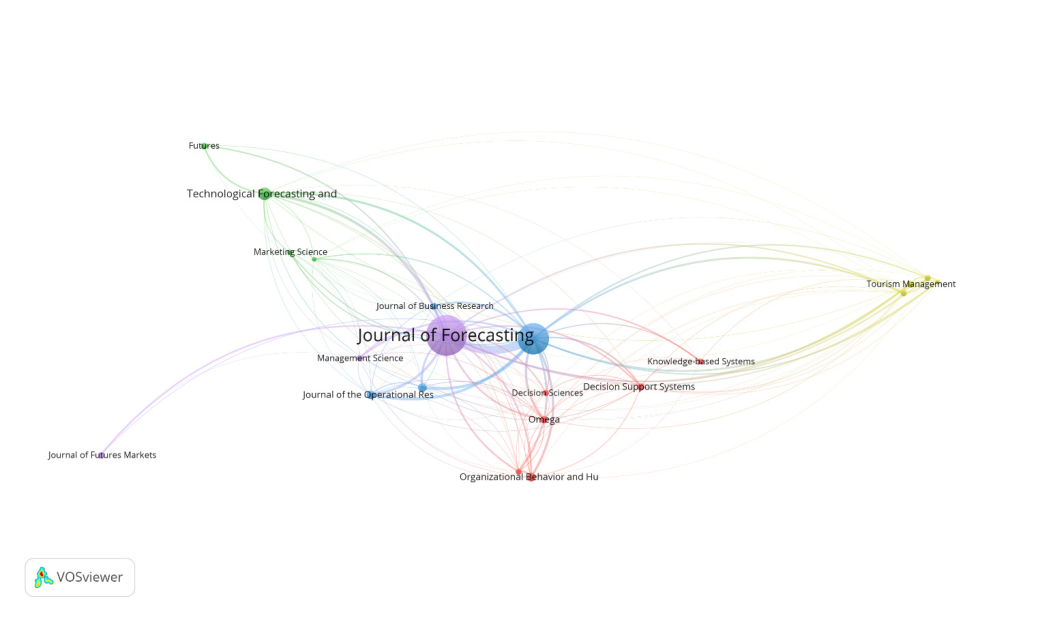
\includegraphics[scale=0.3]{fig.10.eps}
\caption{ IJF Journal citation network in Computer Science from 2009 to 2019}
\end{figure}

\begin{landscape}
\begin{table}[!htbp]
    \centering
    \caption{The information about the journal citation networks in Computer Science based on the IJF citing papers}
    \setlength{\tabcolsep}{0.3mm}{
    \begin{tabular}{p{1.5cm}<{\centering} p{6cm}<{\centering} p{1.5cm}<{\centering}|p{1.5cm}<{\centering} p{6cm}<{\centering} p{1.5cm}<{\centering}|p{1.5cm}<{\centering} p{6cm}<{\centering} p{1.5cm}<{\centering}}
    \hline
        \hline
        \multicolumn{3}{c|}{1985-1996} & \multicolumn{3}{c|}{1997-2008} & \multicolumn{3}{c}{2009-2019}\\
    \hline
    \multicolumn{9}{c}{Limiting condition}\\
    \hline
        \multicolumn{3}{c|}{Number>=1 Citation>=10} & \multicolumn{3}{c|}{Number>=5 Citation>=200} & \multicolumn{3}{c}{Number>=40 Citation>=200}\\
    \hline
    \multicolumn{9}{c}{Parameters}\\
    \hline
    Clusters & Local links & Link strength & Clusters & Local links & Link strength & Clusters & Local links & Link strength\\
    9 & 18 & 173 & 8    & 66 & 1025 & 7 & 168 & 6146\\
        \hline
        \hline
    R & Journal & Links & R & Journal & Links & R & Journal & Links\\
   1 & Journal of Forecasting & 139 & 1 & Journal of Forecasting & 365 & 1 & Journal of Forecasting & 1448\\
   2 & Decision Support Systems & 6 & 2 & Lecture Notes in Computer Science & 93 & 2 & Expert Systems with Applications & 550\\
   3 & Connection Science & 5 & 3 & Expert Systems with Applications & 76 & 3 & Lecture Notes in Computer Science & 429\\
   4 & Expert Systems & 3 & 4 & European Journal of Operational Research & 62 & 4 & European Journal of Operational Research & 300\\
   5 & Information Systems Research & 3 & 5 & Computers and Operations Research & 54 & 5 & Neurocomputing & 249\\
   6 & \makecell[c]{The International Journal of Advanced\\Manufacturing Technology} & 3 & 6 & Computational Statistics and Data Analysis & 53 & 6 & Computational Statistics and Data Analysis & 214\\
   7 & \makecell[c]{Handbooks in Operations Research and\\Management Science} & 2 & 7 & Decision Support Systems & 39 & 7 & Proceedings of The International Joint Conference on Neural Networks & 173\\
   8 & IEEE Transactions on Image Processing & 2 & 8 & Neurocomputing & 36 & 8 & Applied Soft Computing Journal & 156\\
   9 & IEEE Transactions on Neural Networks & 1 & 9 & IEEE Transactions on Neural Networks & 24 & 9 & Decision Support Systems & 149\\
   10 & The Knowledge Engineering Review & 1 & 10 & Environmental Modelling and Software & 20 & 10 & IEEE Transactions on Smart Grid & 134\\
  \hline
  \hline
    \end{tabular}}
\end{table}
\end{landscape}

Observing from the Fig. 8-10, IJF always occupies a central place in
networks with other connected journals around it. JF is the journal that
possesses the most connection with IJF, which indicates IJF is most
cited by the papers of JF. The structure of the three networks has some
little change from period 1 to period 3. Except for JF, Lecture Notes in
Computer Science, and Expert Systems with Applications and European
Journal of Operational Research are three journals that gradually
possess increasingly thicker links with IJF, which means they take an
increasingly important position in their journal citation networks.
Information in the table 12 also proves the fact that these three
journals have the most citation connection with IJF comparing with other
journals, and they are the most royal audiences of IJF. Moreover, except
for JF and Decision Support Systems, all of the top journals in period 1
fall out of the lists in period 2 and 3. The ranking of Decision Support
Systems keeps declining over time. This phenomenon denotes that there is
a big change in the audience of IJF from period 1 to period 2 and 3, and
it is an interesting finding that is worthy of a deeper investigation in
the future work.

\noindent 3.2.1.2. Journal citation network in Engineering

The journal citation relationships based on the citing papers belonging
to Engineering are depicted in the Fig. 11-13, and the detailed
information is stated in table 13. From the structure of networks, IJF
is a dominating center, and the links connecting IJF and other journals
are increasingly thicker over time. From period 1 to 3, International
Journal of Production Research (IJPR) is the only one journal that
appears in three networks, but its ranking keeps declining over time,
which means IJPR is a relatively royal audience of IJF but IJF is
becoming more attractive to other journals than to IJPR over time.
Moreover, except for IJPR, all of the journals in the list of period 1
disappear in the lists of period 2 and 3, which means there exists a big
change in the top journals of Engineering from period 1 to period 2 and
3. Expert Systems with Applications, International Journal of Production
Economics, and IEEE Transactions on Power Systems are journals that have
a good performance both in period 2 and 3, which means they are
interested in the IJF papers and become the main citing journals of IJF
for a relatively long time. One thing is interesting that unlike the
leading position occupies in Computer Science, JF only appears in the
list of period 2 in table 13, which demonstrates JF performs less well
in Engineering than in Computer Science. The citation connection between
IJF and JF in Engineering is much weaker than in Computer Science.
Besides, observing from Fig. 13, there is an emerging cluster containing
some red nodes in the left side of the figure, which has not appeared in
both Fig. 11 and 12. According to the table 13, they are some
energy-related journals which are Energy, Energies, Applied Energy, and
International Journal of Electrical Power and Energy Systems. It is an
important signal that some energy-related journals in Engineering are
becoming more and more interested in the IJF researches.

\begin{figure}[htbp]
\centering
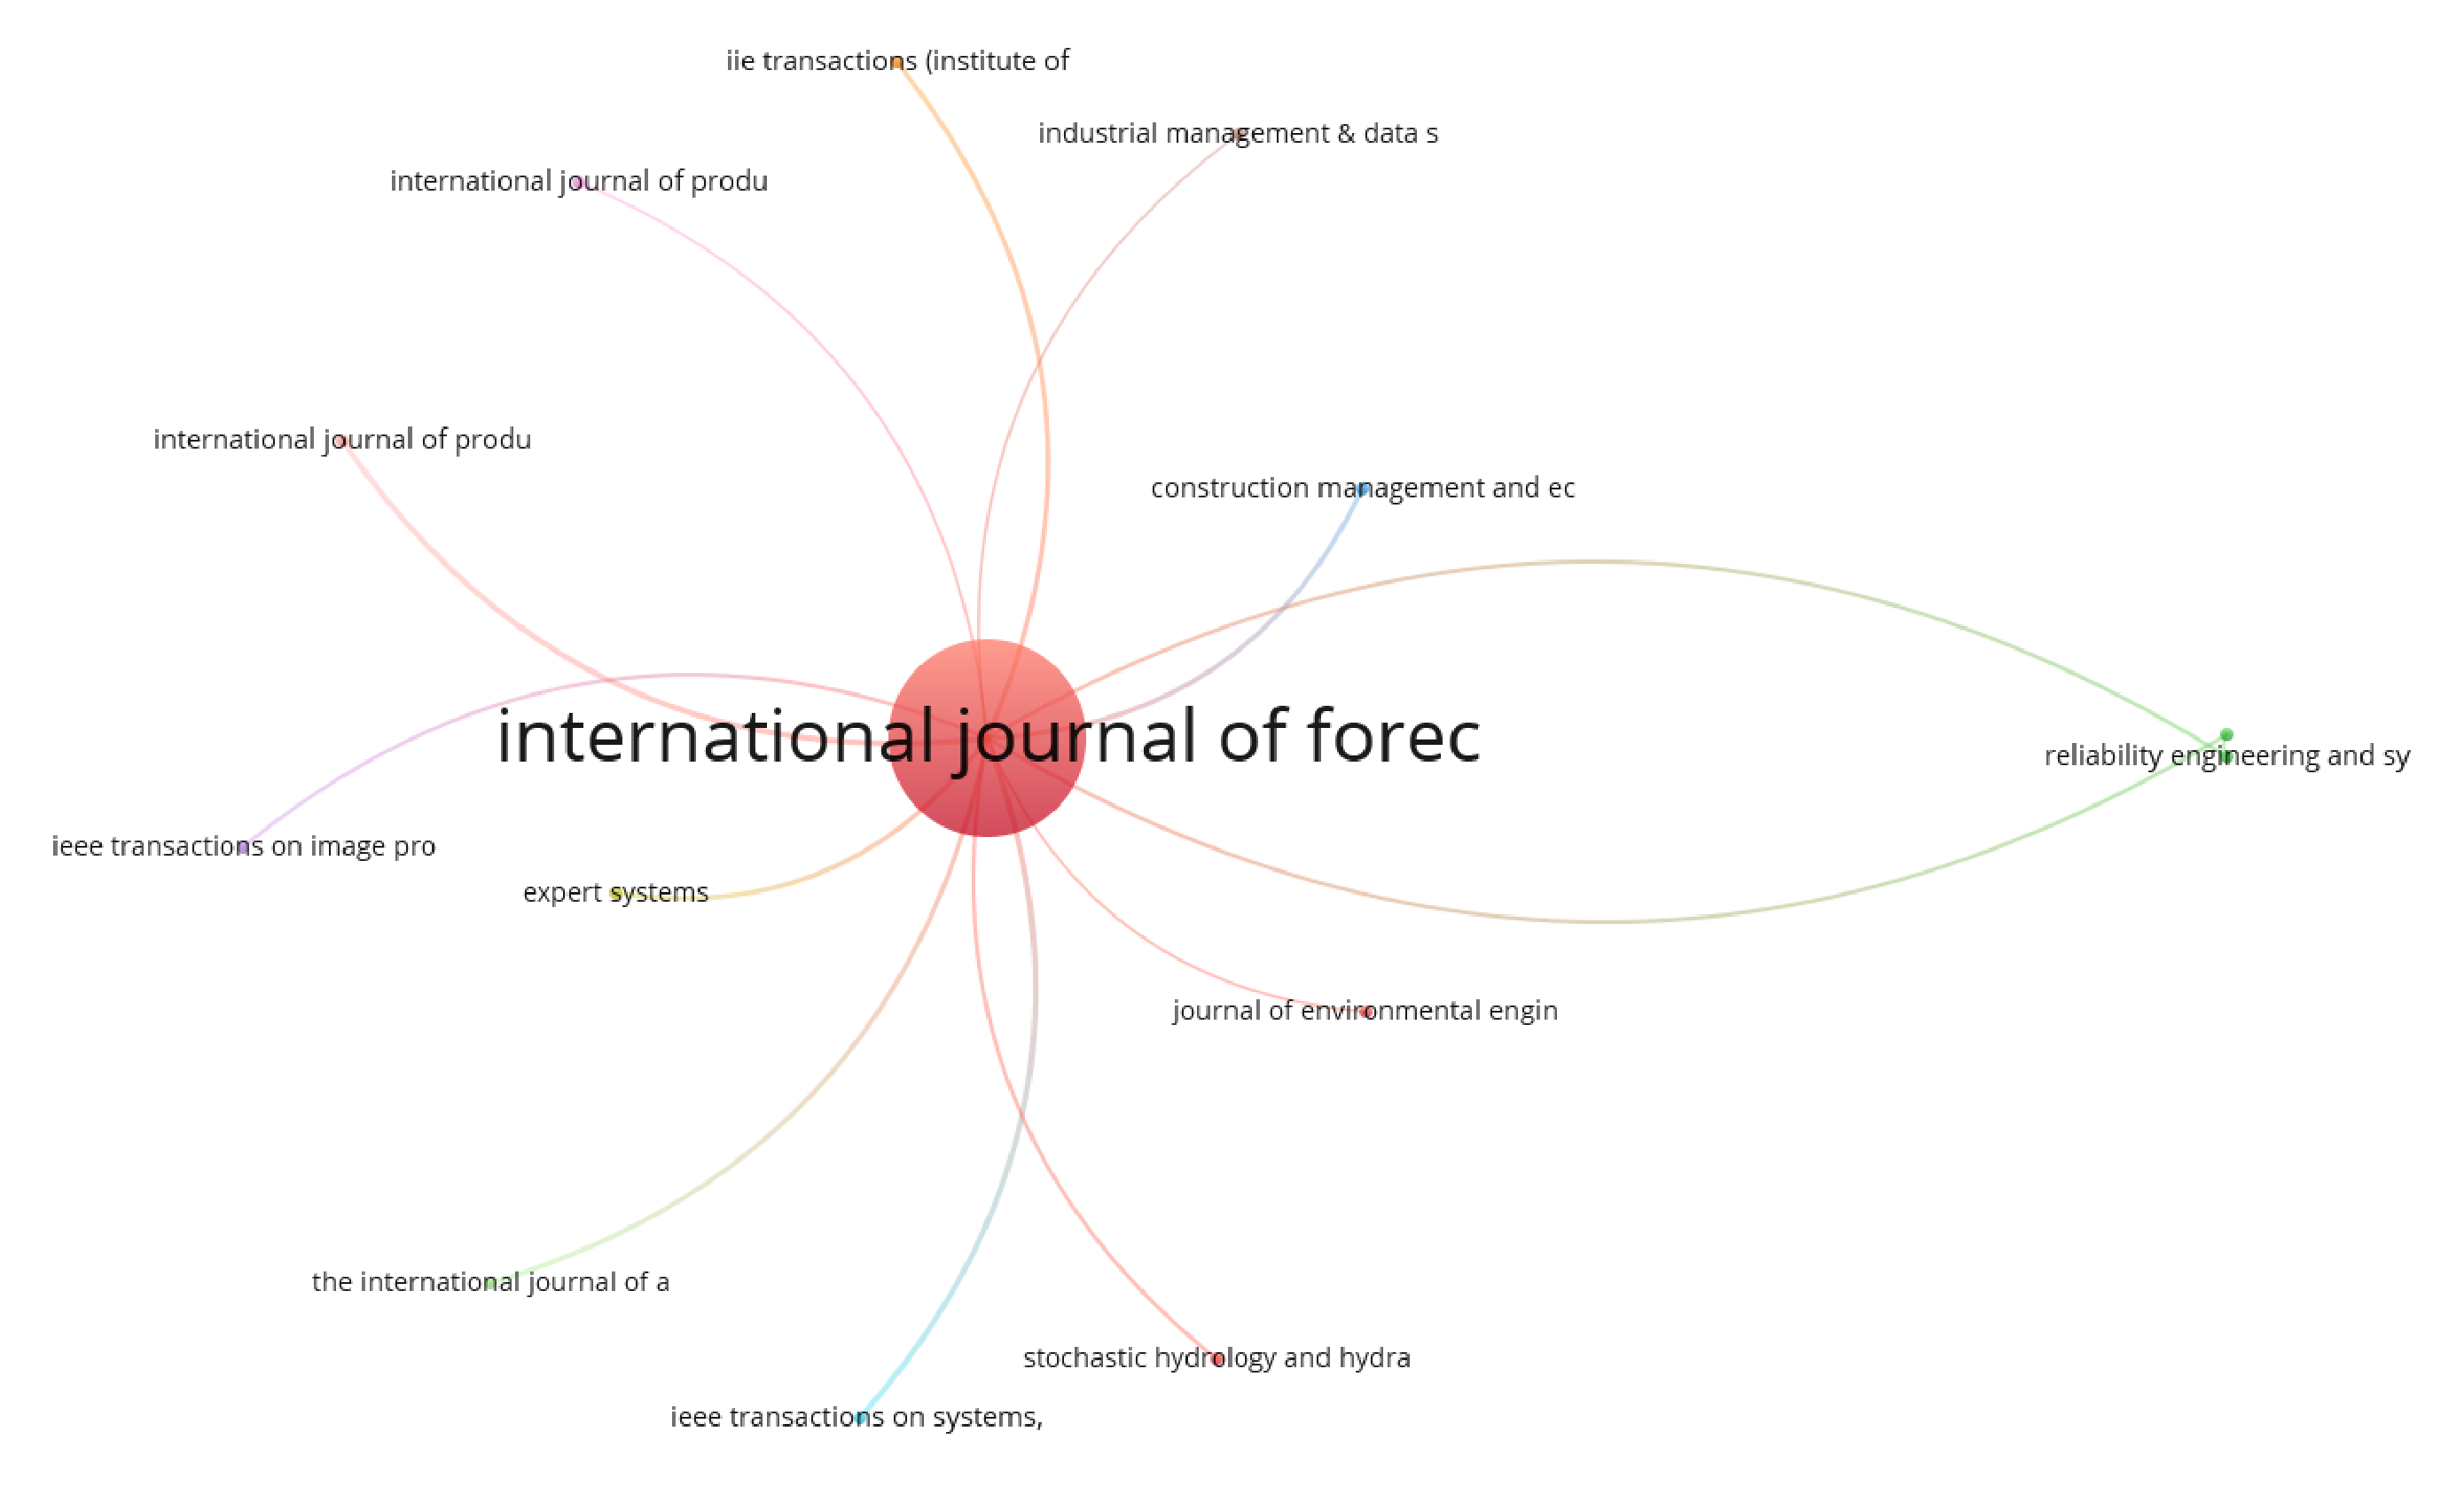
\includegraphics[scale=0.3]{fig.11.eps}
\caption{IJF Journal citation network in Engineering from 1985 to 1996}
\end{figure}

\begin{figure}[htbp]
\centering
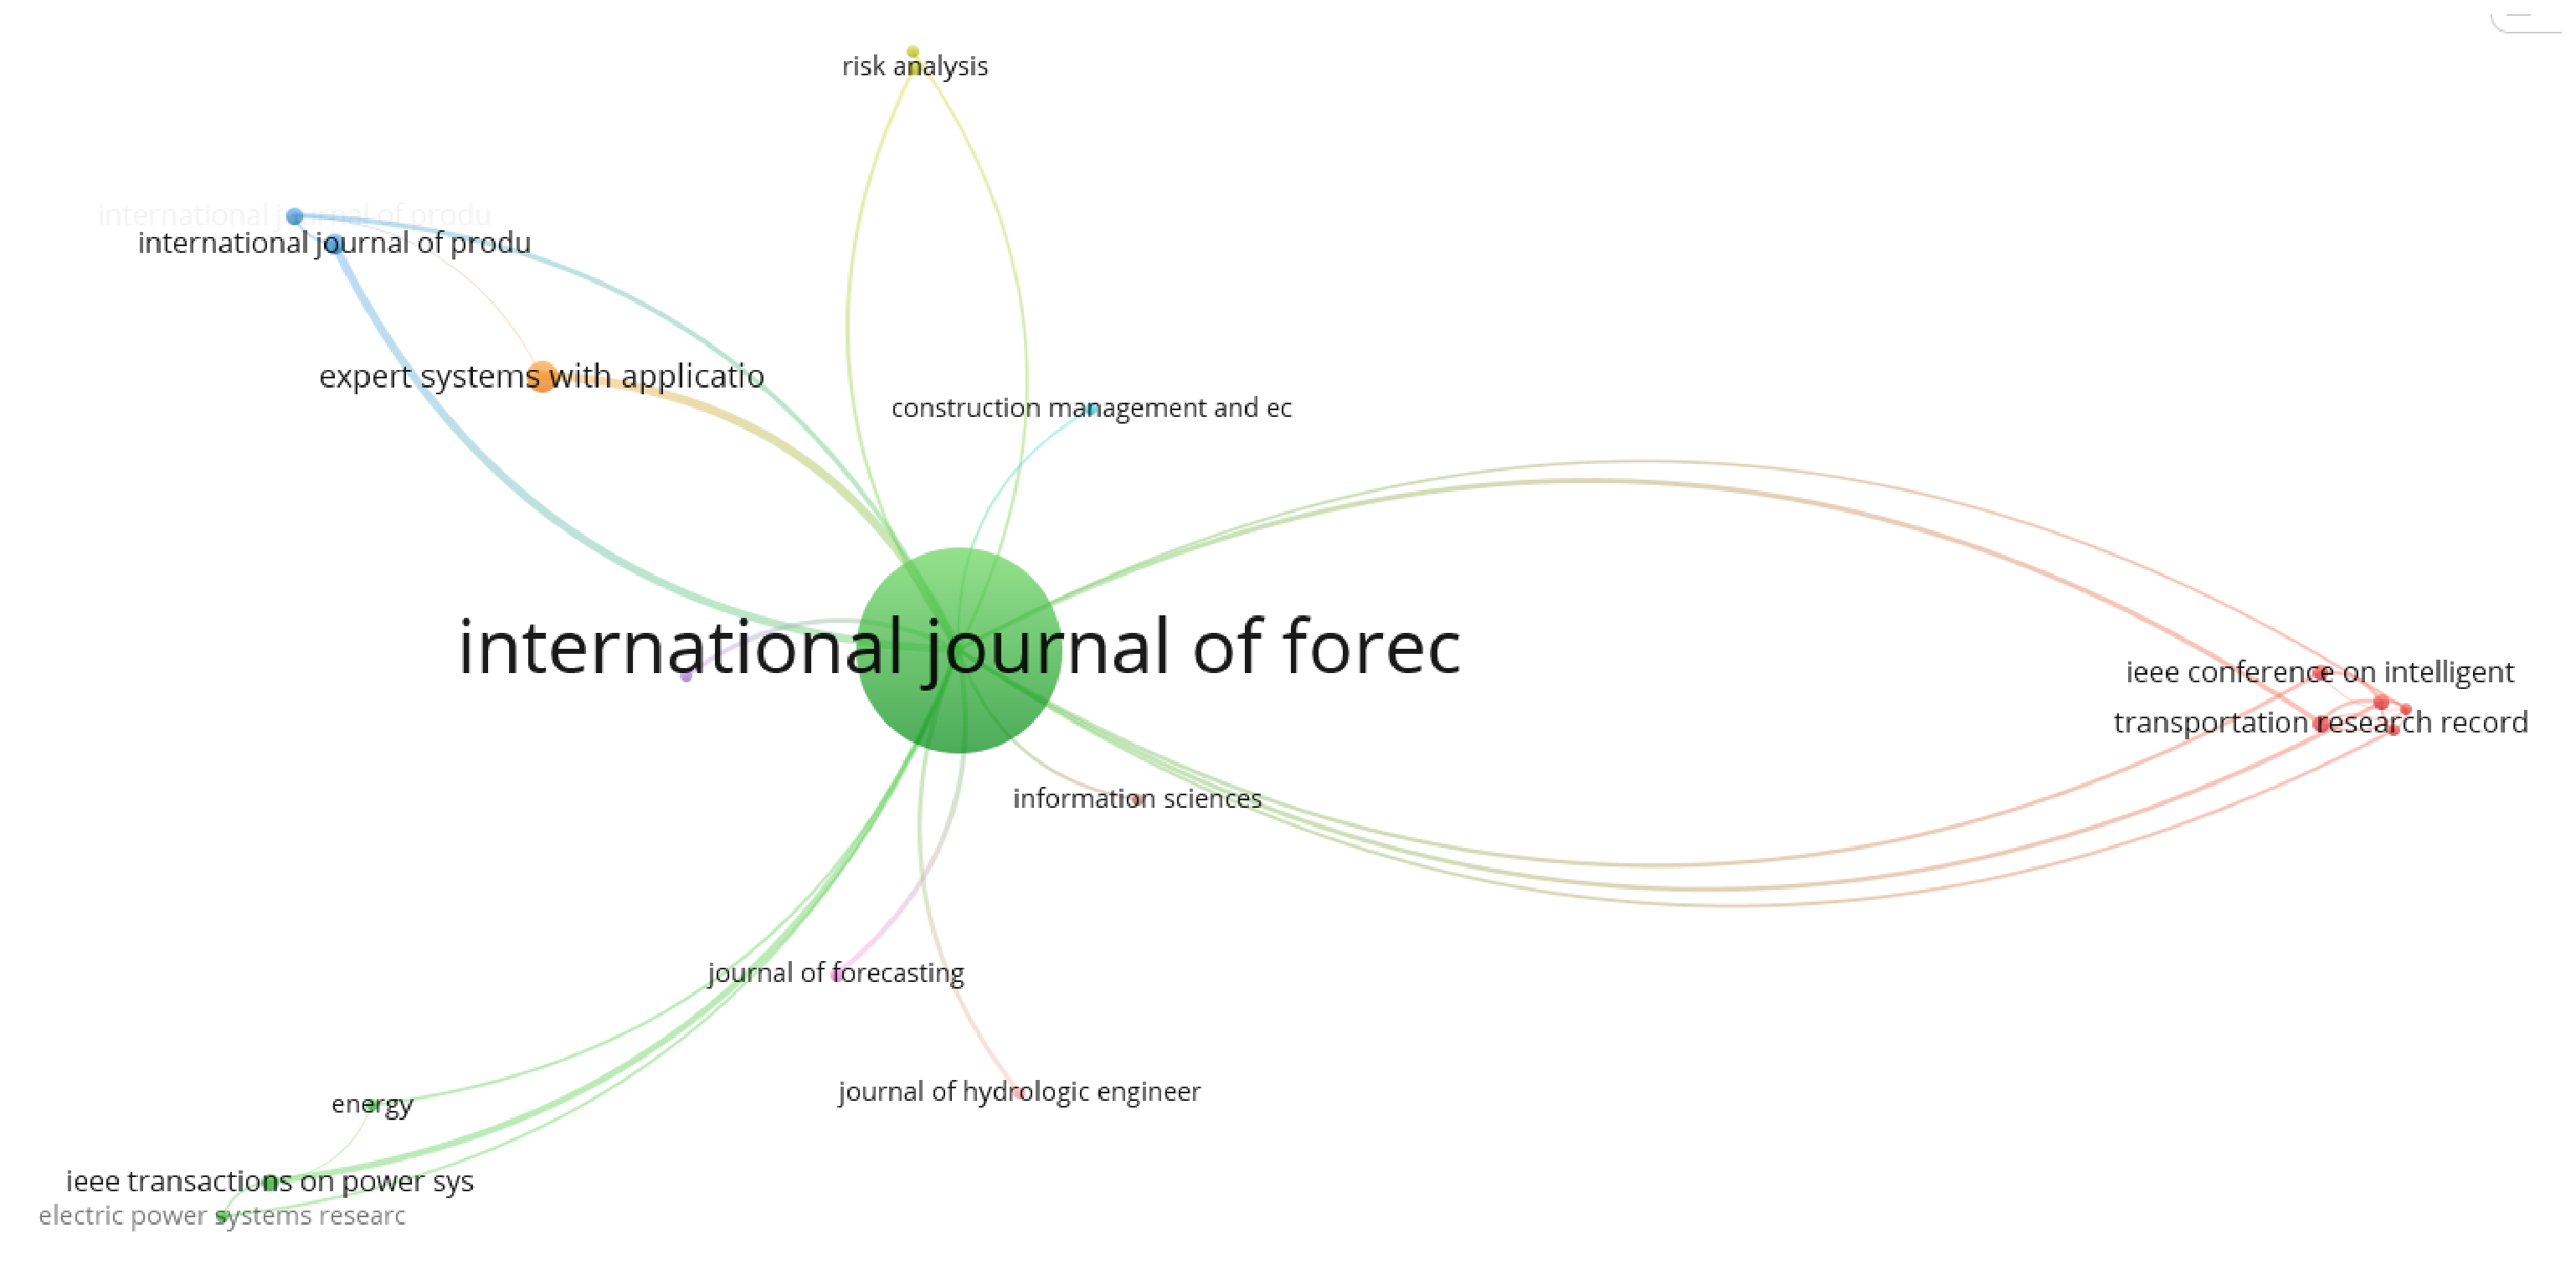
\includegraphics[scale=0.3]{fig.12.eps}
\caption{IJF Journal citation network in Engineering from 1997 to 2008}
\end{figure}

\begin{figure}[htbp]
\centering
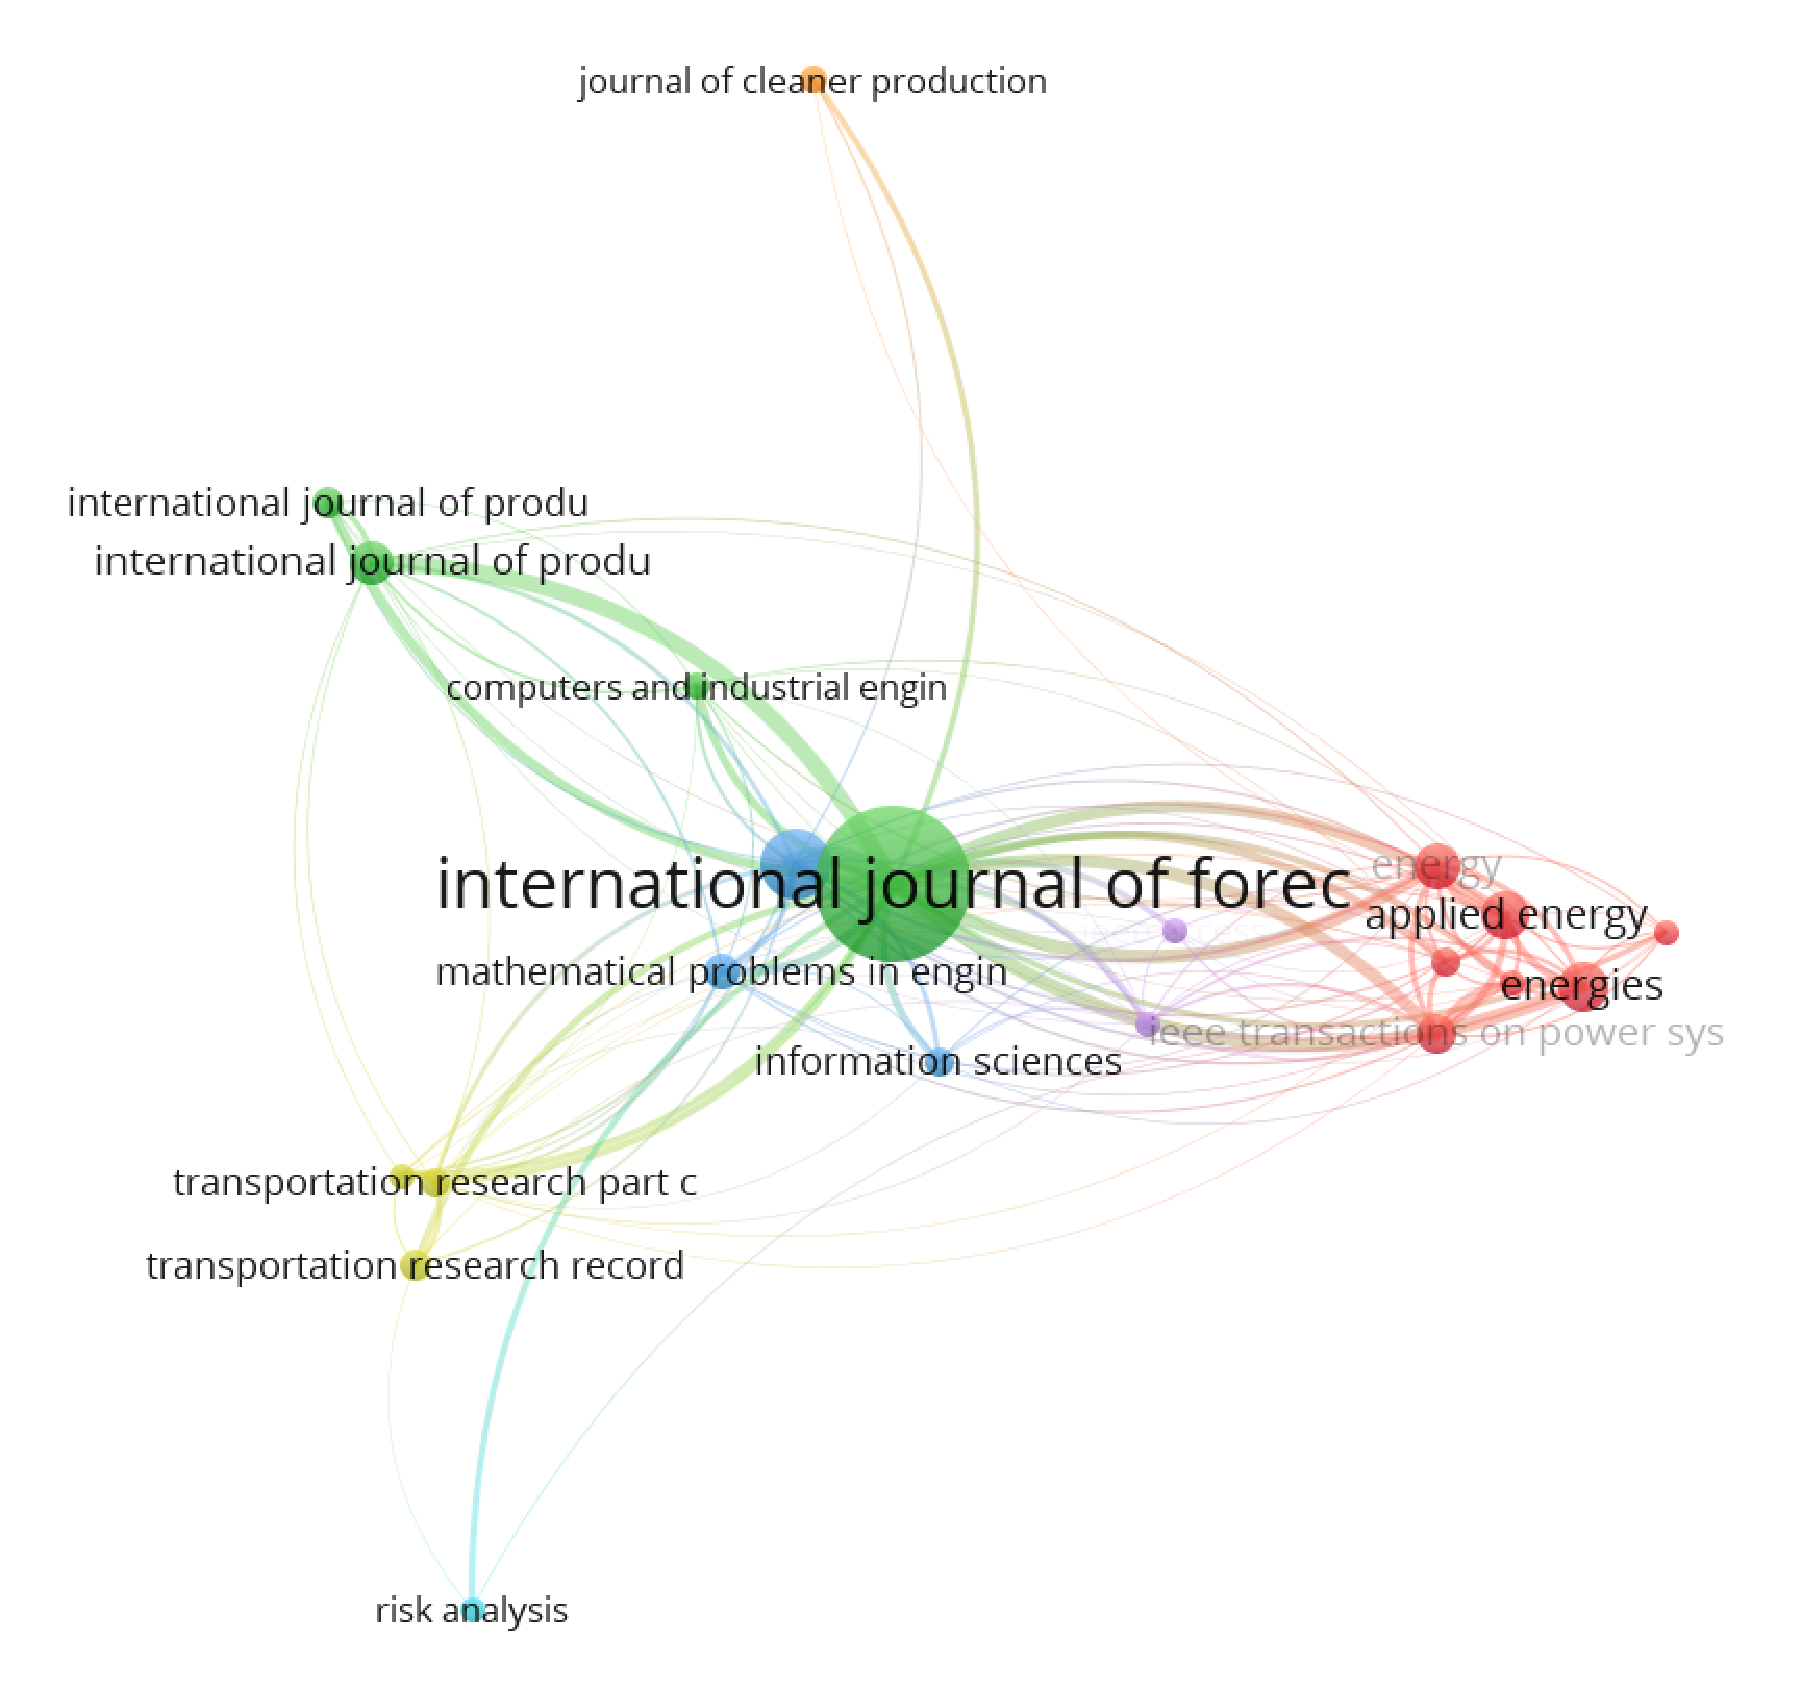
\includegraphics[scale=0.5]{fig.13.eps}
\caption{IJF Journal citation network in Engineering from 2009 to 2019}
\end{figure}

\begin{landscape}
\begin{table}[!htbp]
    \centering
    \caption{The information about the journal citation networks in Engineering based on the IJF citing papers}
    \setlength{\tabcolsep}{0.3mm}{
    \begin{tabular}{p{1.5cm}<{\centering} p{6cm}<{\centering} p{1.5cm}<{\centering}|p{1.5cm}<{\centering} p{6cm}<{\centering} p{1.5cm}<{\centering}|p{1.5cm}<{\centering} p{6cm}<{\centering} p{1.5cm}<{\centering}}
    \hline
        \hline
        \multicolumn{3}{c|}{1985-1996} & \multicolumn{3}{c|}{1997-2008} & \multicolumn{3}{c}{2009-2019}\\
    \hline
    \multicolumn{9}{c}{Limiting condition}\\
    \hline
        \multicolumn{3}{c|}{Number>=1 Citation>=10} & \multicolumn{3}{c|}{Number>=5 Citation>=200} & \multicolumn{3}{c}{Number>=40 Citation>=200}\\
    \hline
    \multicolumn{9}{c}{Parameters}\\
    \hline
    Clusters & Local links & Link strength & Clusters & Local links & Link strength & Clusters & Local links & Link strength\\
    9 & 18 & 173 & 8    & 66 & 1025 & 7 & 168 & 6146\\
        \hline
        \hline
   R & Journal & Links & R & Journal & Links & R & Journal & Links\\
   1 & IEEE Transactions on Systems, Man and Cybernetics & 4 & 1 & Expert Systems with Applications & 65 & 1 & Expert Systems with Applications & 520\\
   2 & International Journal of Production Research & 4 & 2 & International Journal of Production Economics & 53 & 2 & International Journal of Production Economics & 326\\
   3 & Construction Management and Economics & 3 & 3 & IEEE Transactions on Power Systems & 35 & 3 & Energies & 241\\
   4 & Expert Systems & 3 & 4 & Journal of Forecasting & 22 & 4 & Energy & 207\\
   5 & IIE Transactions & 3 & 5 & International Journal of Production Research & 20 & 5 & IEEE Transactions on Power Systems & 190\\
   6 & The International Journal of Advanced Manufacturing Technology & 3 & 6 & Transportation Research Record & 20 & 6 & Applied Energy & 167\\
   7 & IEEE Transactions on Engineering Management & 2 & 7 & Computers and Industrial Engineering & 18 & 7 & International Journal of Production Research & 106\\
   8 & IEEE Transactions on Image Processing & 2 & 8 & Journal of Hydrologic Engineering & 17 & 8 & Mathematical Problems in Engineering & 101\\
   9 & Reliability Engineering and System Safety & 2 & 9 & Transportation Research Part C: Emerging Technologies & 16 & 9 & International Journal of Electrical Power And Energy Systems & 81\\
   10 & Stochastic Hydrology and Hydraulics & 2 & 10 & IEEE Conference on Intelligent Transportation Systems & 13 & 10 & Computers and Industrial Engineering & 74\\
  \hline
  \hline
    \end{tabular}}
\end{table}
\end{landscape}

\noindent 3.2.1.3. Journal citation network in Decision Science

The journal citation relationships based on the IJF papers and citing
papers belonging to Decision Science are depicted in the Fig. 14-16, and
the detailed information is stated in table 14. IJF is an absolute
center in three networks, and JF is always the most citing journal. In
Decision Science, almost all of the top journals in period 1 appear in
period 2 or 3, which means the compositions of three journal citation
networks are much stable over time. Observing from Fig. 16, there are
three main clusters connected to IJF in the last ten years, which are
operational research related journals, statistics related journals, and
decision making related journals. Naturally, in the range of Decision
Science, these three kinds of journals are the most royal audiences to
the IJF researches in recent time.

\begin{figure}[htbp]
\centering
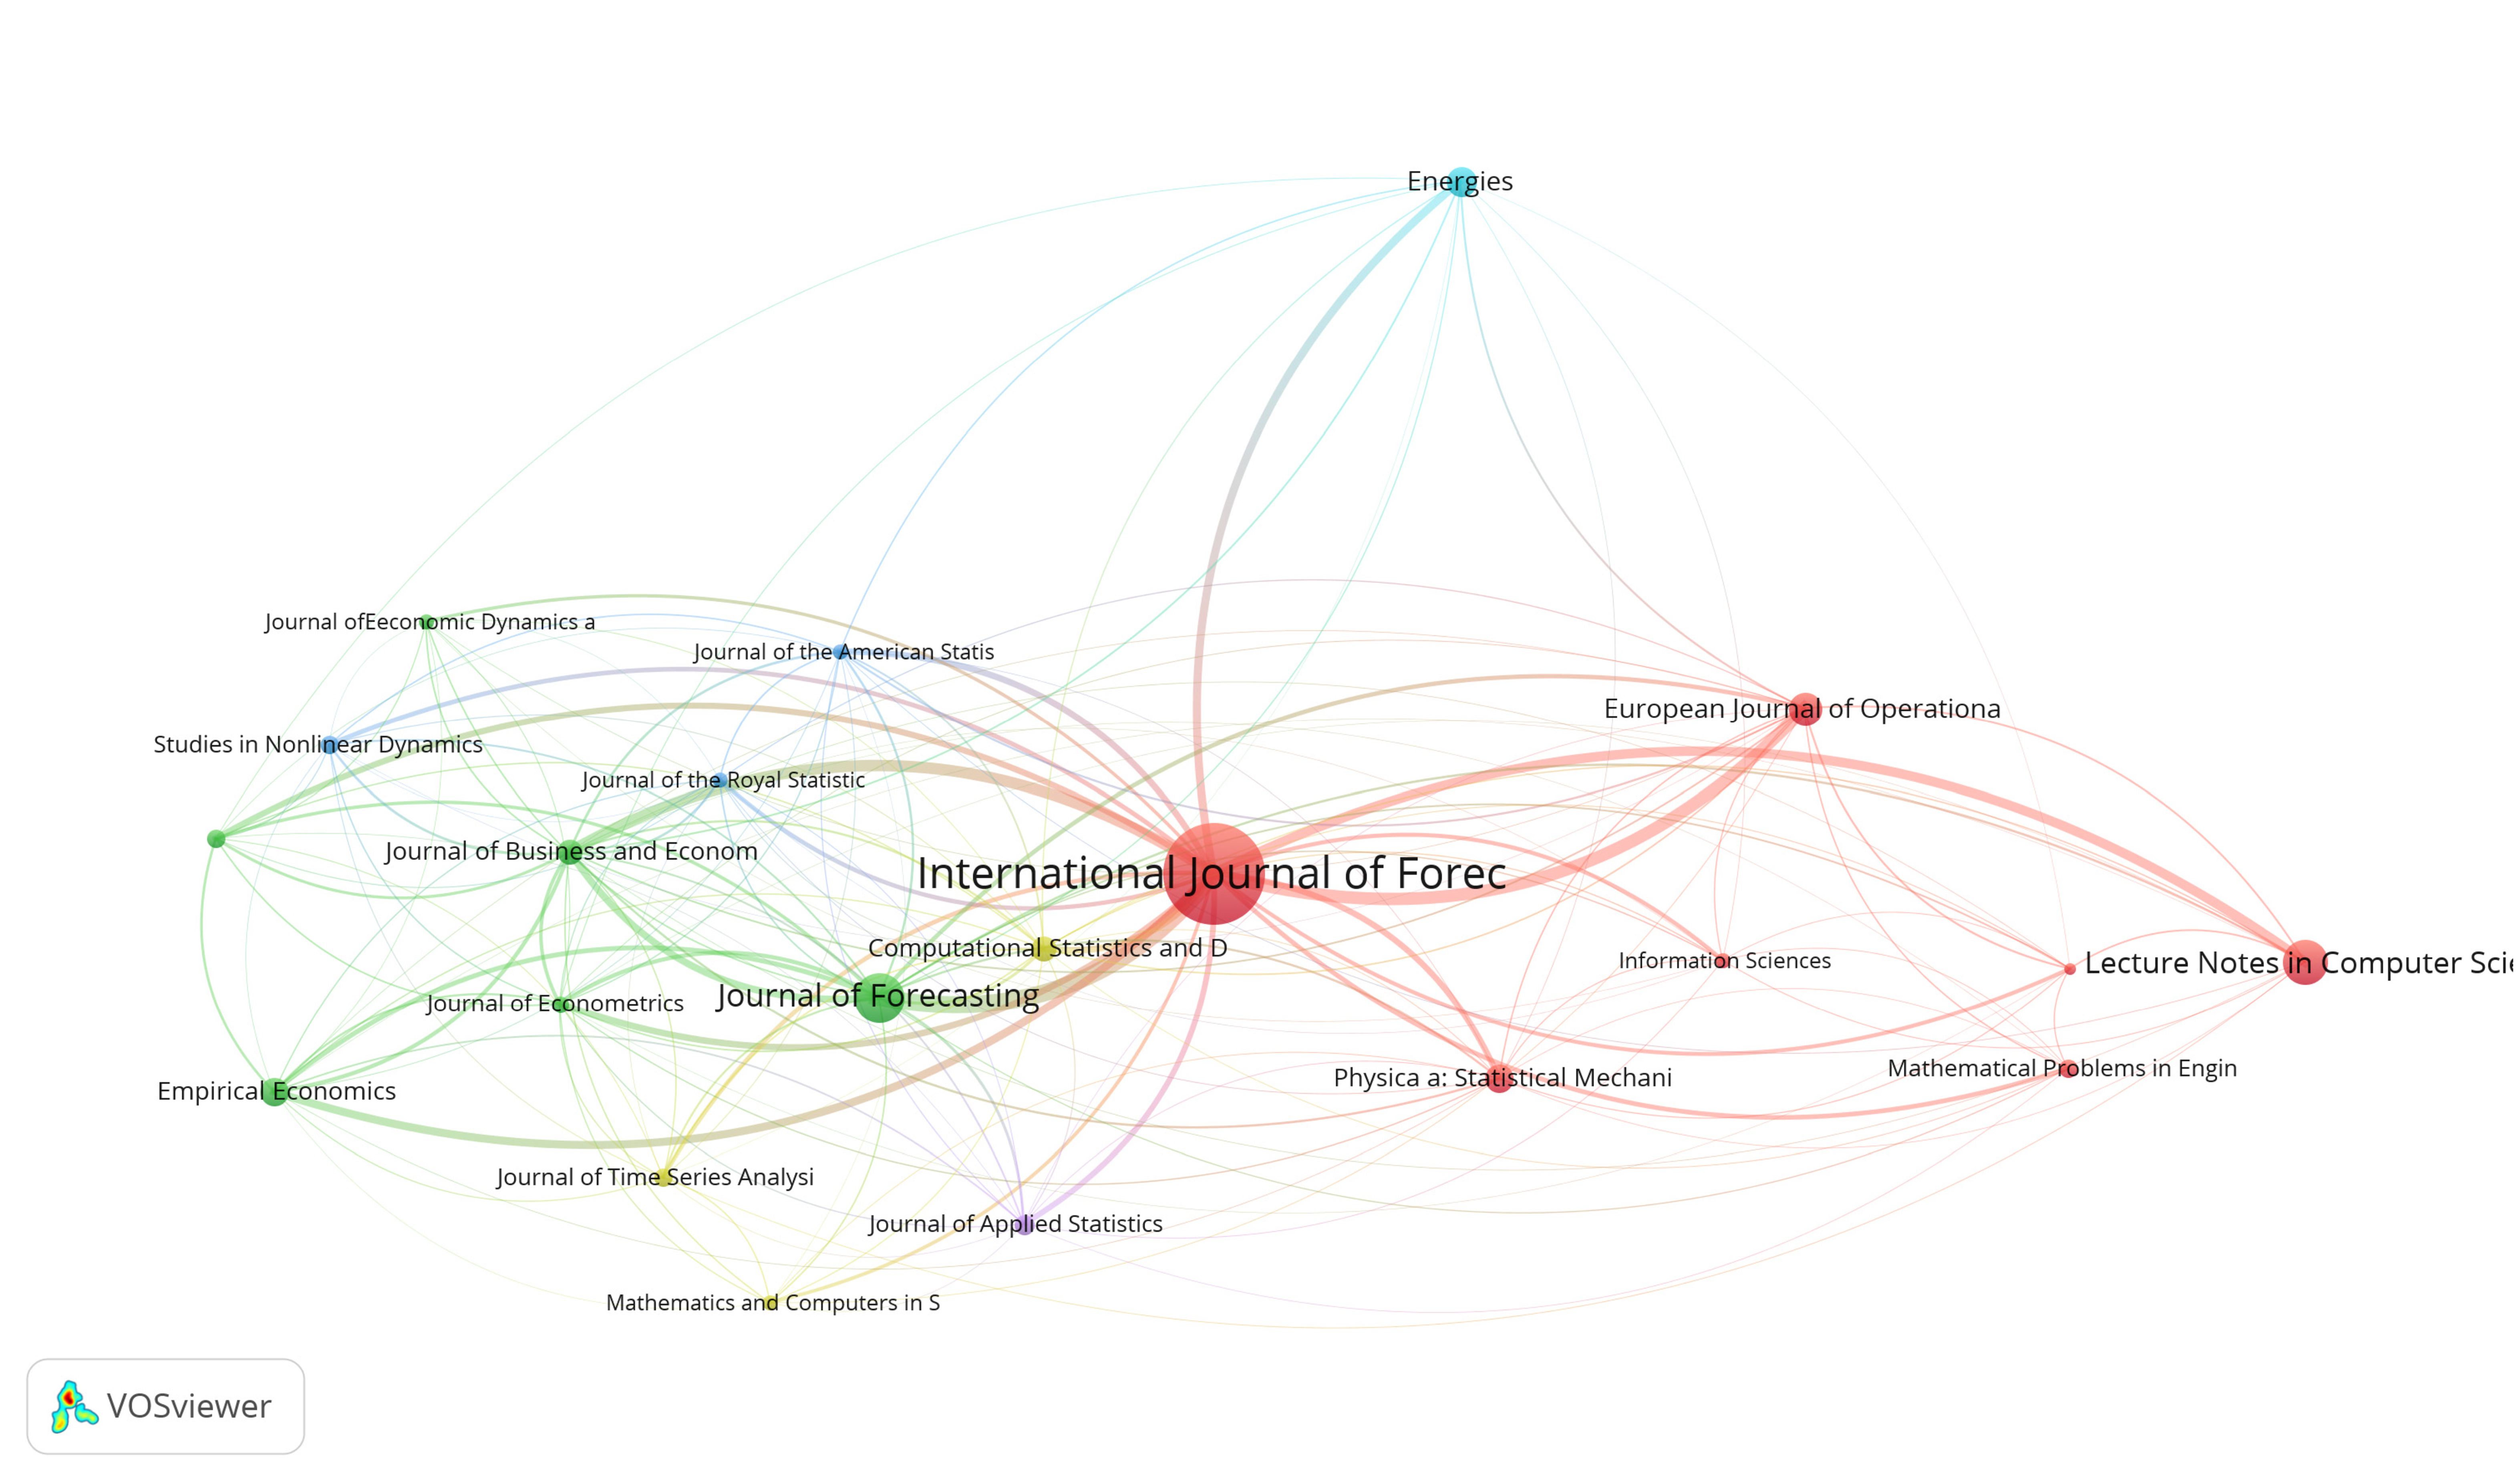
\includegraphics[scale=0.4]{fig.14.eps}
\caption{IJF Journal citation network in Decision Science from 1985 to 1996}
\end{figure}

\begin{figure}[htbp]
\centering
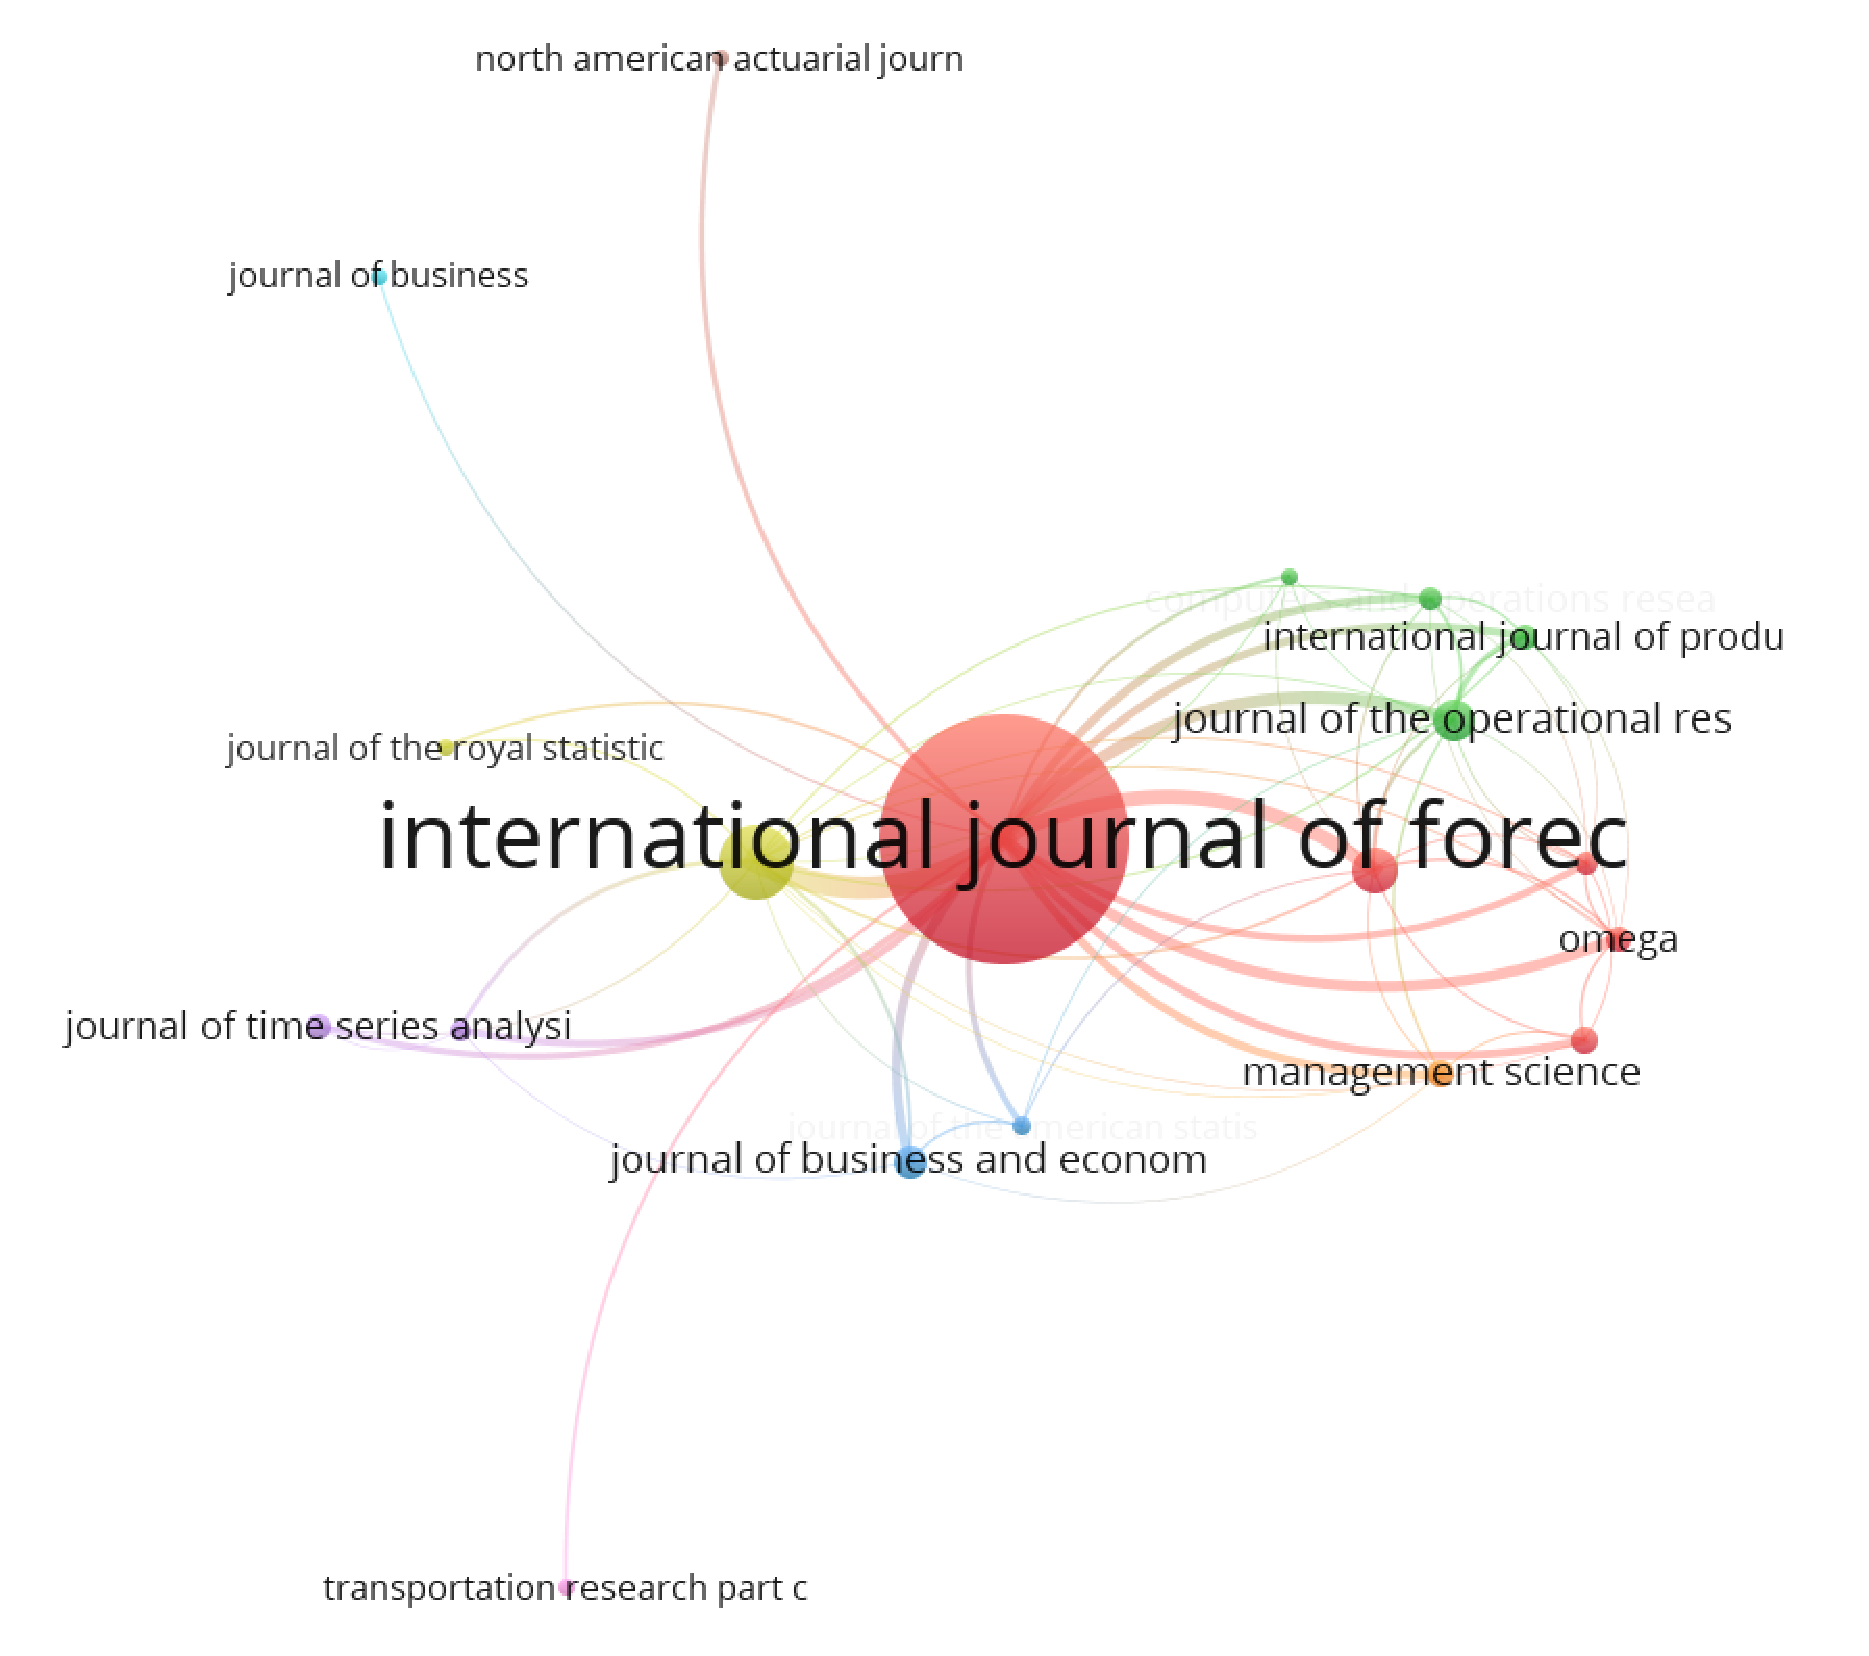
\includegraphics[scale=0.4]{fig.15.eps}
\caption{IJF Journal citation network in Decision Science from 1997 to 2008}
\end{figure}

\begin{figure}[htbp]
\centering
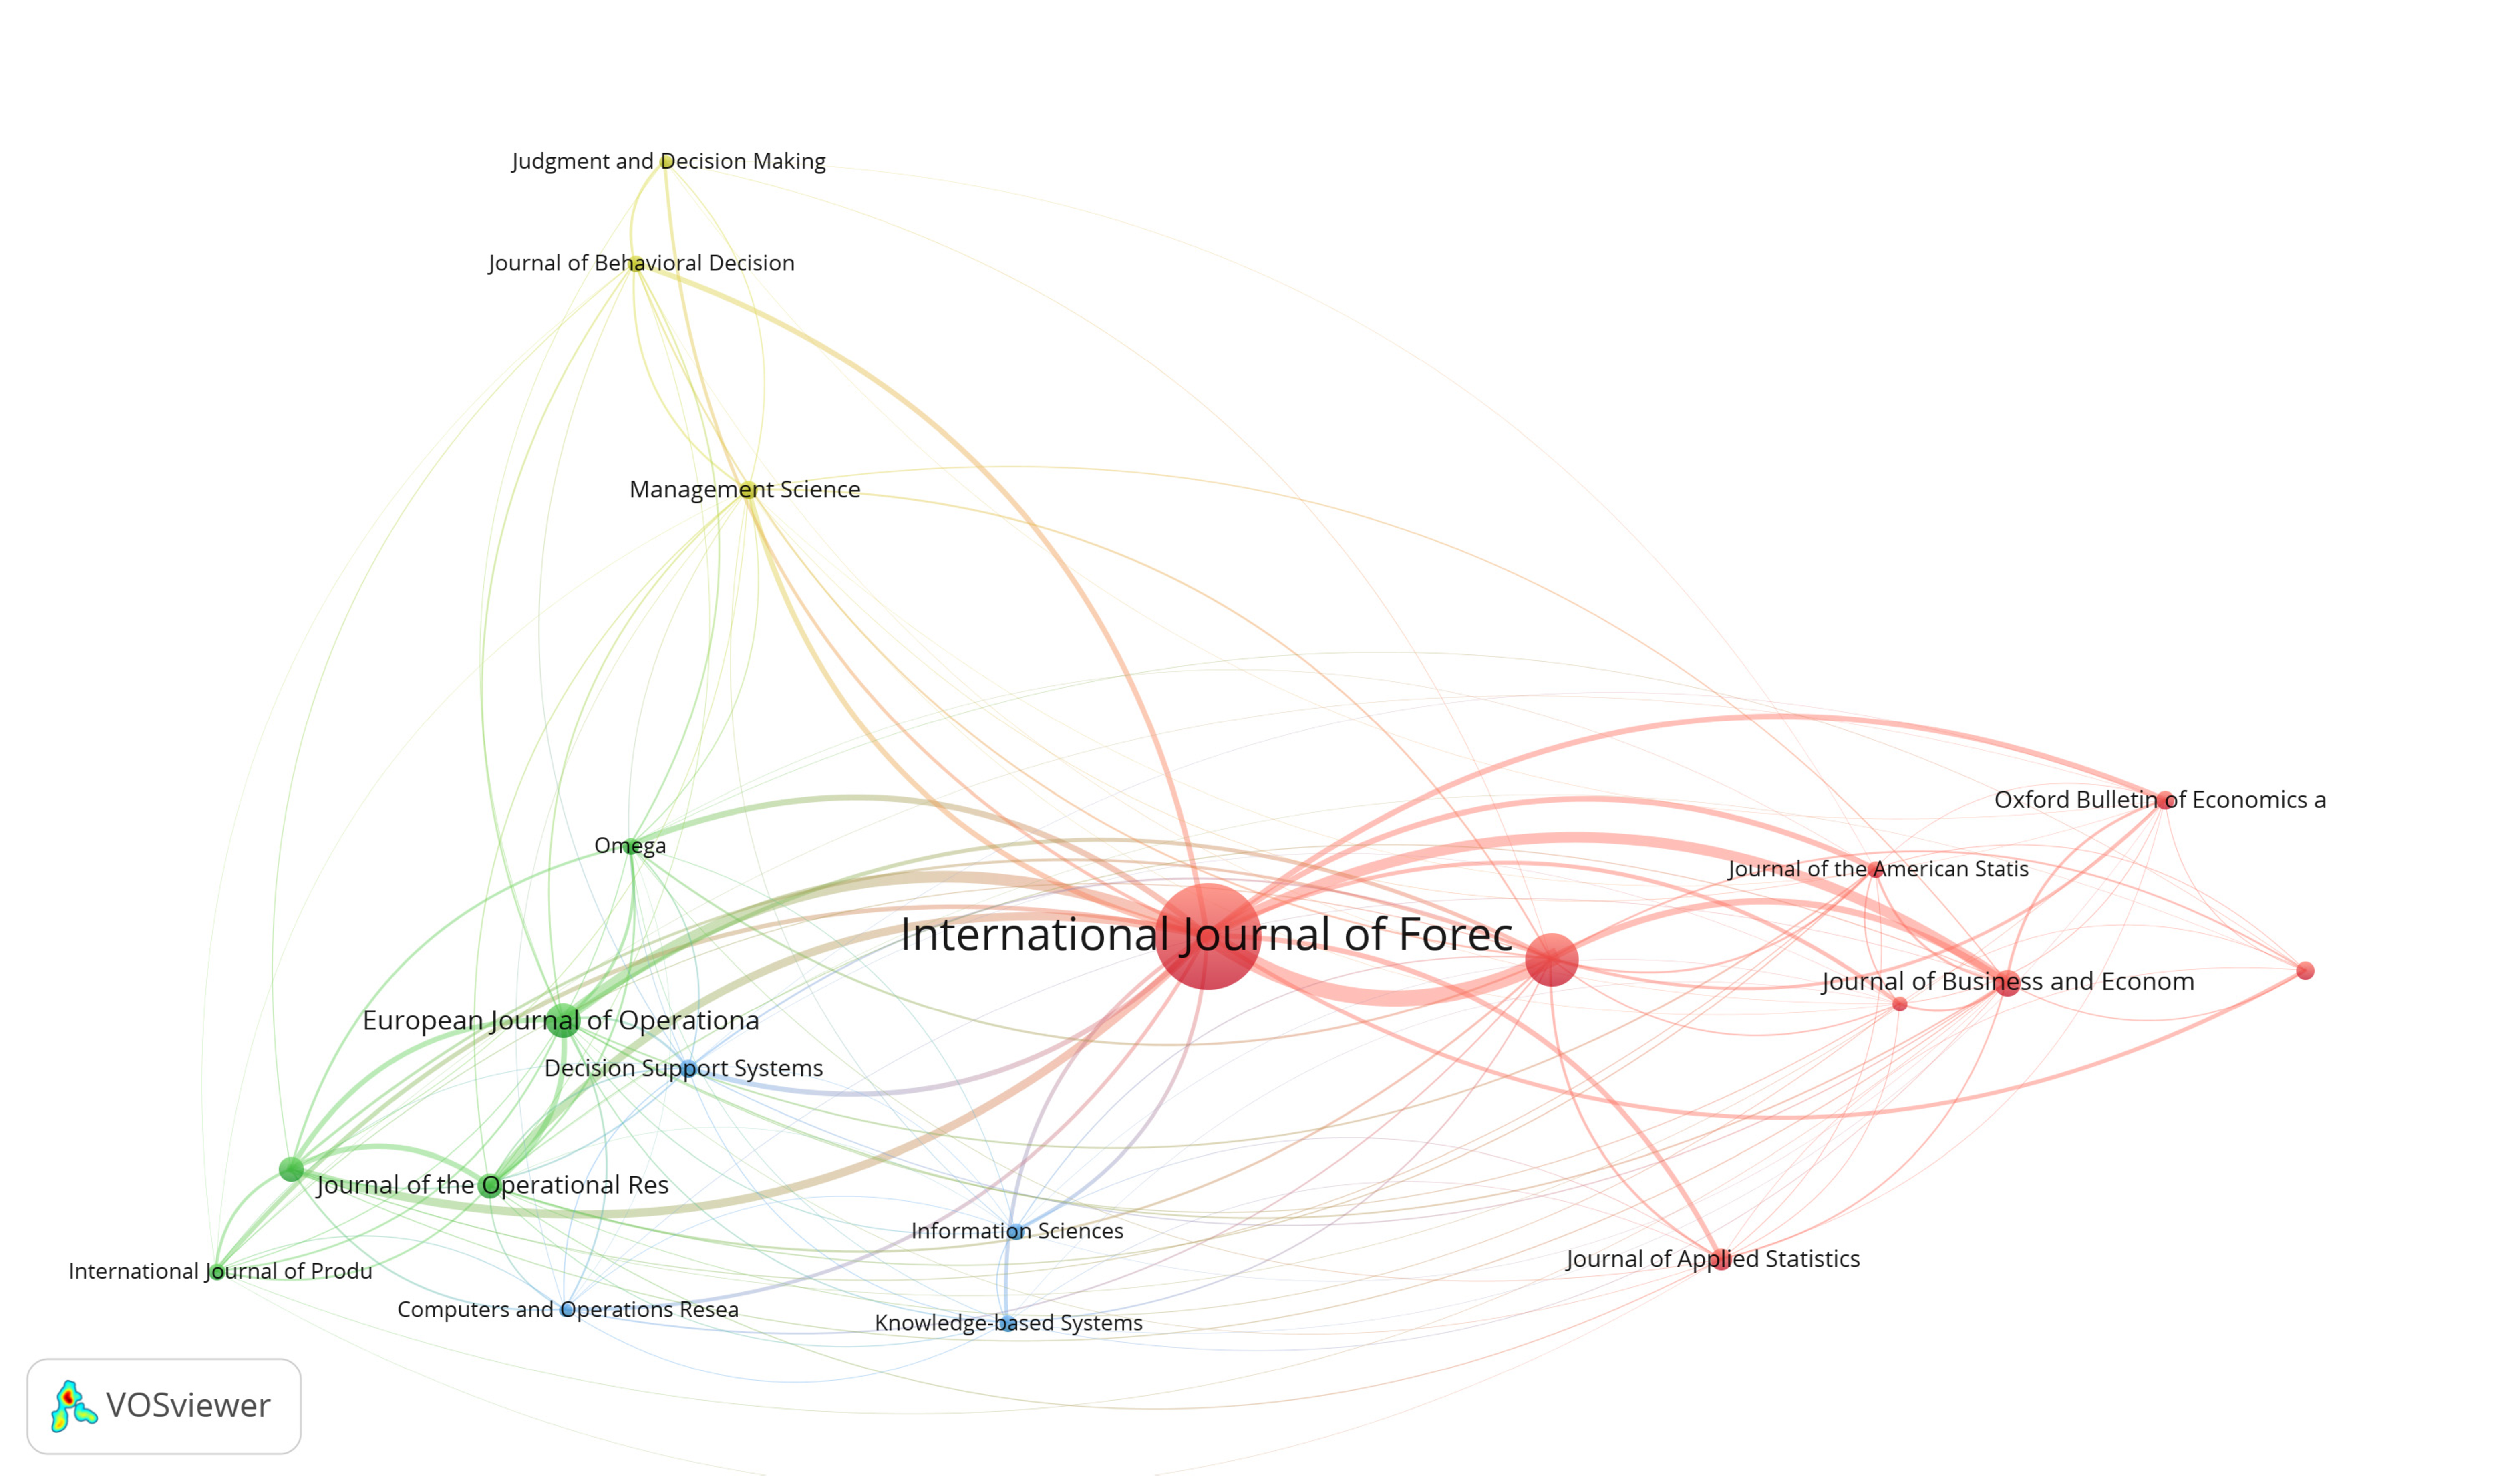
\includegraphics[scale=0.3]{fig.16.eps}
\caption{IJF Journal citation network in Decision Science from 2009 to 2019 }
\end{figure}

\begin{landscape}
\begin{table}[!htbp]
    \centering
    \caption{The information about the journal citation networks in Decision Science based on the IJF citing papers}
    \setlength{\tabcolsep}{0.3mm}{
    \begin{tabular}{p{1.5cm}<{\centering} p{6cm}<{\centering} p{1.5cm}<{\centering}|p{1.5cm}<{\centering} p{6cm}<{\centering} p{1.5cm}<{\centering}|p{1.5cm}<{\centering} p{6cm}<{\centering} p{1.5cm}<{\centering}}
    \hline
        \hline
        \multicolumn{3}{c|}{1985-1996} & \multicolumn{3}{c|}{1997-2008} & \multicolumn{3}{c}{2009-2019}\\
    \hline
    \multicolumn{9}{c}{Limiting condition}\\
    \hline
        \multicolumn{3}{c|}{Number>=1 Citation>=10} & \multicolumn{3}{c|}{Number>=5 Citation>=200} & \multicolumn{3}{c}{Number>=40 Citation>=200}\\
    \hline
    \multicolumn{9}{c}{Parameters}\\
    \hline
    Clusters & Local links & Link strength & Clusters & Local links & Link strength & Clusters & Local links & Link strength\\
    9 & 18 & 173 & 8    & 66 & 1025 & 7 & 168 & 6146\\
        \hline
        \hline
   R & Journal & Links & R & Journal & Links & R & Journal & Links\\
1 & Journal of Forecasting & 139 & 1 & Journal of Forecasting & 365 & 1 & Journal of Forecasting & 1448\\
2 & Journal of Behavioral Decision Making & 24 & 2 & European Journal of Operational Research & 152 & 2 & European Journal of Operational Research & 721\\
3 & Journal of Business and Economic Statistics & 23 & 3 & Journal of the Operational Research Society & 117 & 3 & Journal of Business and Economic Statistics & 625\\
4 & Journal of The Operational Research Society & 15 & 4 & Omega & 88 & 4 & International Journal of Production Economics & 394\\
5 & Journal of the American Statistical Association & 14 & 5 & Journal of Business and Economic Statistics & 64 & 5 & Journal of the Operational Research Society & 353\\
6 & Omega & 13 & 6 & Computers and Operations Research & 54 & 6 & Omega & 205\\
7 & Journal of Applied Statistics & 10 & 7 & Management Science & 49 & 7 & Journal of the American Statistical Association & 182\\
8 & Decision Sciences & 9 & 8 & Journal of Behavioral Decision Making & 48 & 8 & Oxford Bulletin of Economics And Statistics & 179\\
9 & European Journal of Operational Research & 8 & 9 & International Journal of Production Economics & 47 & 9 & Journal of Behavioral Decision Making & 162\\
10 & Decision Support Systems & 6 & 10 & Decision Support Systems & 39 & 10 & Management Science & 159\\
  \hline
  \hline
    \end{tabular}}
\end{table}
\end{landscape}

\noindent 3.2.1.4. Journal citation network in Psychology

Citing papers belonging to Psychology are much less than those belonging
to other three subject areas, but the compositions of top four journals
in Psychology over time are the most stable comparing with other three
subject areas. Organizational Behavior and Human Decision Processes,
Journal of Behavioral Decision Making, Decision Support Systems, and
Technological Forecasting and Social Change are top four journals in
period 1, 2 and 3, which means in Psychology they are most interested in
IJF researches than other journals. However, except for the top four
journals, the remaining journals changed a lot over time, which
demonstrates in Psychology, IJF attracts different non-primary journals
in different periods.

\begin{figure}[htbp]
\centering
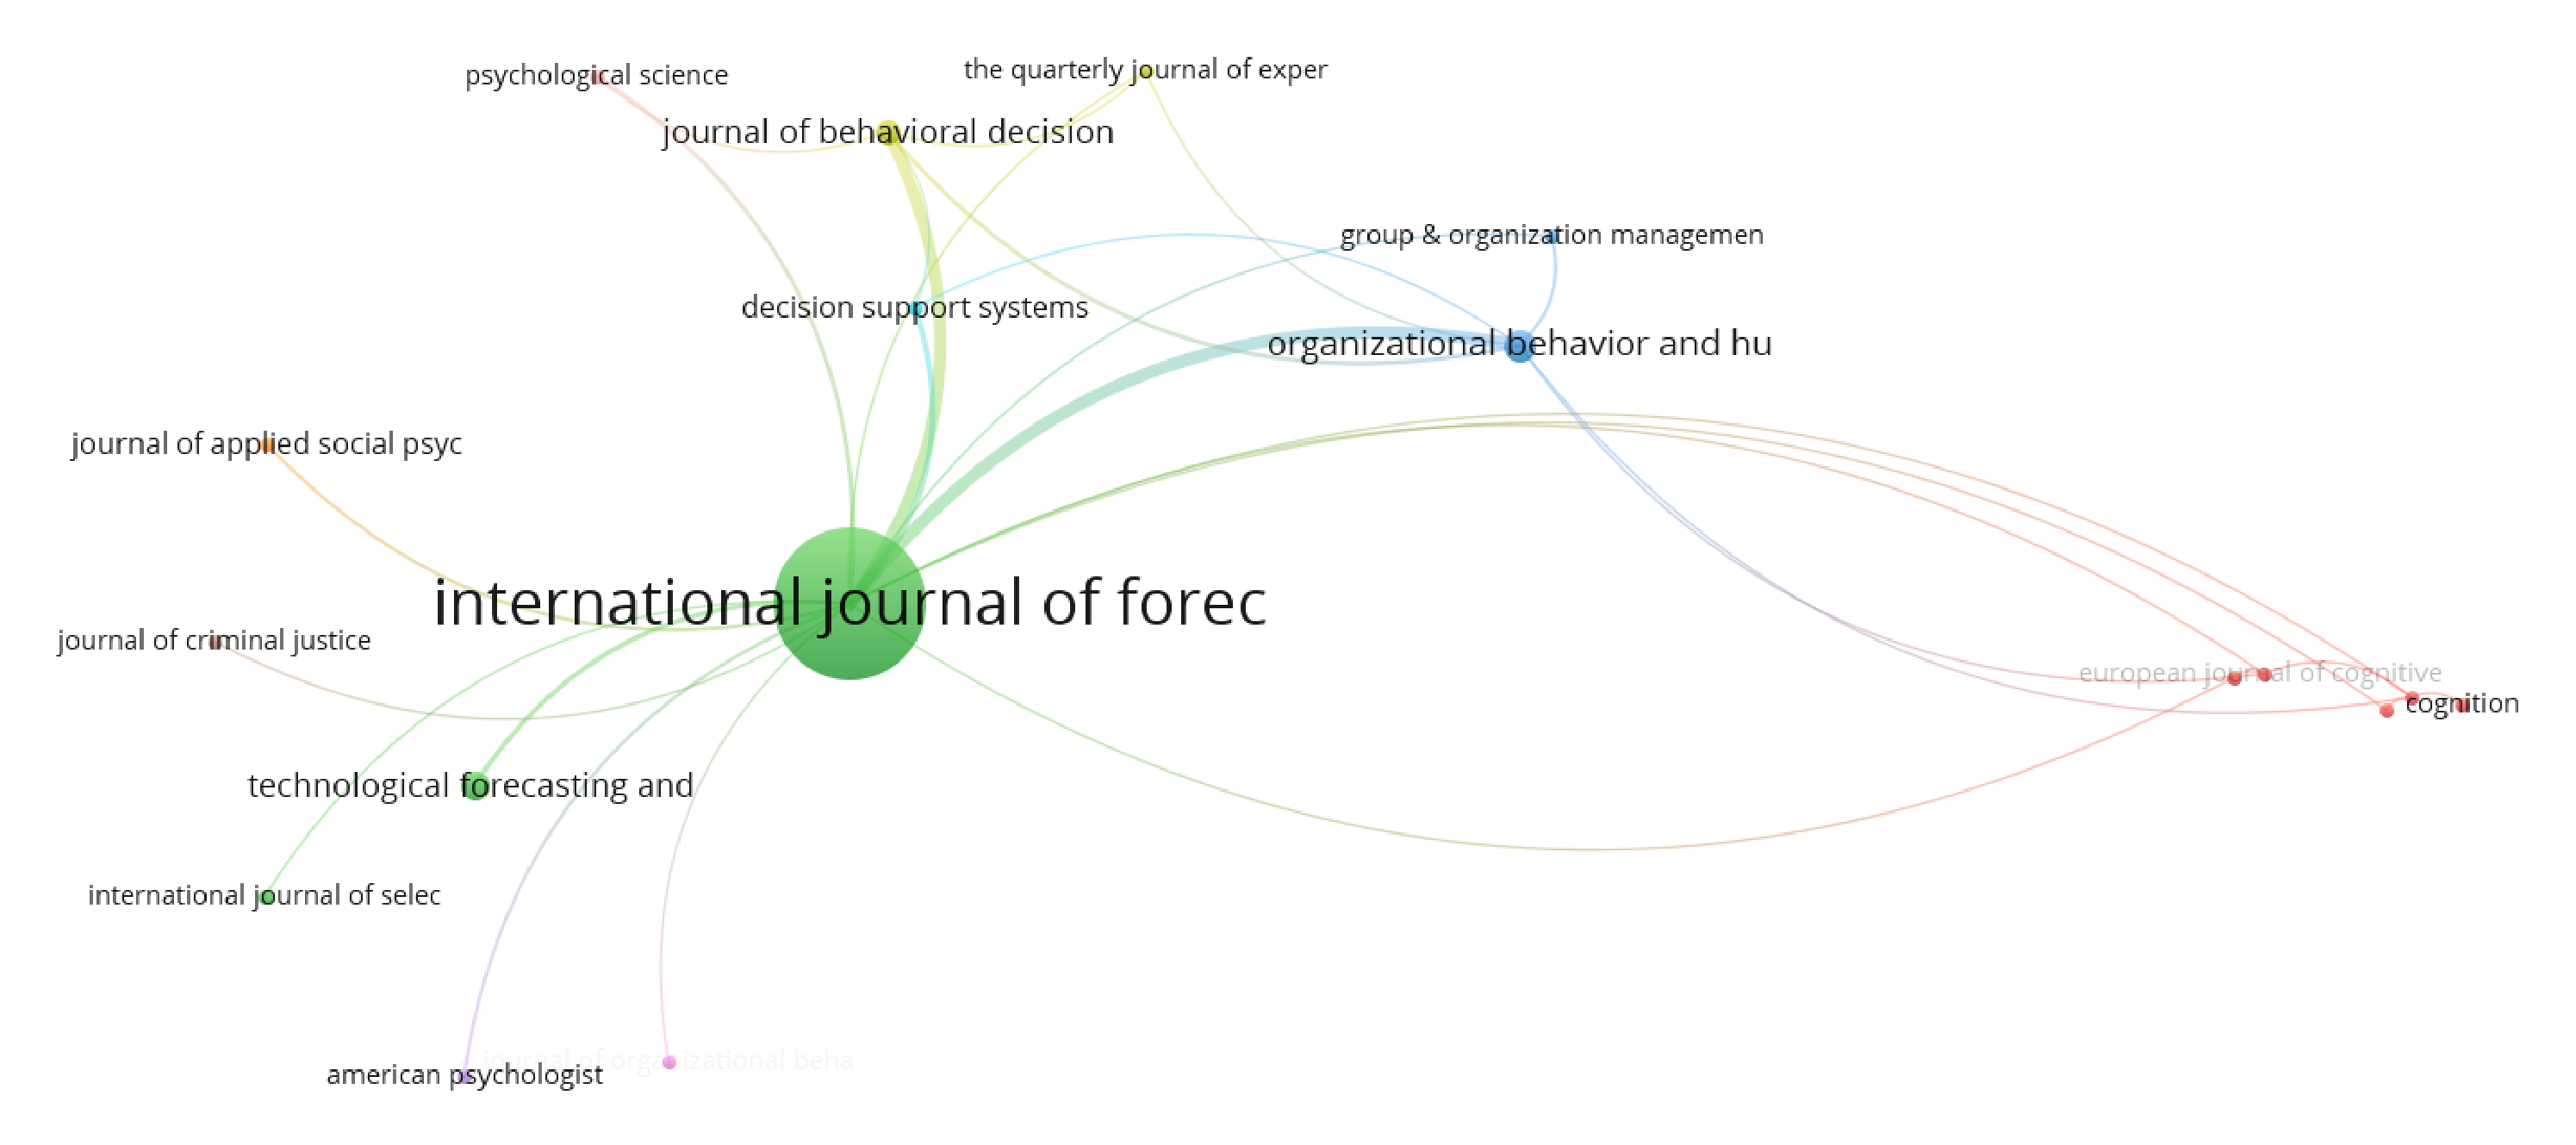
\includegraphics[scale=0.3]{fig.17.eps}
\caption{ IJF Journal citation network in Psychology from 1985 to 1996}
\end{figure}

\begin{figure}[htbp]
\centering

\includegraphics[scale=0.3]{fig.18.eps}
\caption{IJF Journal citation network in Psychology from 1997 to 2008}
\end{figure}

\begin{figure}[htbp]
\centering
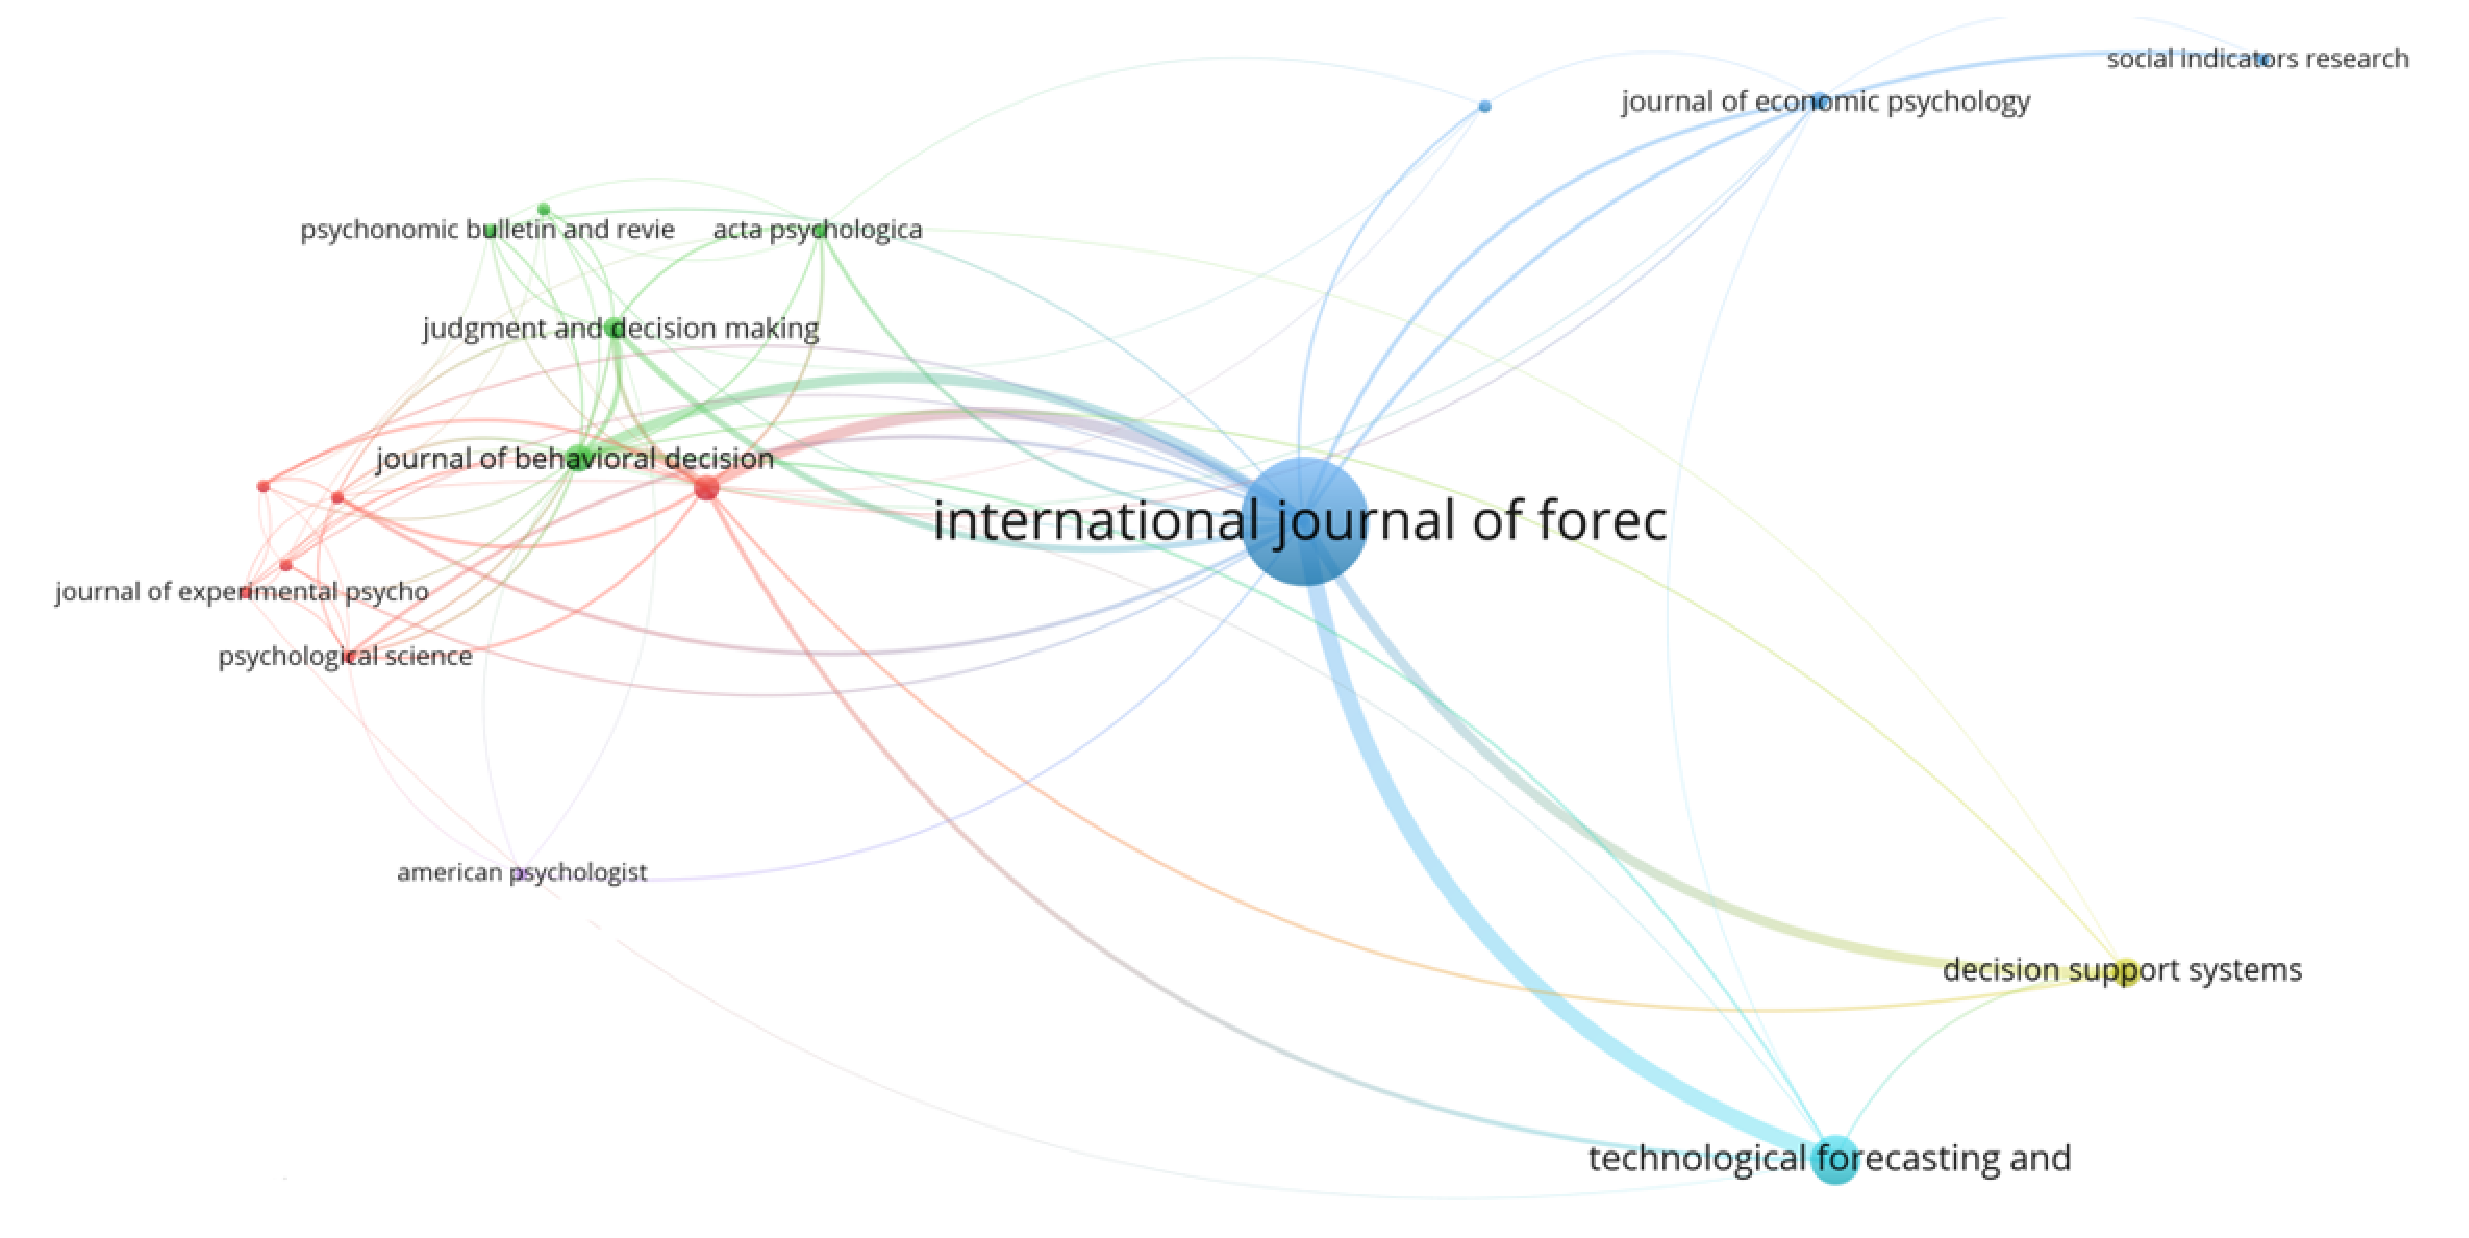
\includegraphics[scale=0.3]{fig.19.eps}
\caption{IJF Journal citation network in Psychology from 2009 to 2019}
\end{figure}

\begin{landscape}
\begin{table}[!htbp]
    \centering
    \caption{The information about the journal citation networks in Psychology based on the IJF citing papers}
    \setlength{\tabcolsep}{0.3mm}{
    \begin{tabular}{p{1.5cm}<{\centering} p{6cm}<{\centering} p{1.5cm}<{\centering}|p{1.5cm}<{\centering} p{6cm}<{\centering} p{1.5cm}<{\centering}|p{1.5cm}<{\centering} p{6cm}<{\centering} p{1.5cm}<{\centering}}
    \hline
        \hline
        \multicolumn{3}{c|}{1985-1996} & \multicolumn{3}{c|}{1997-2008} & \multicolumn{3}{c}{2009-2019}\\
    \hline
    \multicolumn{9}{c}{Limiting condition}\\
    \hline
        \multicolumn{3}{c|}{Number>=1 Citation>=10} & \multicolumn{3}{c|}{Number>=5 Citation>=200} & \multicolumn{3}{c}{Number>=40 Citation>=200}\\
    \hline
    \multicolumn{9}{c}{Parameters}\\
    \hline
    Clusters & Local links & Link strength & Clusters & Local links & Link strength & Clusters & Local links & Link strength\\
    9 & 18 & 173 & 8    & 66 & 1025 & 7 & 168 & 6146\\
  \hline
  \hline
   R & Journal & Links & R & Journal & Links & R & Journal & Links\\
   1 & Organizational Behavior and Human Decision Processes & 27 & 1 & Organizational Behavior and Human Decision Processes & 54 & 1 & Technological Forecasting and Social Change & 425\\
   2 & Journal of Behavioral Decision Making & 24 & 2 & Journal of Behavioral Decision Making & 48 & 2 & Organizational Behavior and Human Decision Processes & 192\\
   3 & Decision Support Systems & 6 & 3 & Technological Forecasting and Social Change & 45 & 3 & Journal of Behavioral Decision Making & 162\\
4 & Technological Forecasting and Social Change & 4 & 4 & Decision Support Systems & 39 & 4 & Decision Support Systems & 149\\
5 & Psychological Science & 3 & 5 & Acta Psychologica & 14 & 5 & Judgment and Decision Making & 61\\
6 & American Psychologist & 2 & 6 & Applied Cognitive Psychology & 5 & 6 & Journal of Economic Psychology & 27\\
7 & Journal of Applied Social Psychology & 2 & 7 & Journal of Economic Psychology & 5 & 7 & Journal of Experimental Psychology: Learning Memory and Cognition & 27\\
8 & European Journal of Cognitive Psychology & 1 & 8 & Social Indicators Research & 5 & 8 & Social Indicators Research & 25\\
9 & Group \& Organization Management & 1 & 9 & Blackwell Handbook of Judgment and Decision Making & 3 & 9 & Acta Psychologica & 22\\
10 & International Journal of Selection and Assessment & 1 & 10 & Journal of Experimental Psychology: Applied & 3 & 10 & Psychological Science & 22\\
  \hline
  \hline
    \end{tabular}}
\end{table}
\end{landscape}

\subsubsection{Knowledge diffusion within the same subject area starts
from
JF}\label{knowledge-diffusion-within-the-same-subject-area-starts-from-jf}

Knowledge diffusion starting from JF is investigated, and five subject
areas have a special performance, which are Computer Science, Economics,
Econometrics and Finance, Engineering, Psychology, and Decision
Sciences. All of the citing papers belonging to these five subject areas
are harvested, respectively, then are aggregate them into the level of
journal, and the journal citation relationships between different
journals within the same subject area are extracted and mapped in
journal citation networks.

\noindent 3.2.2.1. Journal citation network in Computer Science

JF papers and their citing papers belonging to Computer Science are
selected and their journal citation networks are extracted in Fig.
20-22. The citation connection between IJF and JF is very strong in the
journal citation networks of IJF, however, in the journal citation
networks of JF, their citation connection becomes much weaker, which
denotes that the knowledge diffusing strength starting from JF to IJF is
weaker than from IJF to JF. Besides, from the angle of time evolution,
the most citing journals in the period 1 disappear in the period 2 and
3, and it means there is a change in the knowledge diffusion direction
in JF. The journals which are most attracted by JF in the period 1 are
no longer most attracted in the period 2 and 3. Observing from the
period 2 and 3, Computational Statistics and Data Analysis, Lecture
Notes in Computer Science, European Journal of Operational Research,
Computational Economics, and Neurocomputing are both most citing
journals, which means the knowledge diffusion from JF to these five
journals is strong and stable. Expert Systems with Applications first
emerged and became the top one most citing journal in the period 3. The
number of citation links between JF and Expert Systems with Applications
is 154 which far surpasses the number of citation links between JF and
second most citing journals.

\begin{figure}[htbp]
\centering
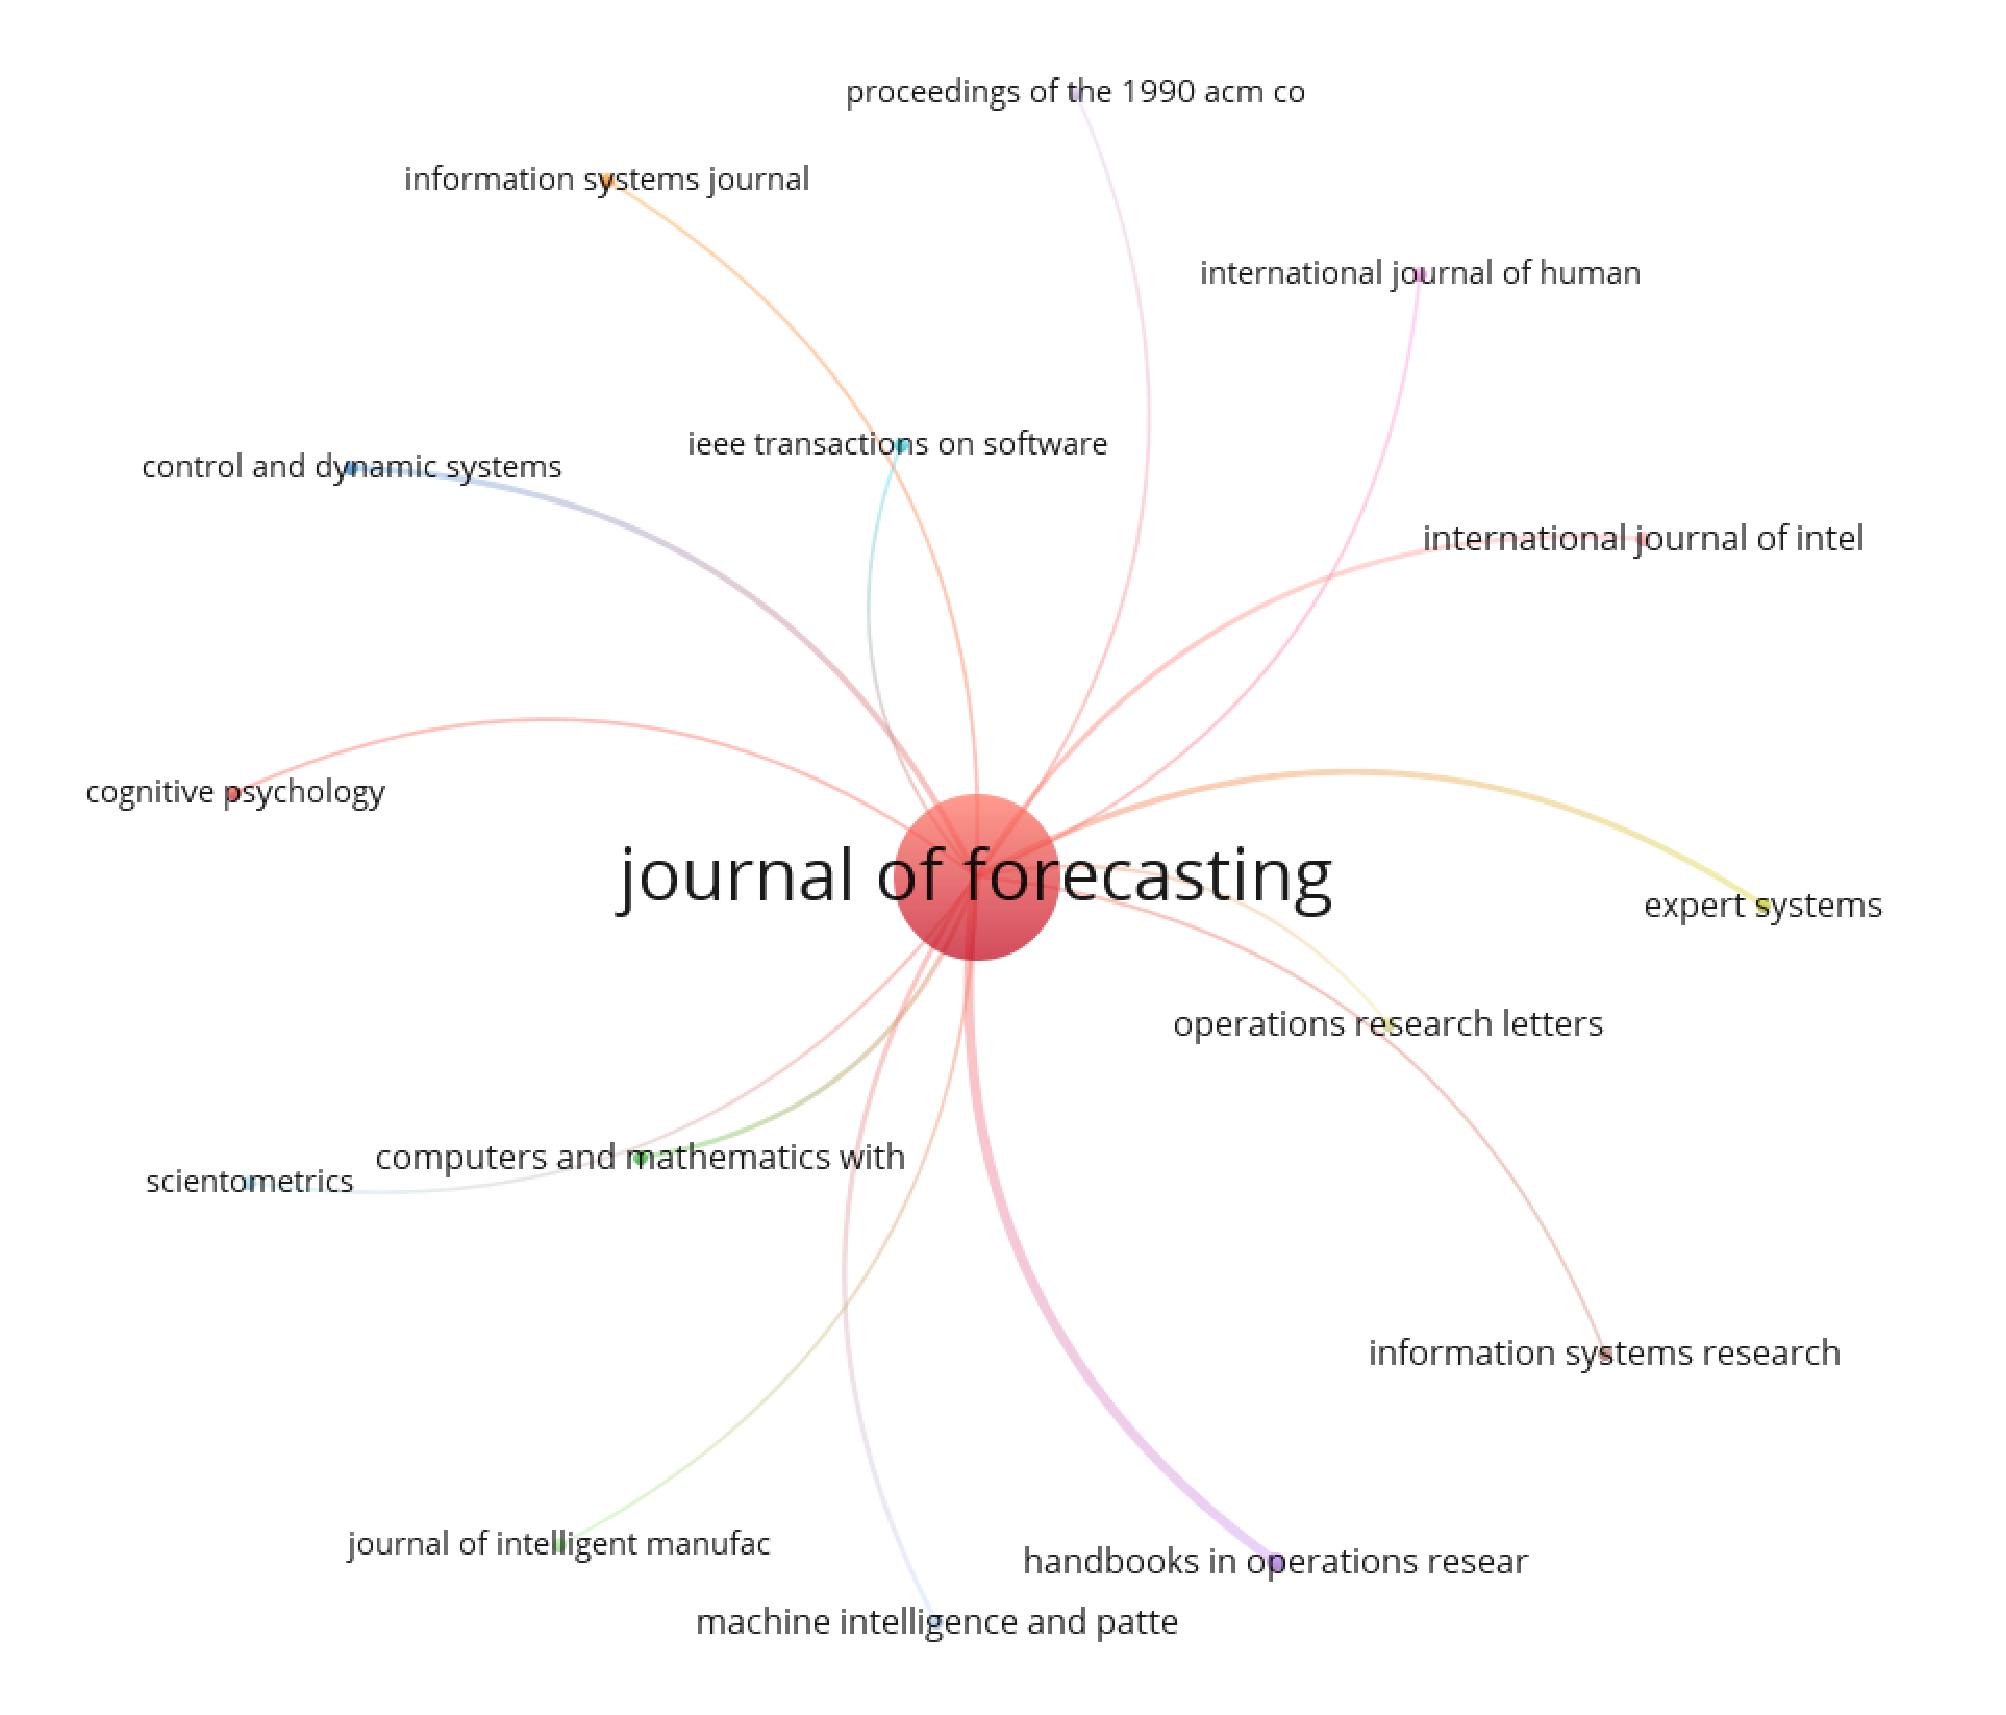
\includegraphics[scale=0.4]{fig.20.eps}
\caption{JF Journal citation network in Computer Science from 1982 to 1994}
\end{figure}

\begin{figure}[htbp]
\centering
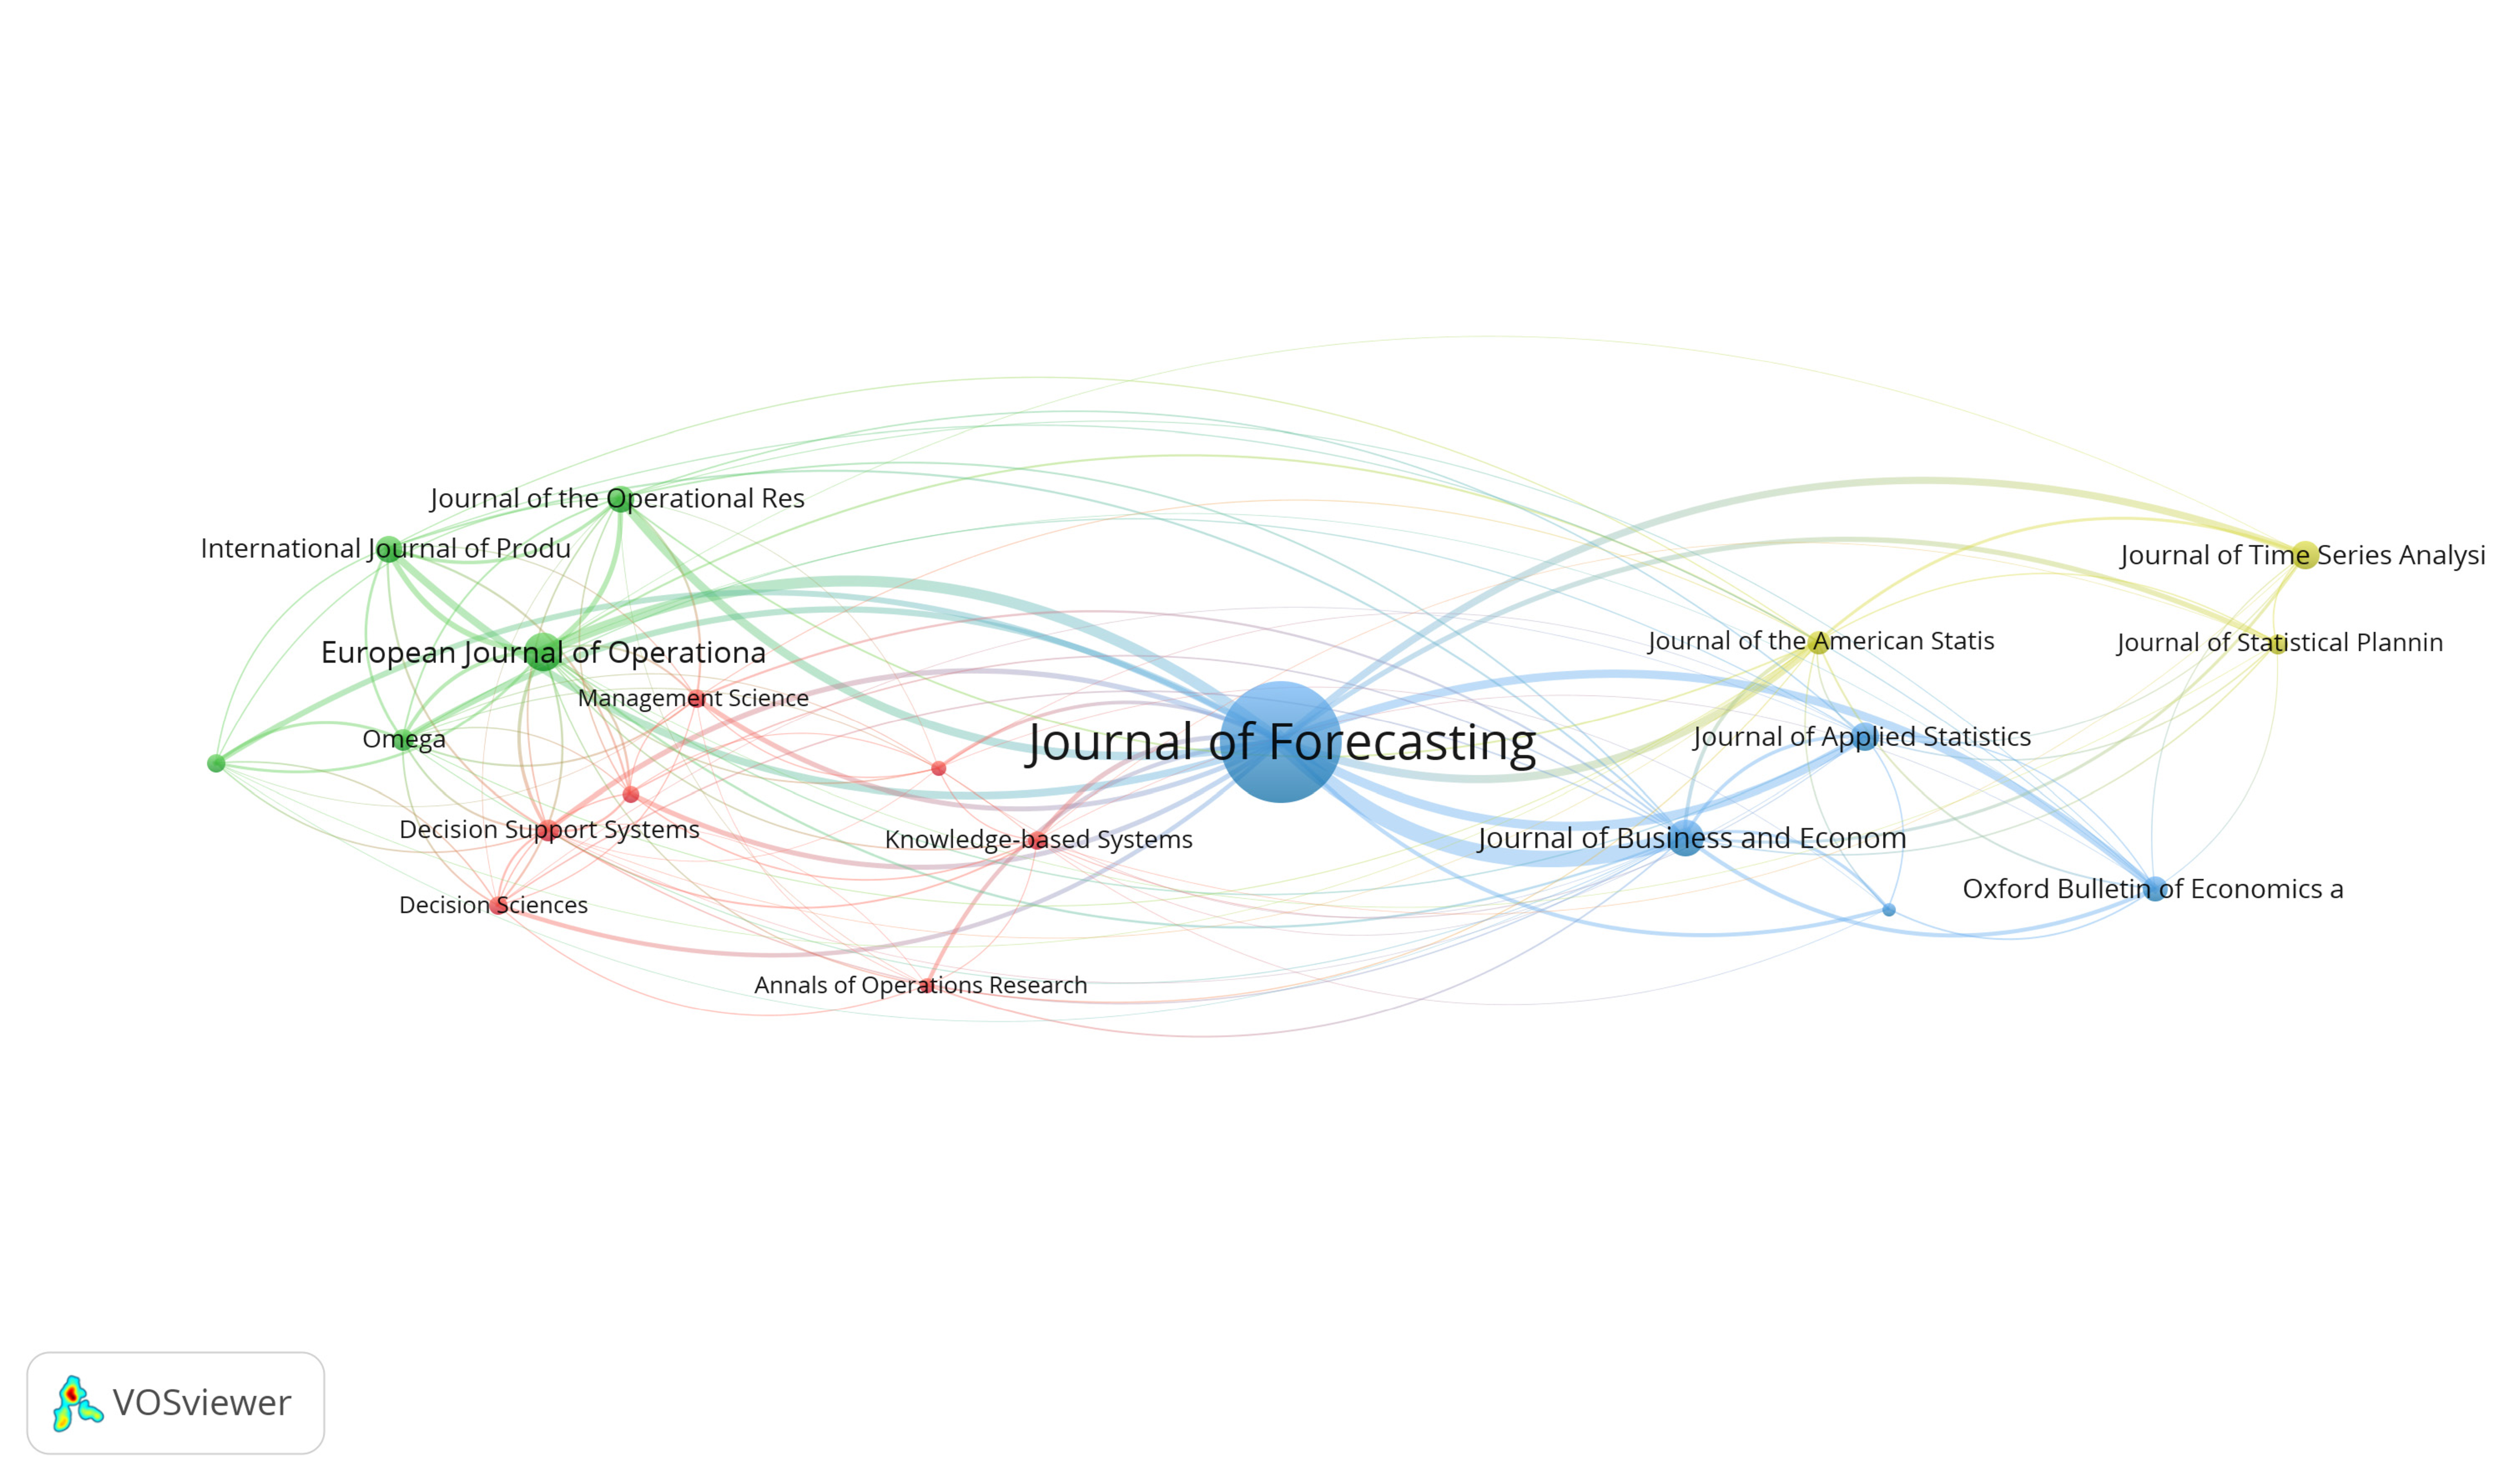
\includegraphics[scale=0.3]{fig.21.eps}
\caption{JF Journal citation network in Computer Science from 1995 to 2009}
\end{figure}

\begin{figure}[htbp]
\centering

\includegraphics[scale=0.3]{fig.22.eps}
\caption{JF Journal citation network in Computer Science from 2008 to 2019  }
\end{figure}

\begin{landscape}
\begin{table}[!htbp]
    \centering
    \caption{The information about the journal citation networks in Computer Science based on the JF citing papers}
    \setlength{\tabcolsep}{0.3mm}{
    \begin{tabular}{p{1.5cm}<{\centering} p{6cm}<{\centering} p{1.5cm}<{\centering}|p{1.5cm}<{\centering} p{6cm}<{\centering} p{1.5cm}<{\centering}|p{1.5cm}<{\centering} p{6cm}<{\centering} p{1.5cm}<{\centering}}
    \hline
        \hline
        \multicolumn{3}{c|}{1985-1996} & \multicolumn{3}{c|}{1997-2008} & \multicolumn{3}{c}{2009-2019}\\
    \hline
    \multicolumn{9}{c}{Limiting condition}\\
    \hline
        \multicolumn{3}{c|}{Number>=1 Citation>=10} & \multicolumn{3}{c|}{Number>=5 Citation>=200} & \multicolumn{3}{c}{Number>=40 Citation>=200}\\
    \hline
    \multicolumn{9}{c}{Parameters}\\
    \hline
    Clusters & Local links & Link strength & Clusters & Local links & Link strength & Clusters & Local links & Link strength\\
    9 & 18 & 173 & 8    & 66 & 1025 & 7 & 168 & 6146\\
        \hline
        \hline
   R & Journal & Links & R & Journal & Links & R & Journal & Links\\
1 & Handbooks in Operations Research and Management Science & 8 & 1 & Computational Statistics and Data Analysis & 60 & 1 & Expert Systems with Applications & 154\\
2 & Control and Dynamic Systems & 3 & 2 & Lecture Notes in Computer Science & 49 & 2 & Computational Statistics and Data Analysis & 85\\
3 & Expert Systems & 3 & 3 & Computers and Operations Research & 41 & 3 & Lecture Notes in Computer Science & 80\\
4 & Computers and Mathematics with Applications & 2 & 4 & European Journal of Operational Research & 31 & 4 & Neurocomputing & 66\\
5 & International Journal of Intelligent Systems & 2 & 5 & Environmental Modelling and Software & 24 & 5 & European Journal of Operational Research & 63\\
6 & Machine Intelligence and Pattern Recognition & 2 & 6 & IEEE Transactions on Neural Networks & 23 & 6 & Proceedings of The International Joint Conference on Neural Networks & 56\\
7 & Cognitive Psychology & 1 & 7 & Neurocomputing & 22 & 7 & Computational Economics & 55\\
8 & IEEE Transactions on Software Engineering & 1 & 8 & Decision Support Systems & 20 & 8 & Applied Soft Computing Journal & 53\\
9 & Information Systems Journal & 1 & 9 & Computational Economics & 19 & 9 & Knowledge-Based Systems & 50\\
10 & Information Systems Research & 1 & 10 & IEEE International Conference on Neural Networks & 17 & 10 & Mathematics and Computers in Simulation & 47\\
  \hline
  \hline
    \end{tabular}}
\end{table}
\end{landscape}

\noindent 3.2.2.2. Journal citation network in Economics, Econometrics
and Finance

The citation networks based on the IJF papers and their citing papers
belonging to Economics, Econometrics and Finance are depicted in Fig.
23-25. The citation network structure of this subject area is kind of
stable because four citing journals appear in the list of top ten most
citing journals in three periods, which are Journal of Business and
Economic Statistics, Applied Economics, Journal of Econometrics, and
Journal of Applied Econometrics. Moreover, except for the four journals
mentioned above, another three journals also appears in both period 2
and 3, which are Oxford Bulletin of Economics and Statistics, Economic
Modelling, and International Journal of Production Economics. There are
seven of the ten journals both appear in period 2 and 3, and it means
the most royal audiences of this subject area are very stable during the
past 25 years. Besides, the network structures of Fig. 24 and Fig. 25
are very similar where the most journals are located in the left side of
the figures and leaving one or two journals in the right side.
International Journal of Production Economics is a journal that locates
in the right side of the Fig. 24 and 25, which indicates it is a
prolific citing journal of JF but its content similarity with JF is much
weaker than that of journals in the left side.

\begin{figure}[htbp]
\centering
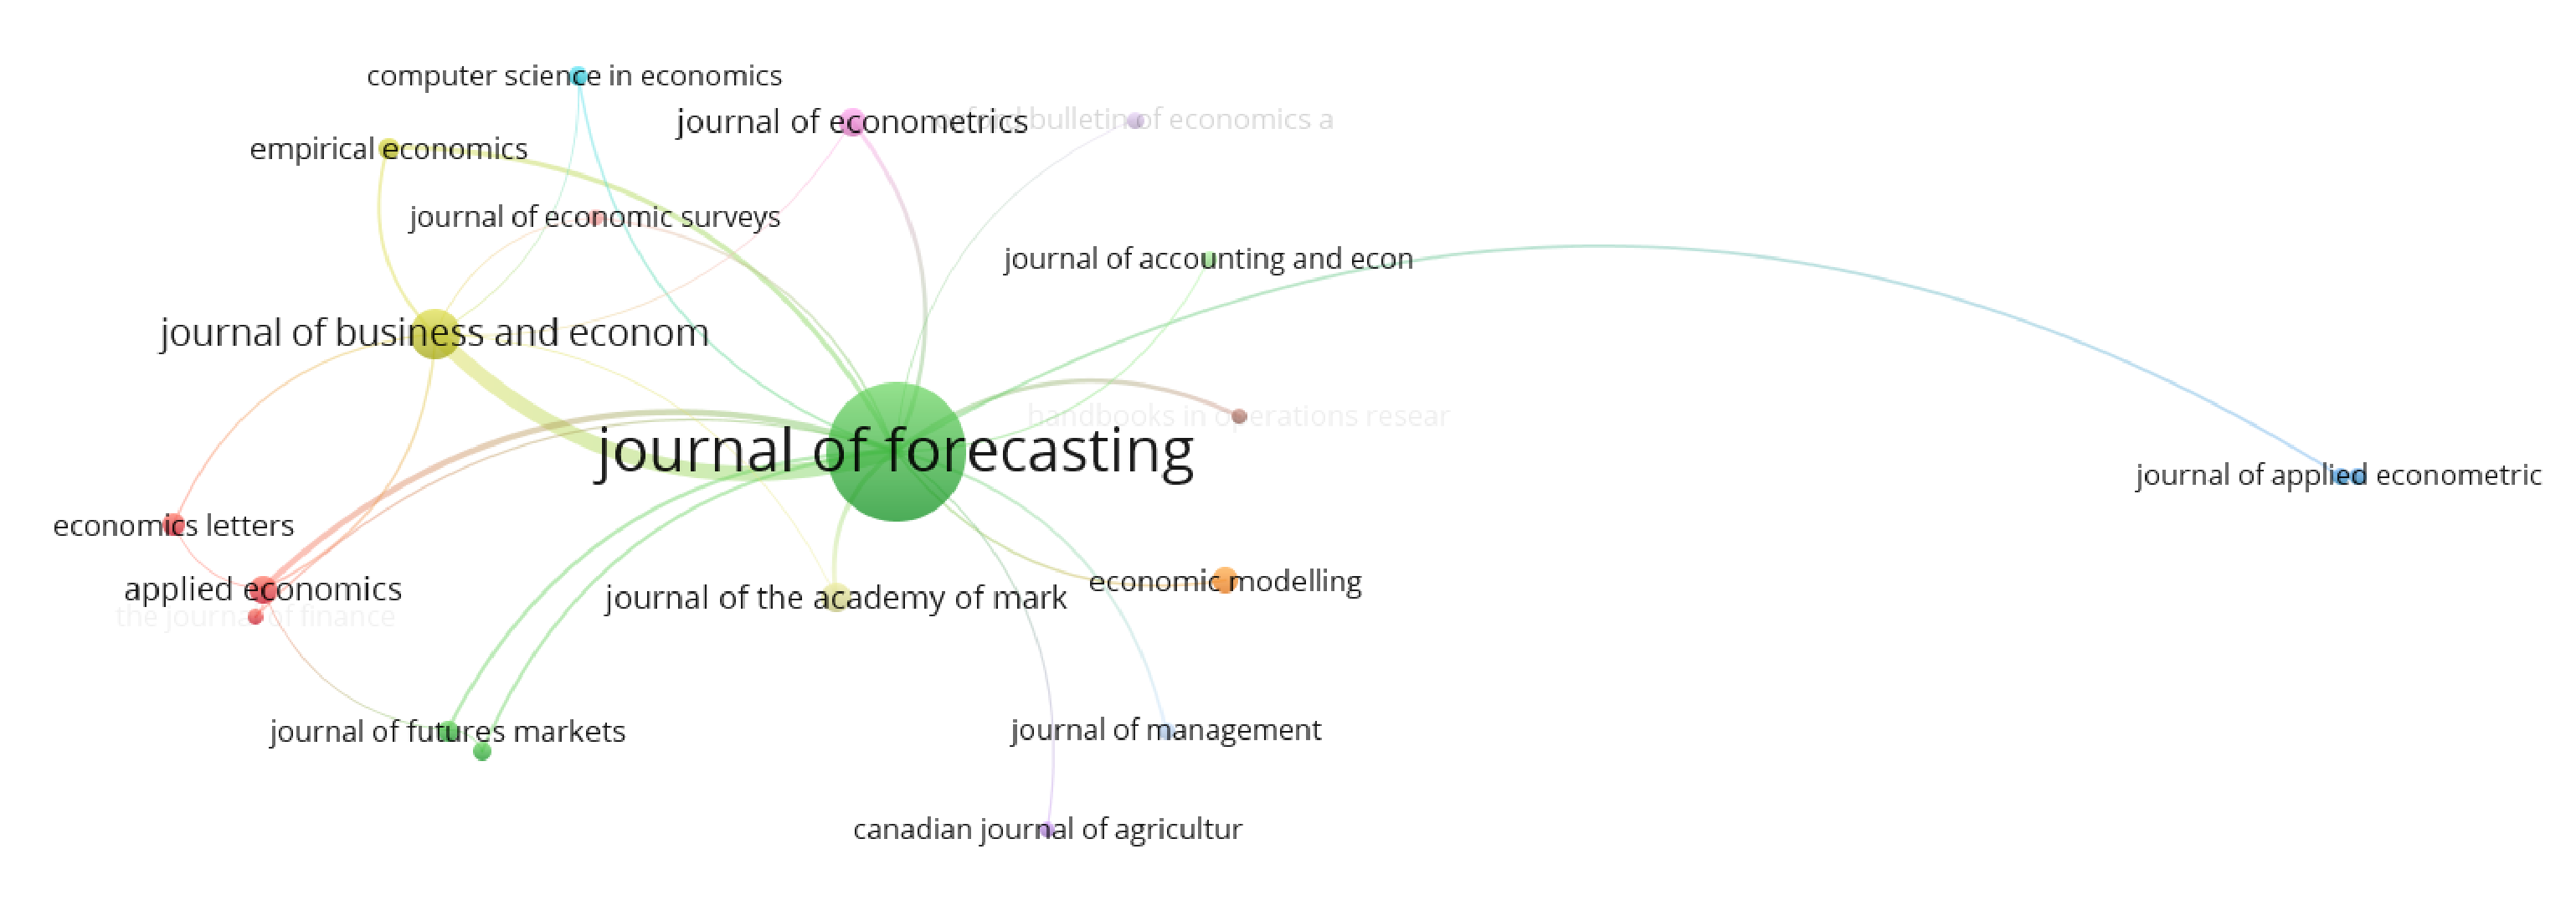
\includegraphics[scale=0.3]{fig.23.eps}
\caption{JF Journal citation network in Economics, Econometrics and Finance from 1982 to 1994}
\end{figure}

\begin{figure}[htbp]
\centering
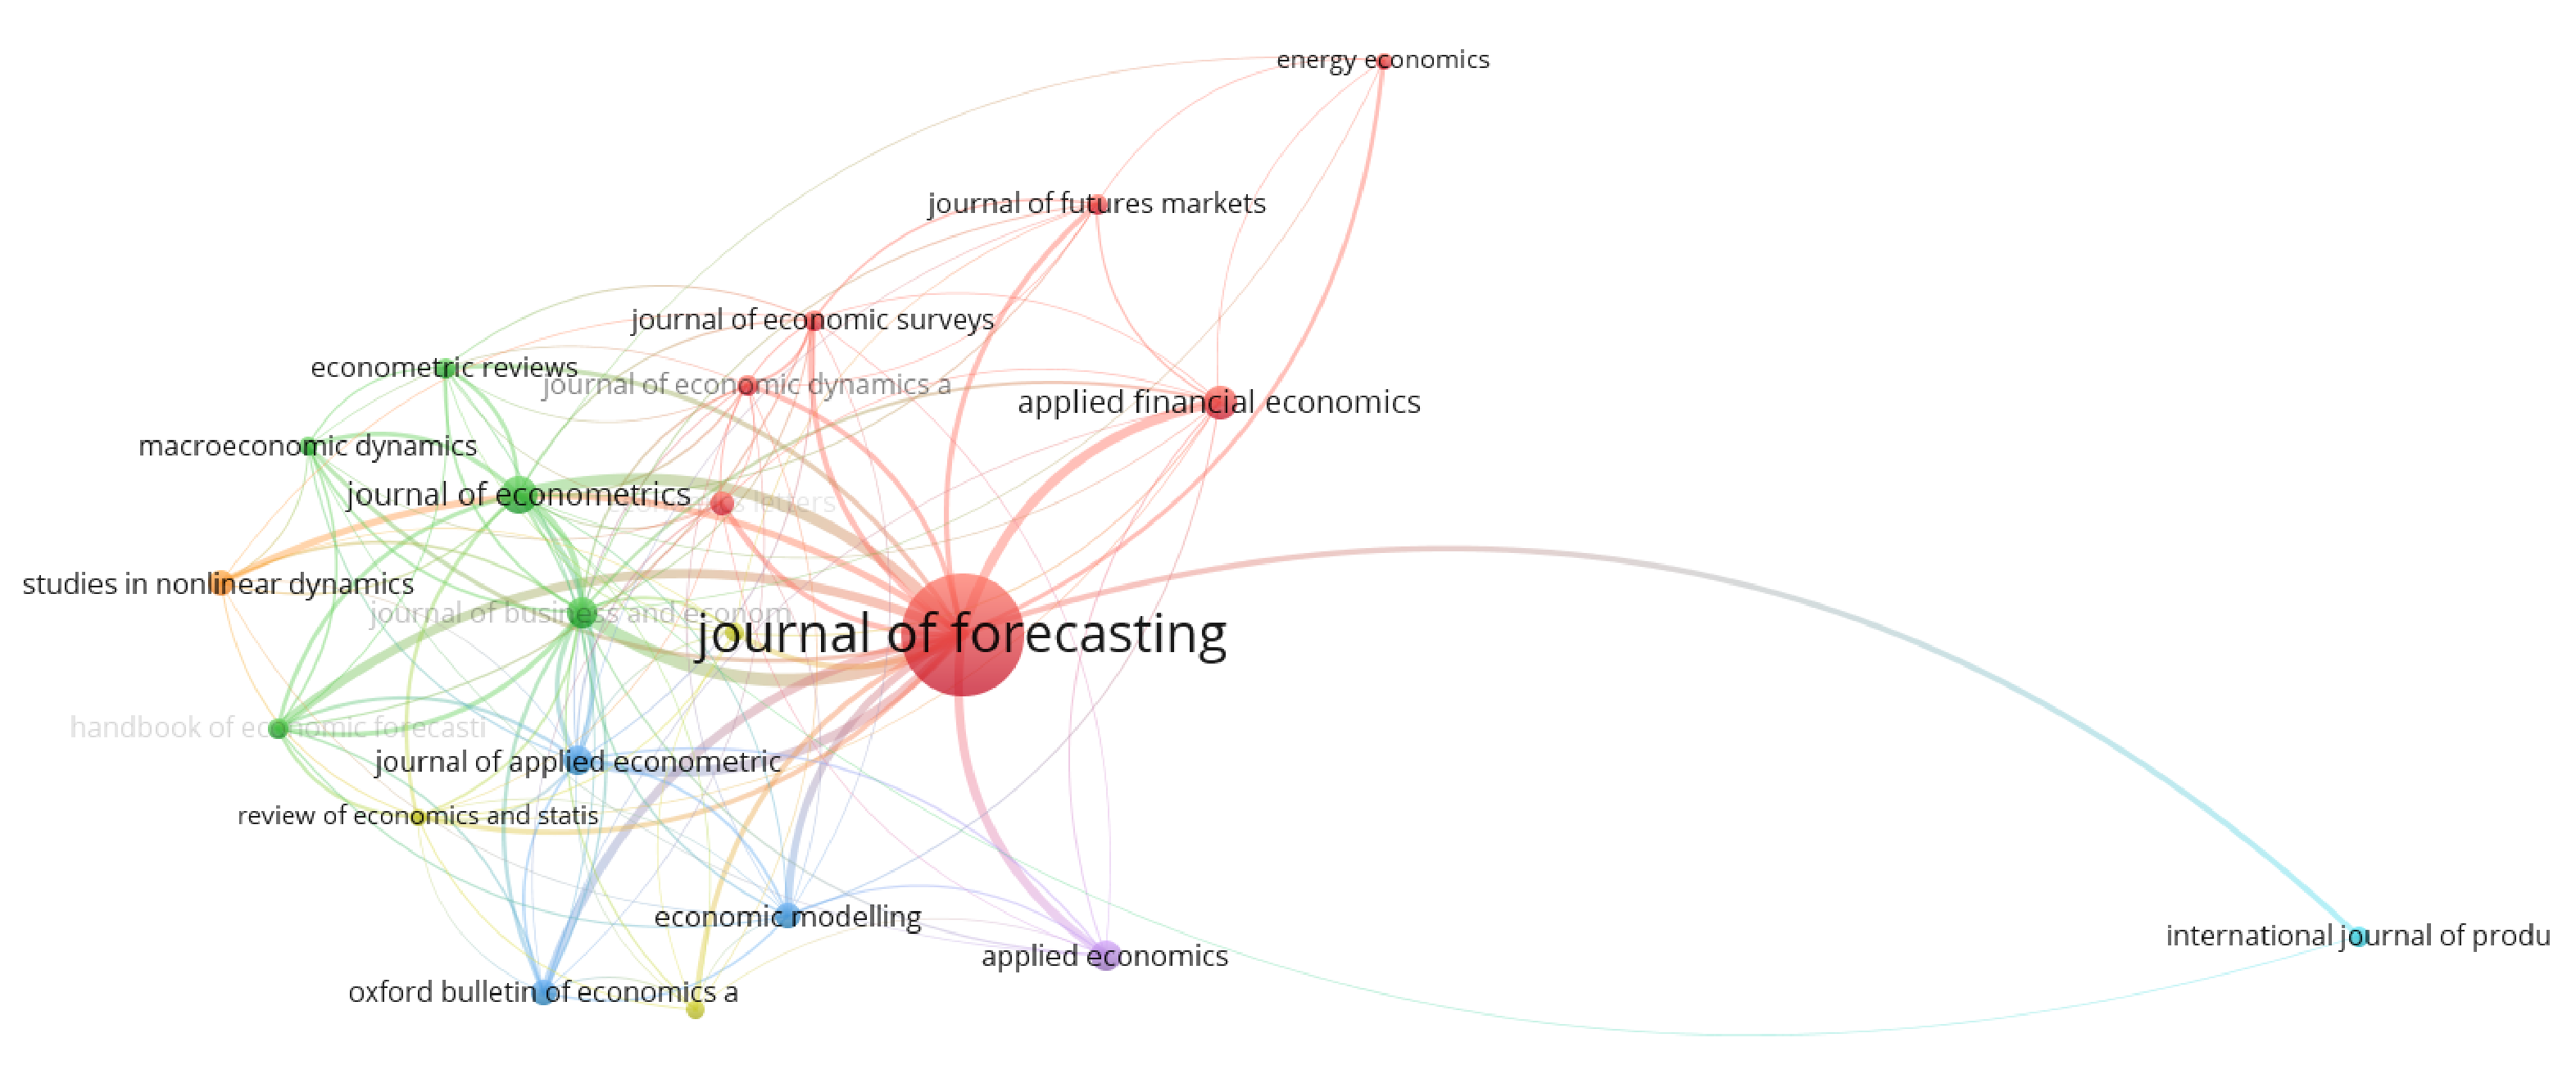
\includegraphics[scale=0.3]{fig.24.eps}
\caption{JF Journal citation network in Economics, Econometrics and Finance from 1995 to 2007}
\end{figure}

\begin{figure}[htbp]
\centering
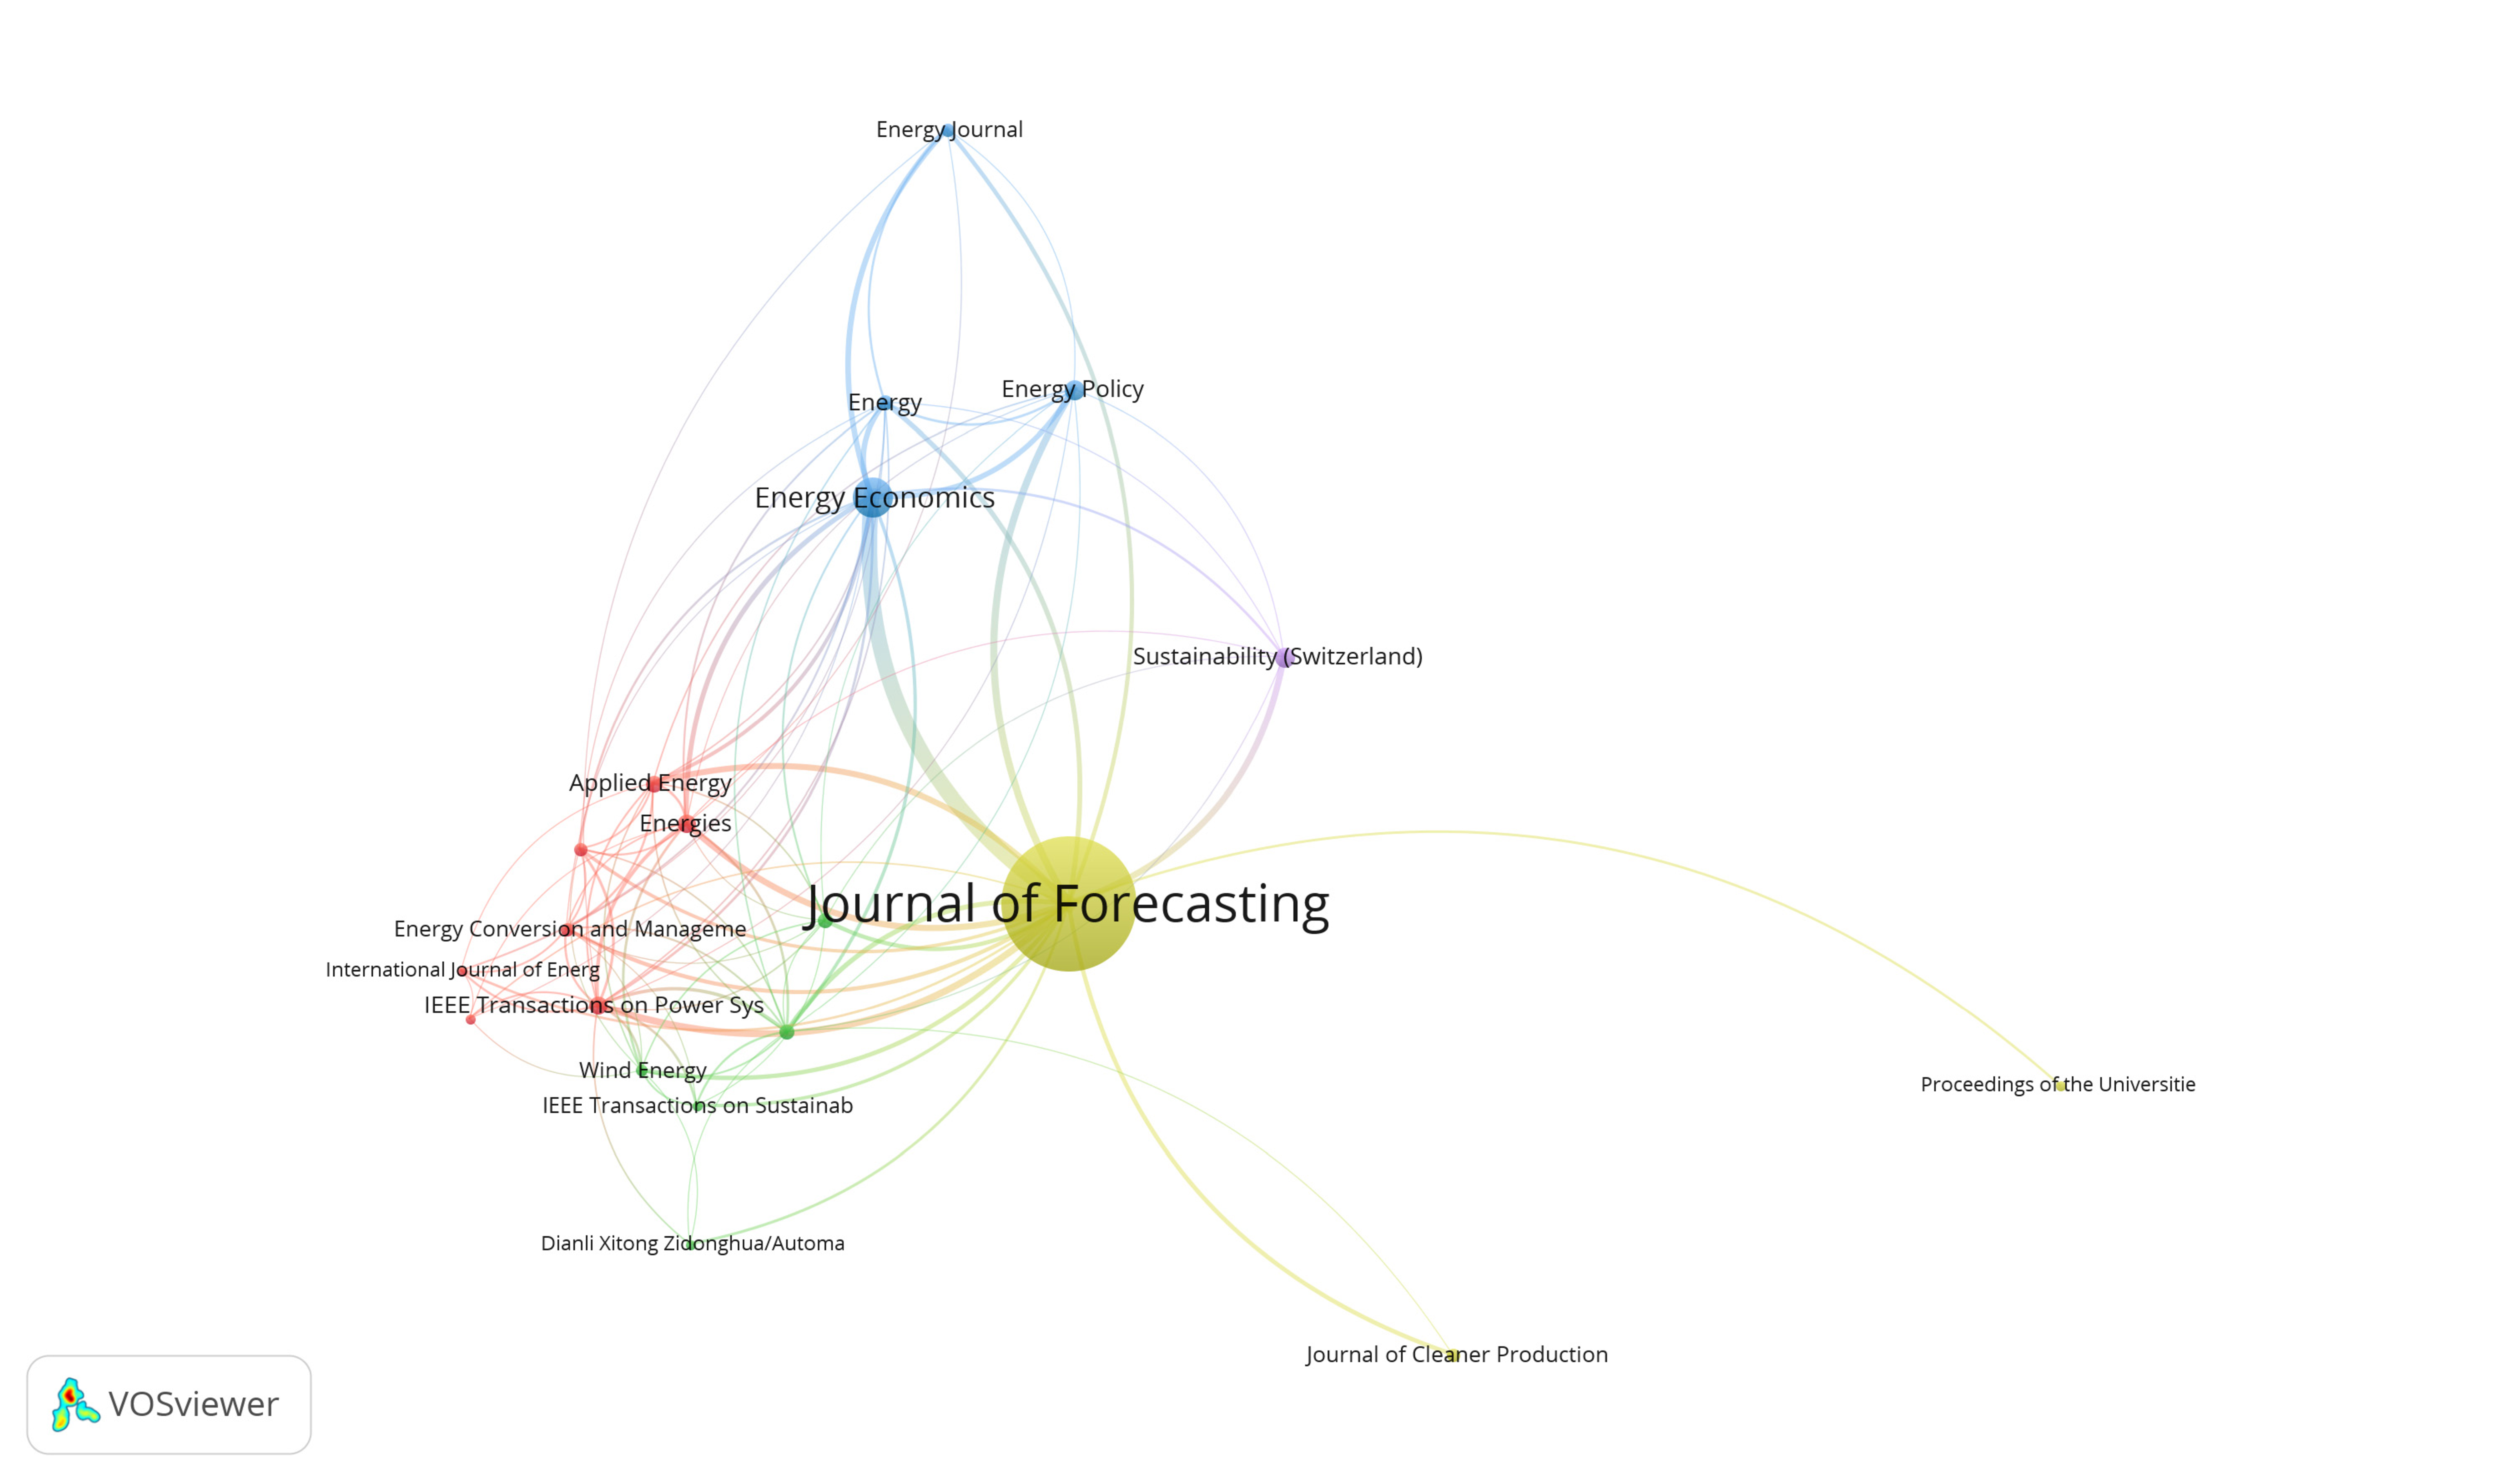
\includegraphics[scale=0.3]{fig.25.eps}
\caption{JF Journal citation network in Economics, Econometrics and Finance from 2008 to 2019}
\end{figure}

\begin{landscape}
\begin{table}[!htbp]
    \centering
    \caption{The information about the journal citation networks in Economics, Econometrics and Finance based on the JF citing papers}
    \setlength{\tabcolsep}{0.3mm}{
    \begin{tabular}{p{1.5cm}<{\centering} p{6cm}<{\centering} p{1.5cm}<{\centering}|p{1.5cm}<{\centering} p{6cm}<{\centering} p{1.5cm}<{\centering}|p{1.5cm}<{\centering} p{6cm}<{\centering} p{1.5cm}<{\centering}}
    \hline
        \hline
        \multicolumn{3}{c|}{1985-1996} & \multicolumn{3}{c|}{1997-2008} & \multicolumn{3}{c}{2009-2019}\\
    \hline
    \multicolumn{9}{c}{Limiting condition}\\
    \hline
        \multicolumn{3}{c|}{Number>=1 Citation>=10} & \multicolumn{3}{c|}{Number>=5 Citation>=200} & \multicolumn{3}{c}{Number>=40 Citation>=200}\\
    \hline
    \multicolumn{9}{c}{Parameters}\\
    \hline
    Clusters & Local links & Link strength & Clusters & Local links & Link strength & Clusters & Local links & Link strength\\
    9 & 18 & 173 & 8    & 66 & 1025 & 7 & 168 & 6146\\
        \hline
        \hline
   R & Journal & Links & R & Journal & Links & R & Journal & Links\\
1 & Journal of Business and Economic Statistics & 98 & 1 & Journal of Business and Economic Statistics & 124 & 1 & Economic Modelling & 199\\
2 & Applied Economics & 16 & 2 & Journal of Econometrics & 90 & 2 & Energy Economics & 165\\
3 & Empirical Economics & 10 & 3 & Journal of Applied Econometrics & 70 & 3 & Journal of Econometrics & 154\\
4 & Journal of the Academy of Marketing Science & 10 & 4 & Applied Financial Economics & 66 & 4 & Applied Economics & 149\\
5 & Handbooks in Operations Research and Management Science & 8 & 5 & Handbook of Economic Forecasting & 63 & 5 & Journal of Business and Economic Statistics & 104\\
6 & Journal of Econometrics & 8 & 6 & Applied Economics & 57 & 6 & Journal of Applied Econometrics & 101\\
7 & Journal of Futures Markets & 6 & 7 & Oxford Bulletin of Economics and Statistics & 56 & 7 & International Journal of Production Economics & 90\\
8 & American Journal of Agricultural Economics & 5 & 8 & Economic Modelling & 41 & 8 & International Review of Economics and Finance & 75\\
9 & Journal of Applied Econometrics & 4 & 9 & Studies in Nonlinear Dynamics And Econometrics & 33 & 9 & Quantitative Finance & 72\\
10 & Journal of Management & 4 & 10 & International Journal of Production Economics & 24 & 10 & Oxford Bulletin of Economics and Statistics & 62\\
  \hline
  \hline
    \end{tabular}}
\end{table}
\end{landscape}

\noindent 3.2.2.3. Journal citation network in Engineering

As shown in Fig. 26-28, the journal citation relationships between JF
papers and their citing papers in Engineering are described based on the
citation networks. In Engineering, the total link strength in period 3
is 632, which is much weaker than the above two subject areas.
Therefore, the journal citation strength between JF and other related
journals is weak in Engineering. In table 18, one citing journal appears
in the period 1 and 2, and another citing journal appears in the period
1 and 3. Further, three citing journals in the period 2 also appears in
the period 3. This journal overlapping phenomenon indicates that in
Engineering, the citing journals keep a limited continuity in knowledge
diffusion starting from JF. Expert Systems with Applications first
appears and becomes the top one citing journal in the period 3,
moreover, the number of citation links it possesses is much more than
that of International Journal of Production Economics (i.e., the second
most citing journals in the period 3). In addition, similar to the
situation of the knowledge diffusion from IJF in Engineering, there is a
new cluster containing some energy-related journals emerging in the
period 3, as shown in the right side of the Fig. 28. Therefore, it
proves that JF attracts some energy-related journals in the past ten
years, which is the same as IJF.

\begin{figure}[htbp]
\centering
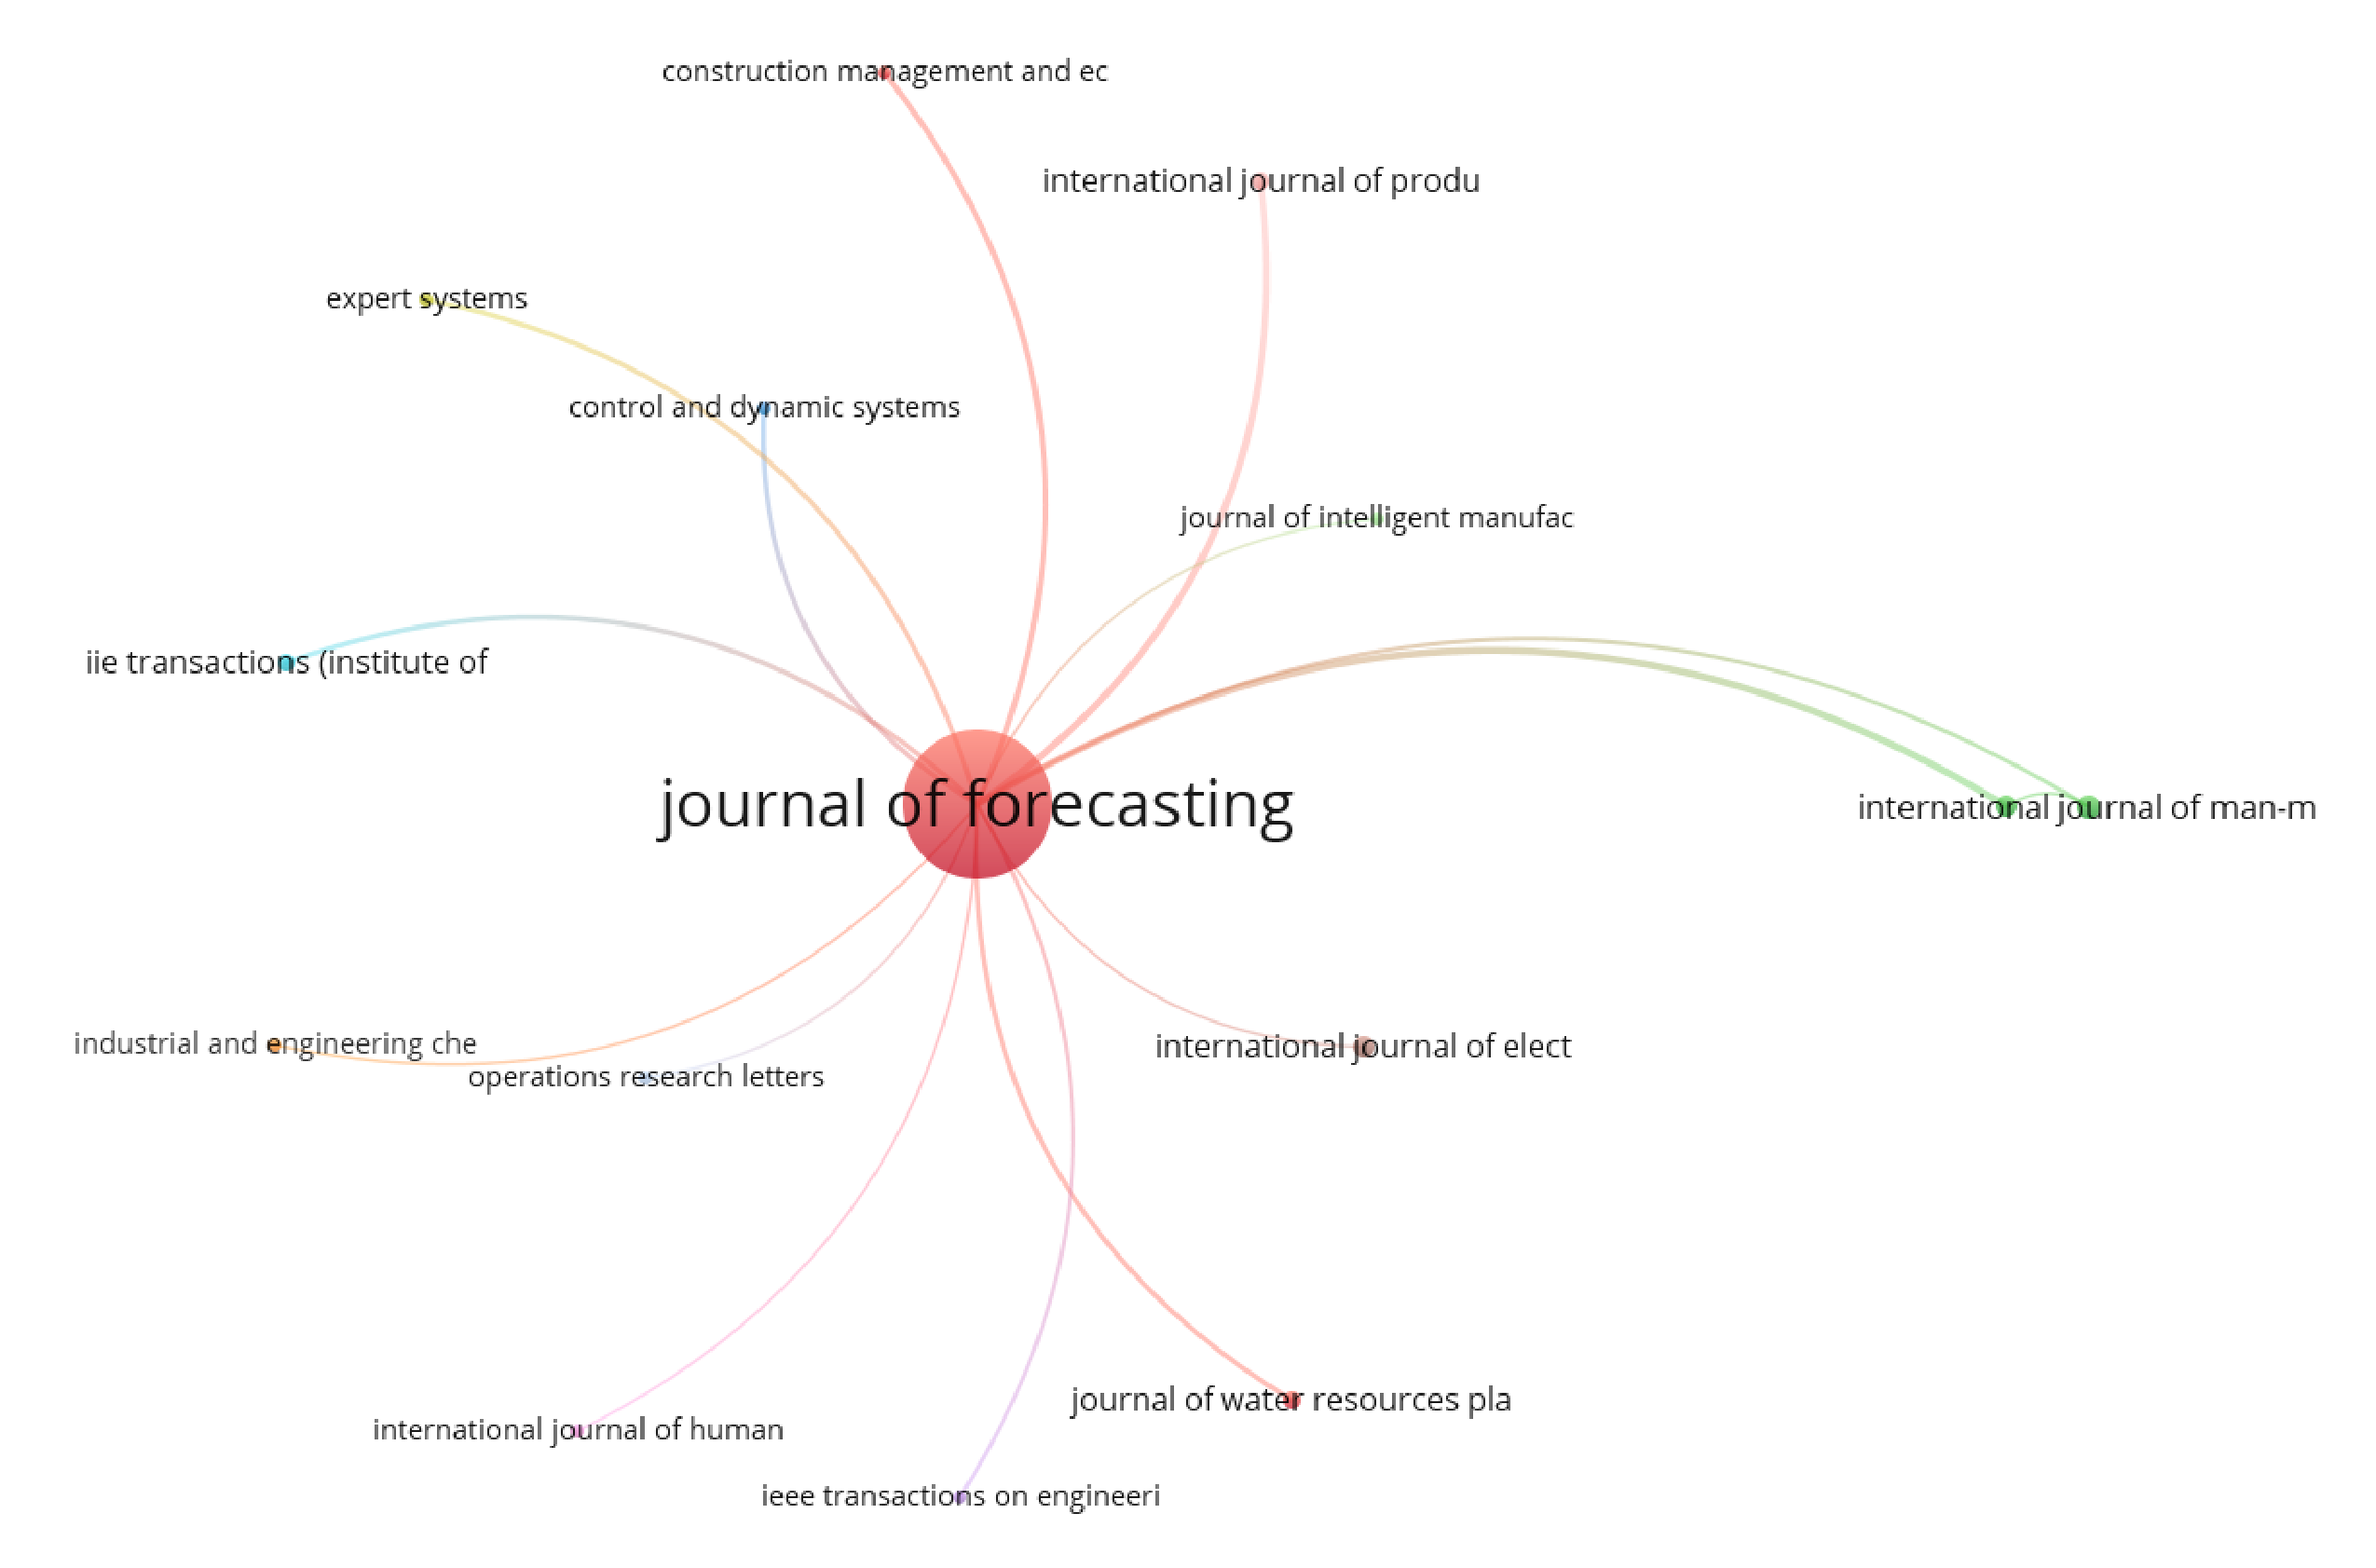
\includegraphics[scale=0.3]{fig.26.eps}
\caption{JF Journal citation network in Engineering from 1982 to 1994}
\end{figure}

\begin{figure}[htbp]
\centering
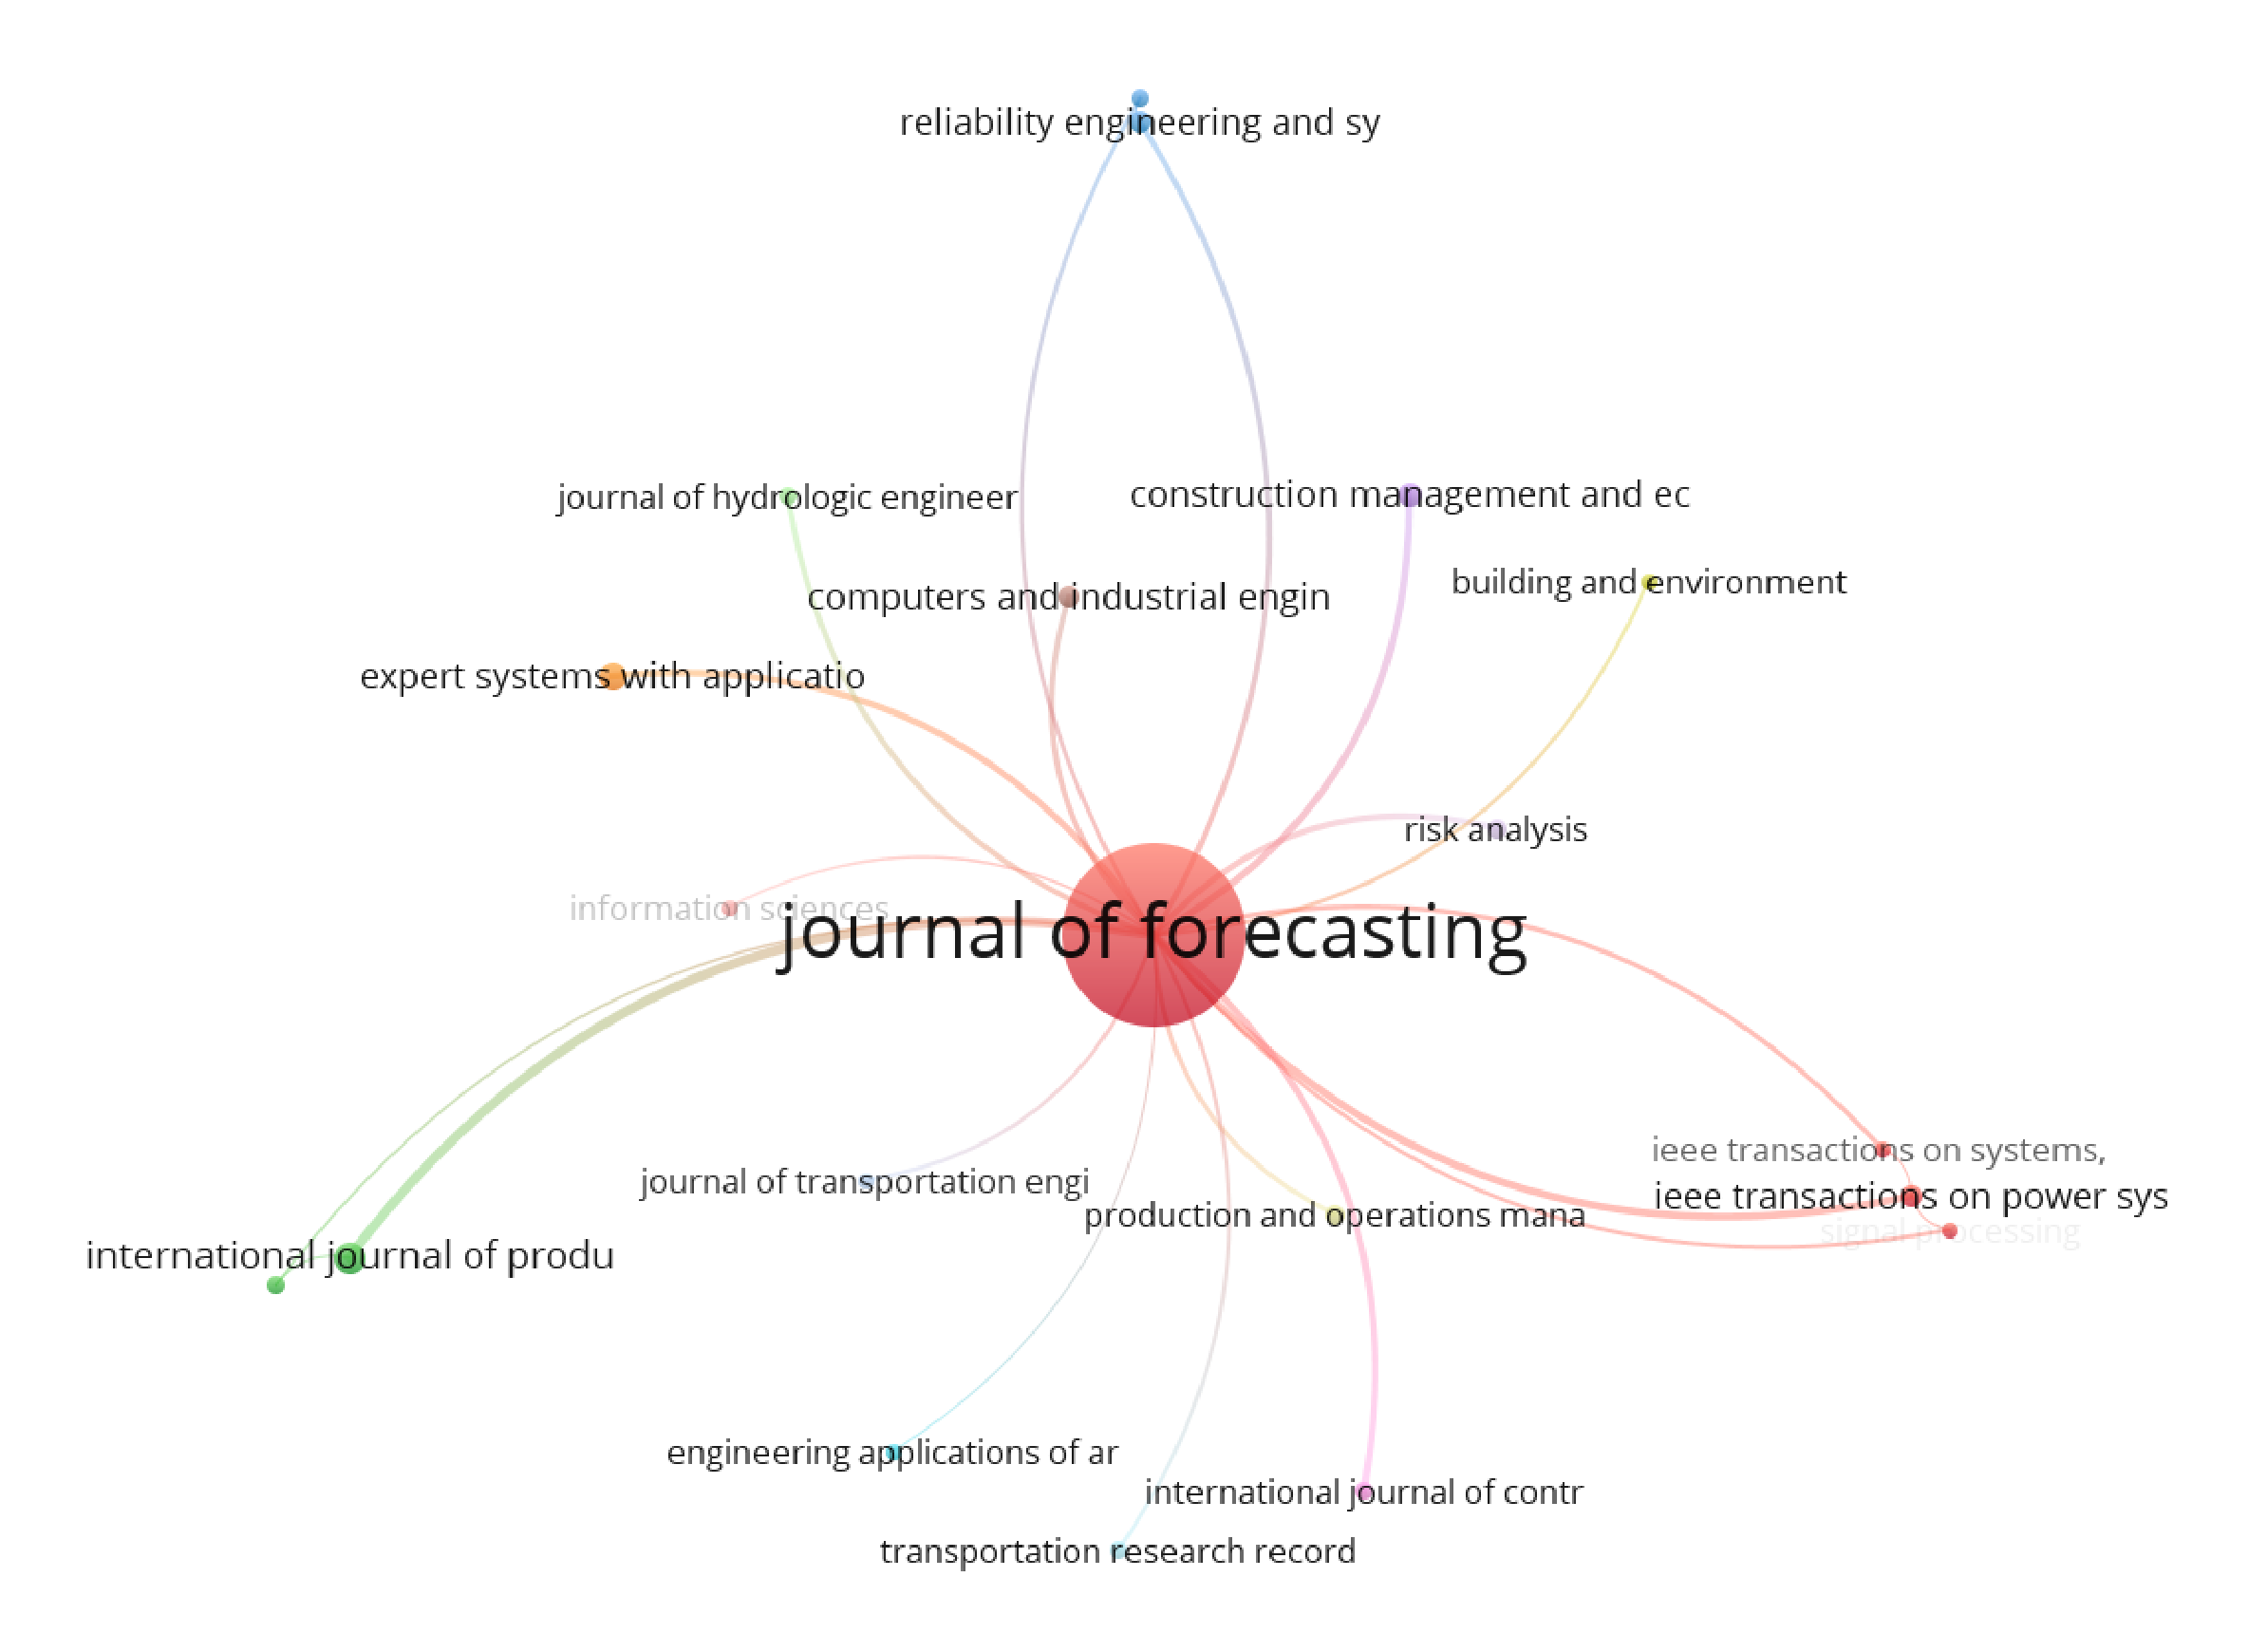
\includegraphics[scale=0.3]{fig.27.eps}
\caption{JF Journal citation network in Engineering from 1995 to 2007}
\end{figure}

\begin{figure}[htbp]
\centering
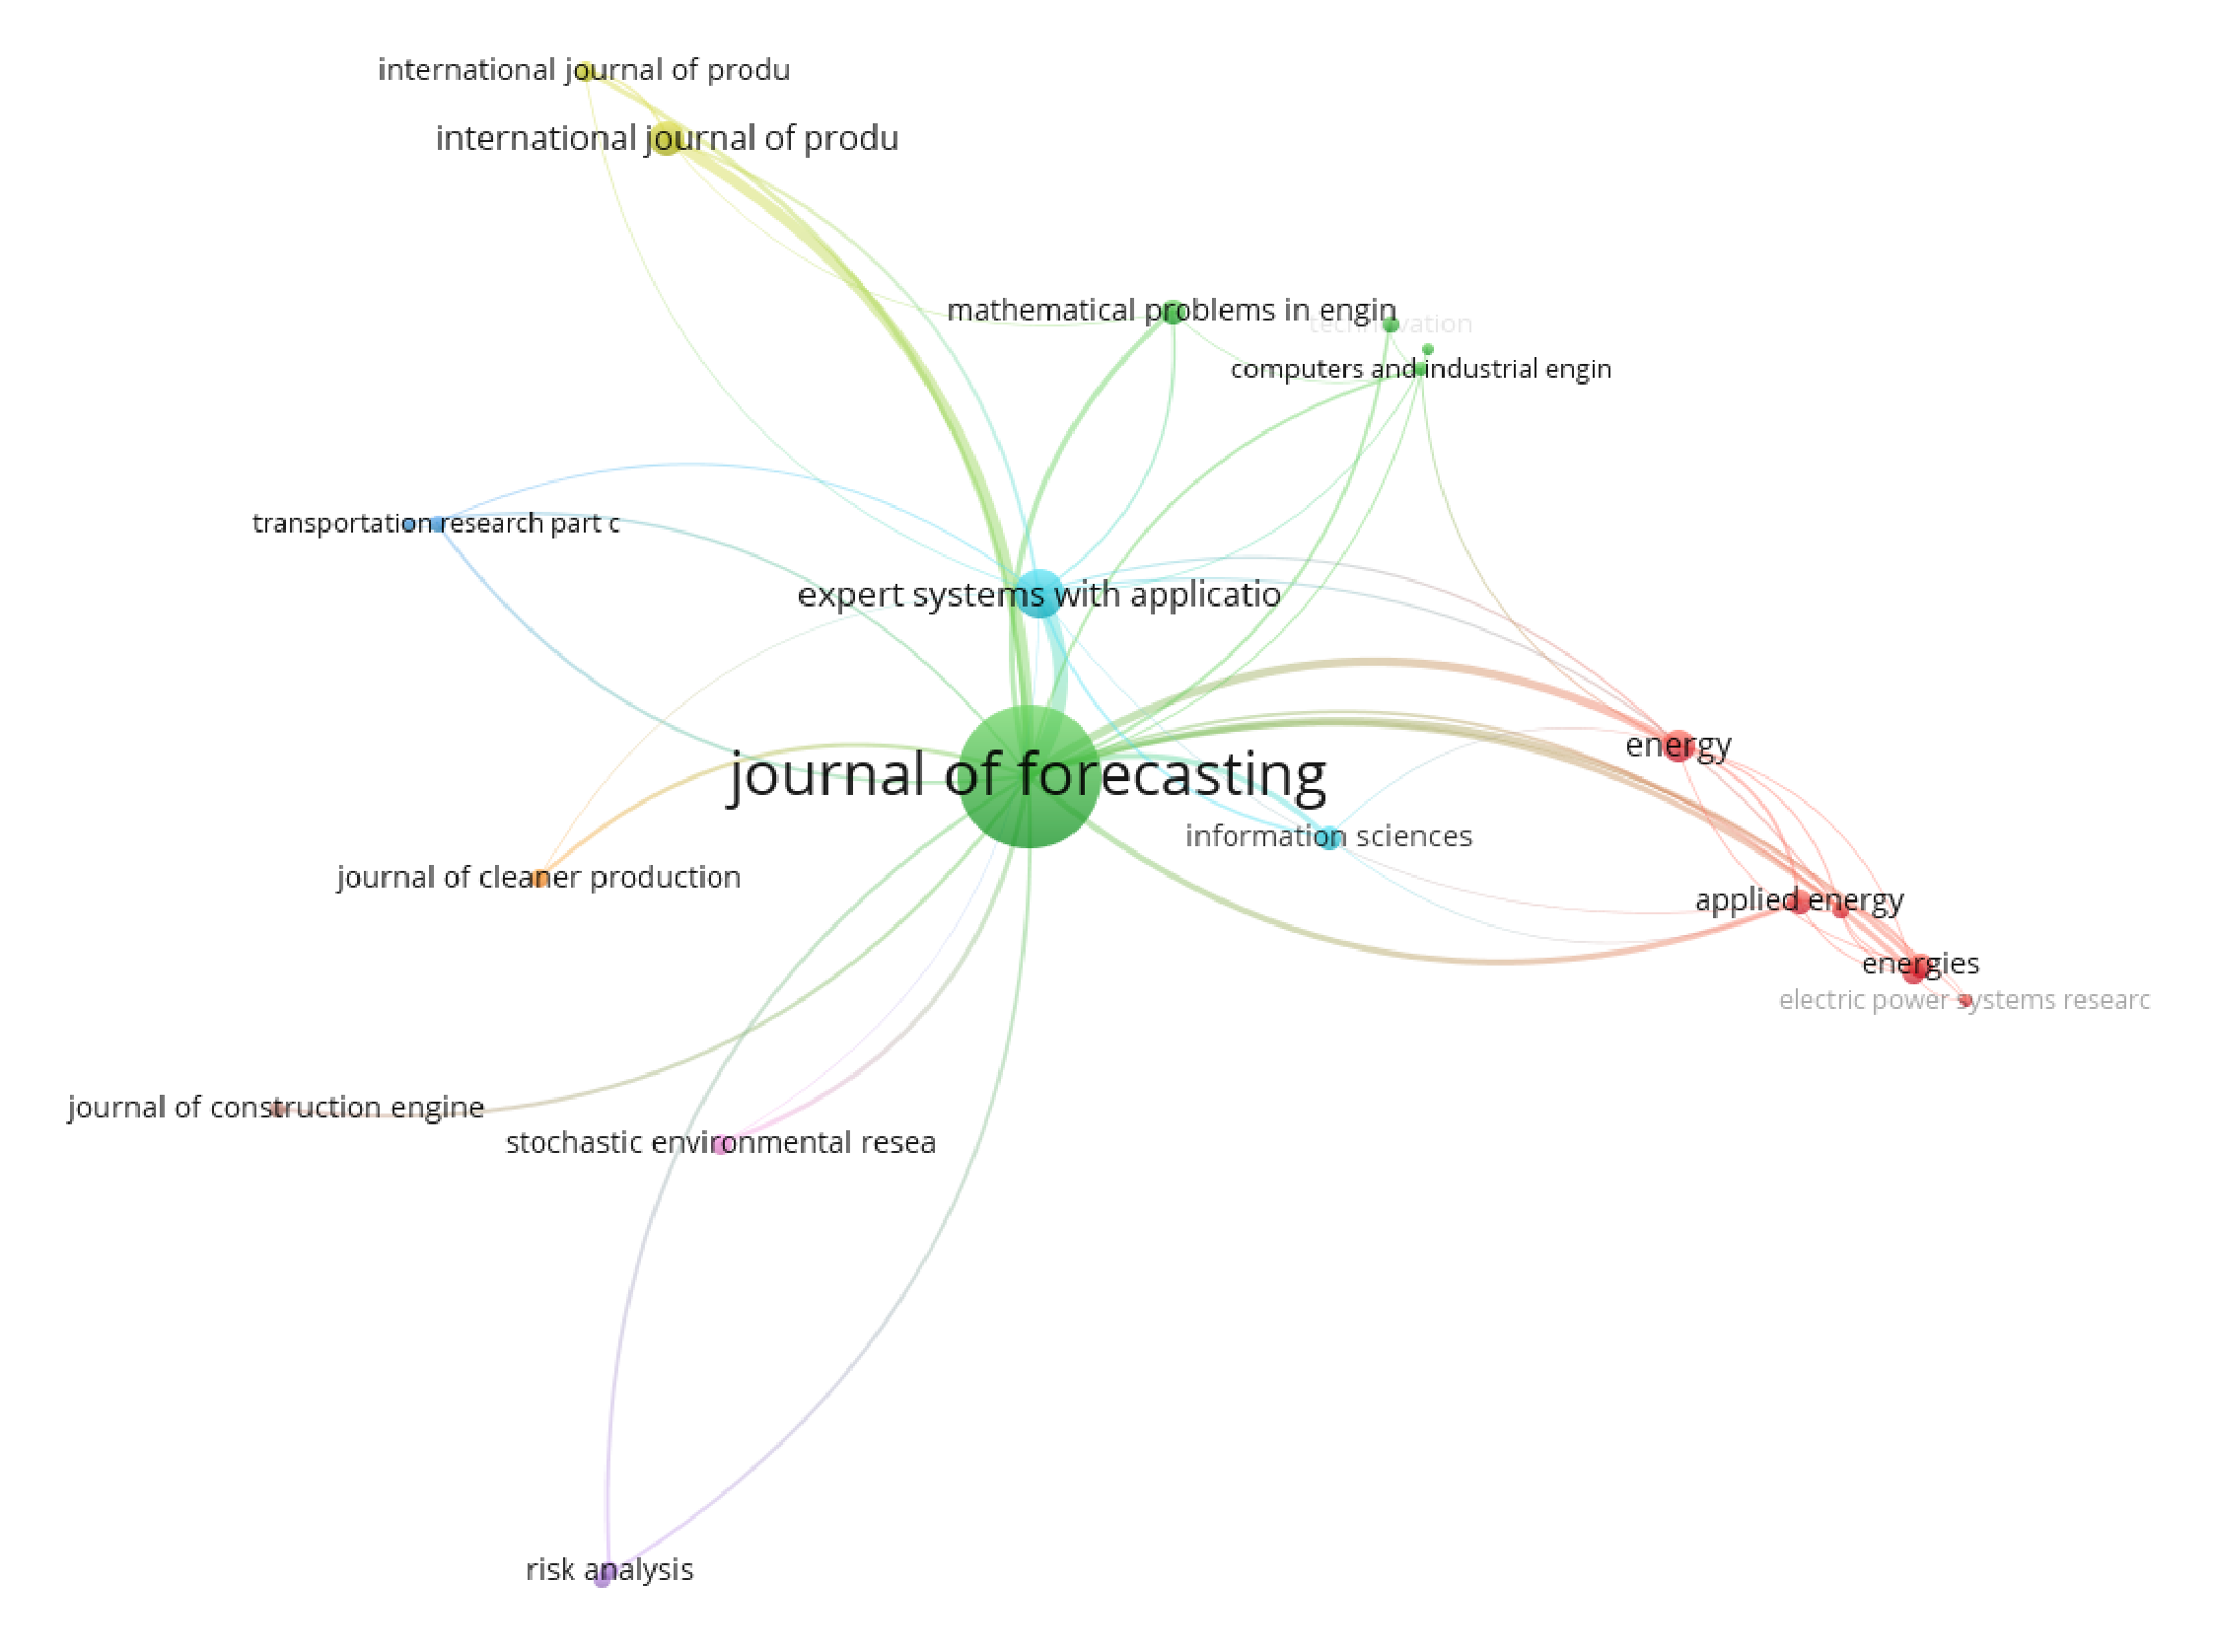
\includegraphics[scale=0.3]{fig.28.eps}
\caption{JF Journal citation network in Engineering from 2008 to 2019}
\end{figure}

\begin{landscape}
\begin{table}[!htbp]
    \centering
    \caption{The information about the journal citation networks in Engineering based on the JF citing papers}
    \setlength{\tabcolsep}{0.3mm}{
    \begin{tabular}{p{1.5cm}<{\centering} p{6cm}<{\centering} p{1.5cm}<{\centering}|p{1.5cm}<{\centering} p{6cm}<{\centering} p{1.5cm}<{\centering}|p{1.5cm}<{\centering} p{6cm}<{\centering} p{1.5cm}<{\centering}}
    \hline
        \hline
        \multicolumn{3}{c|}{1985-1996} & \multicolumn{3}{c|}{1997-2008} & \multicolumn{3}{c}{2009-2019}\\
    \hline
    \multicolumn{9}{c}{Limiting condition}\\
    \hline
        \multicolumn{3}{c|}{Number>=1 Citation>=10} & \multicolumn{3}{c|}{Number>=5 Citation>=200} & \multicolumn{3}{c}{Number>=40 Citation>=200}\\
    \hline
    \multicolumn{9}{c}{Parameters}\\
    \hline
    Clusters & Local links & Link strength & Clusters & Local links & Link strength & Clusters & Local links & Link strength\\
    9 & 18 & 173 & 8    & 66 & 1025 & 7 & 168 & 6146\\
        \hline
        \hline
   R & Journal & Links & R & Journal & Links & R & Journal & Links\\
1 & IEEE Transactions on Systems, Man and Cybernetics & 6 & 1 & International Journal of Production Economics & 24 & 1 & Expert Systems with Applications & 154\\
2 & International Journal of Production Research & 6 & 2 & IEEE Transactions on Power Systems & 14 & 2 & International Journal of Production Economics & 90\\
3 & Construction Management and Economics & 4 & 3 & Construction Management and Economics & 13 & 3 & Energy & 54\\
4 & Control and Dynamic Systems & 3 & 4 & Expert Systems with Applications & 11 & 4 & Applied Energy & 27\\
5 & Expert Systems & 3 & 5 & International Journal of Control & 11 & 5 & Information Sciences & 24\\
6 & IIE Transactions & 3 & 6 & Risk Analysis & 10 & 6 & IEEE Transactions on Power Systems & 23\\
7 & Journal of Water Resources Planning and Management & 3 & 7 & Computers and Industrial Engineering & 8 & 7 & Mathematical Problems in Engineering & 23\\
8 & IEEE Transactions on Engineering Management & 2 & 8 & Journal of Hydrologic Engineering & 8 & 8 & Energies & 20\\
9 & International Journal of Man-Machine Studies & 2 & 9 & Reliability Engineering and System Safety & 8 & 9 & International Journal of Production Research & 19\\
10 & Industrial and Engineering Chemistry Research & 1 & 10 & IEEE Transactions on Systems, Man and Cybernetics Part C: Applications and Reviews & 6 & 10 & Stochastic Environmental Research and Risk Assessment & 17\\
  \hline
  \hline
    \end{tabular}}
\end{table}
\end{landscape}

\noindent 3.2.2.4. Journal citation network in Decision Science

The citing papers belonging to Decision Science are selected to
construct the journal citation networks with the JF papers, as shown in
Fig. 29-31. Journal of Business and Economic Statistics is the most
royal citing journal which ranks first in the period 1-2 and second in
the period 3. The top three citing journals in the period 1 still appear
in the period 2 and 3. Two citing journals in the period 1 are in the
list of period 2 (Journal of Applied Statistics, Journal of Time Series
Analysis), and another two citing journals in the period 2 appear in the
period 3 (European Journal of Operational Research, Oxford Bulletin of
Economics and Statistics). Therefore, the citing journals in Decision
Science keep a continuity in knowledge diffusion starting from JF.

\begin{figure}[htbp]
\centering
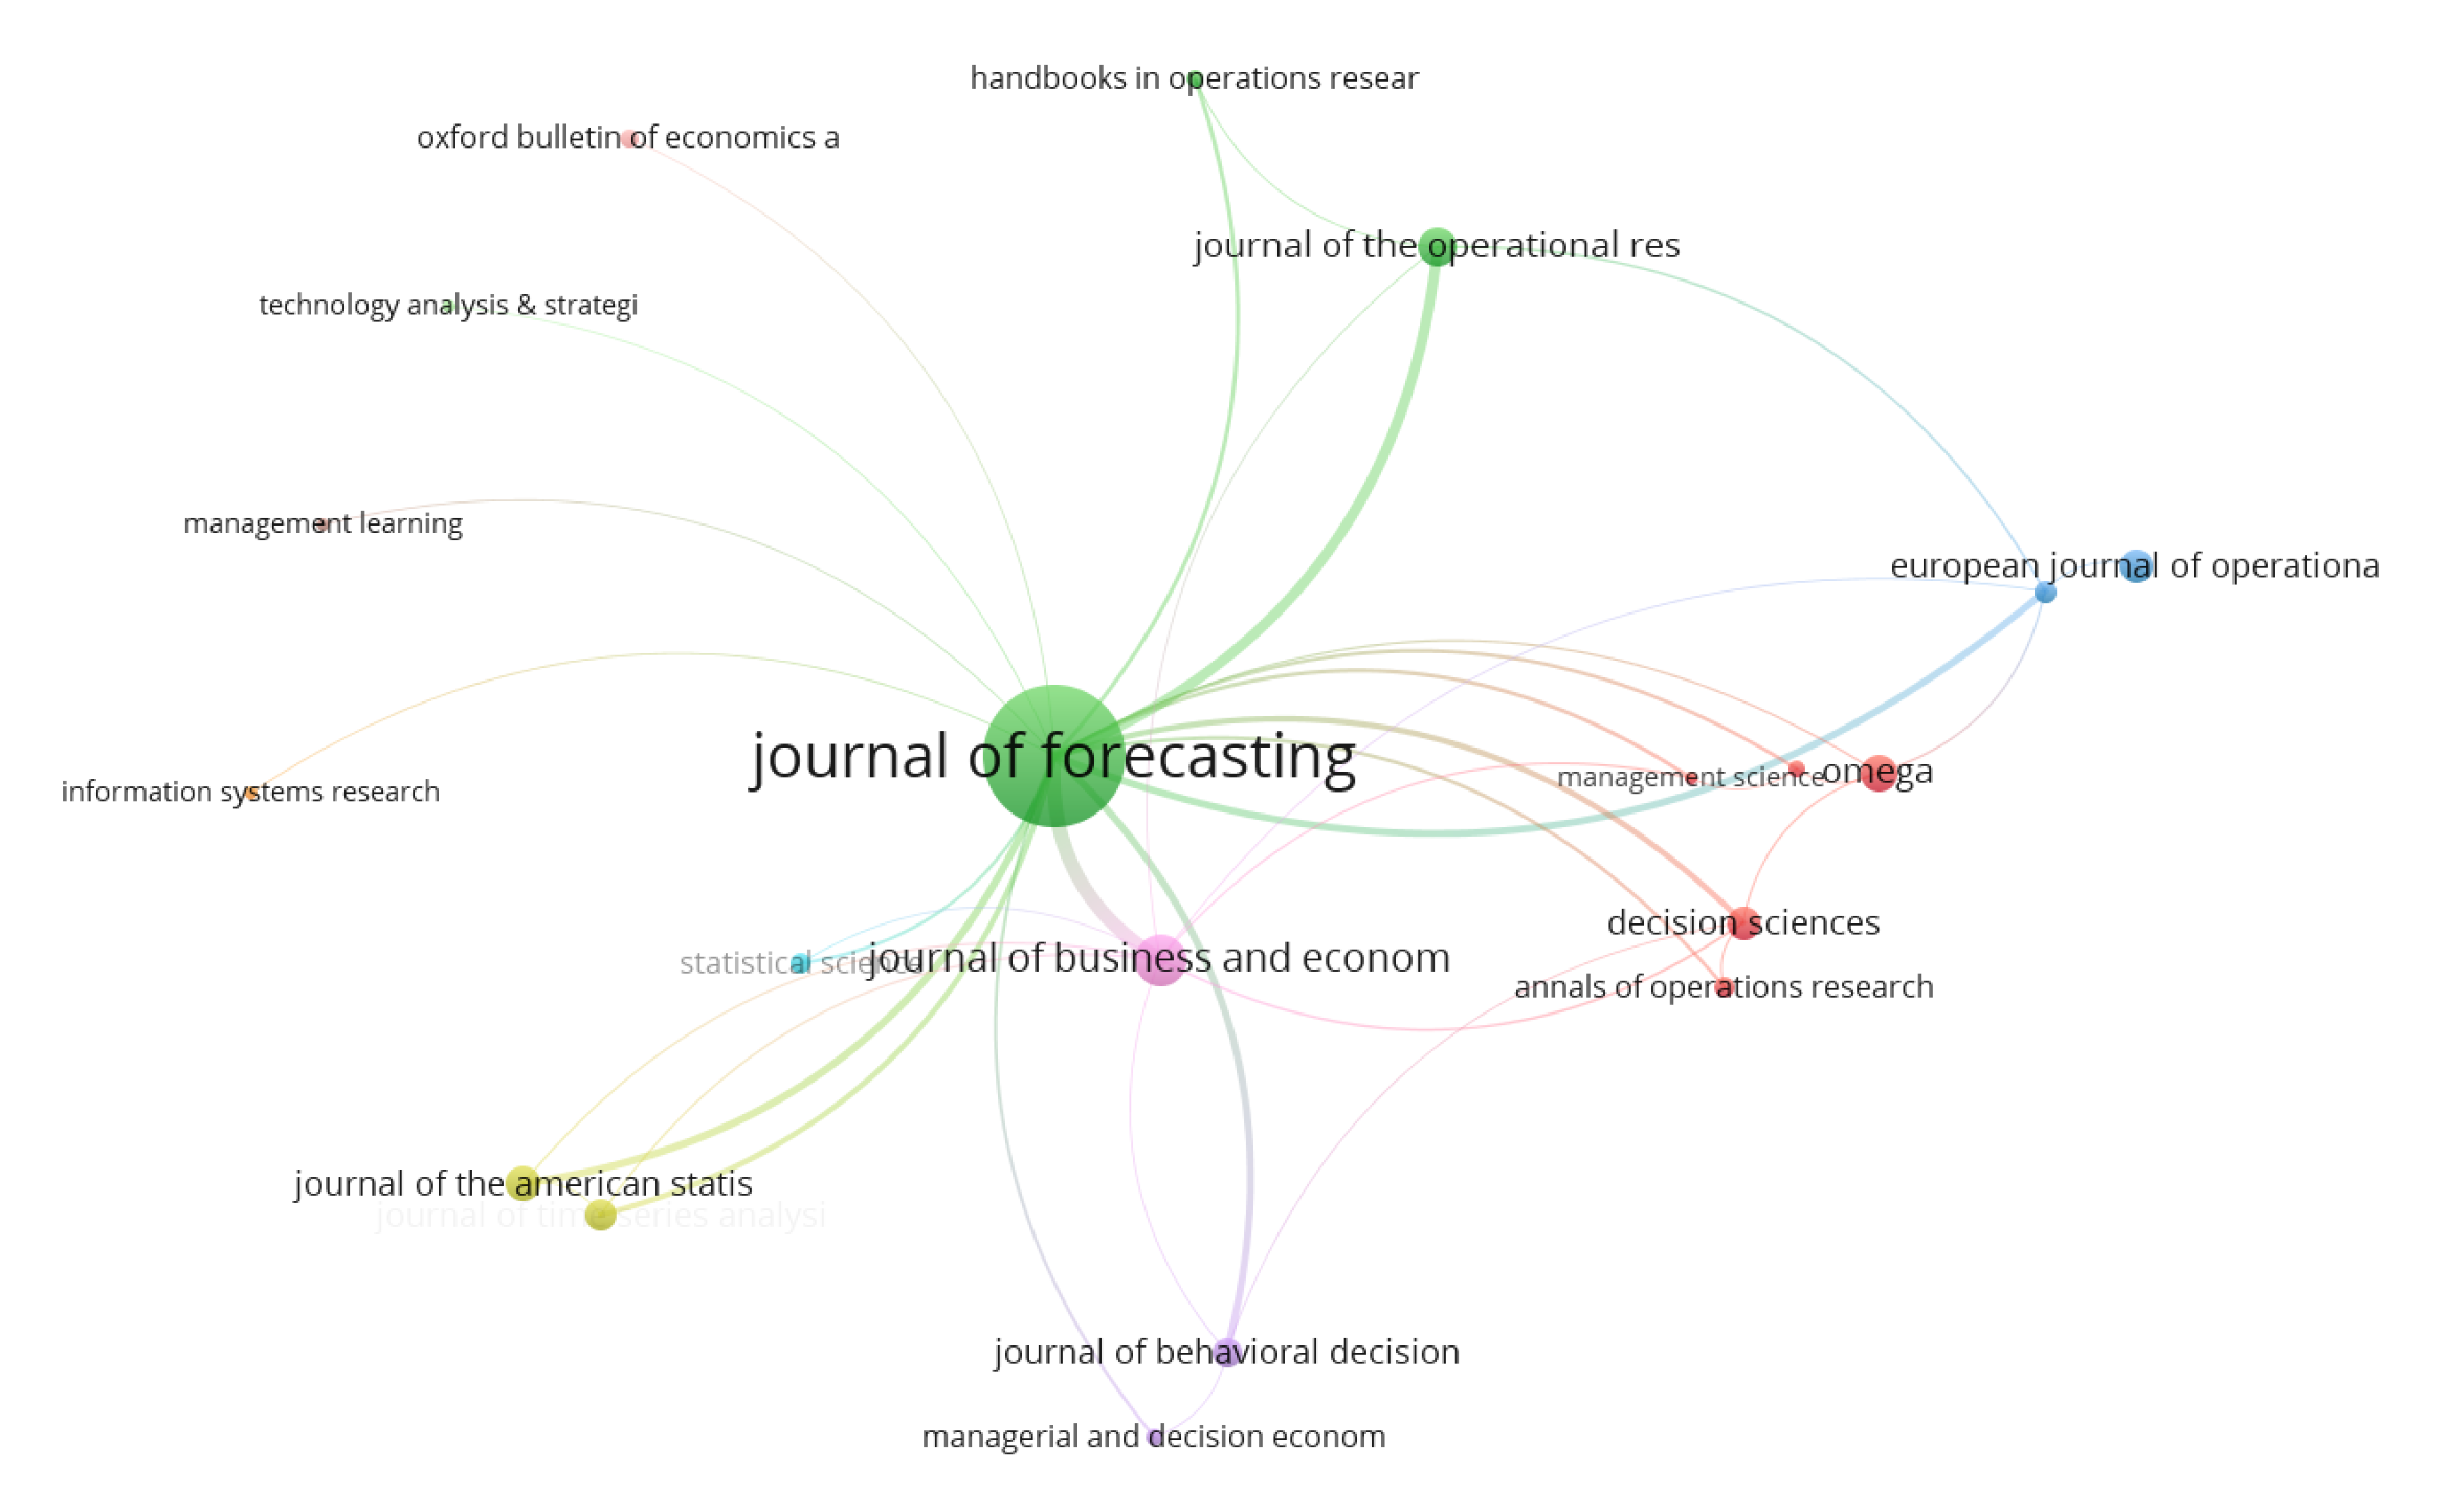
\includegraphics[scale=0.3]{fig.29.eps}
\caption{JF Journal citation network in Decision Science from 1982 to 1994}
\end{figure}

\begin{figure}[htbp]
\centering
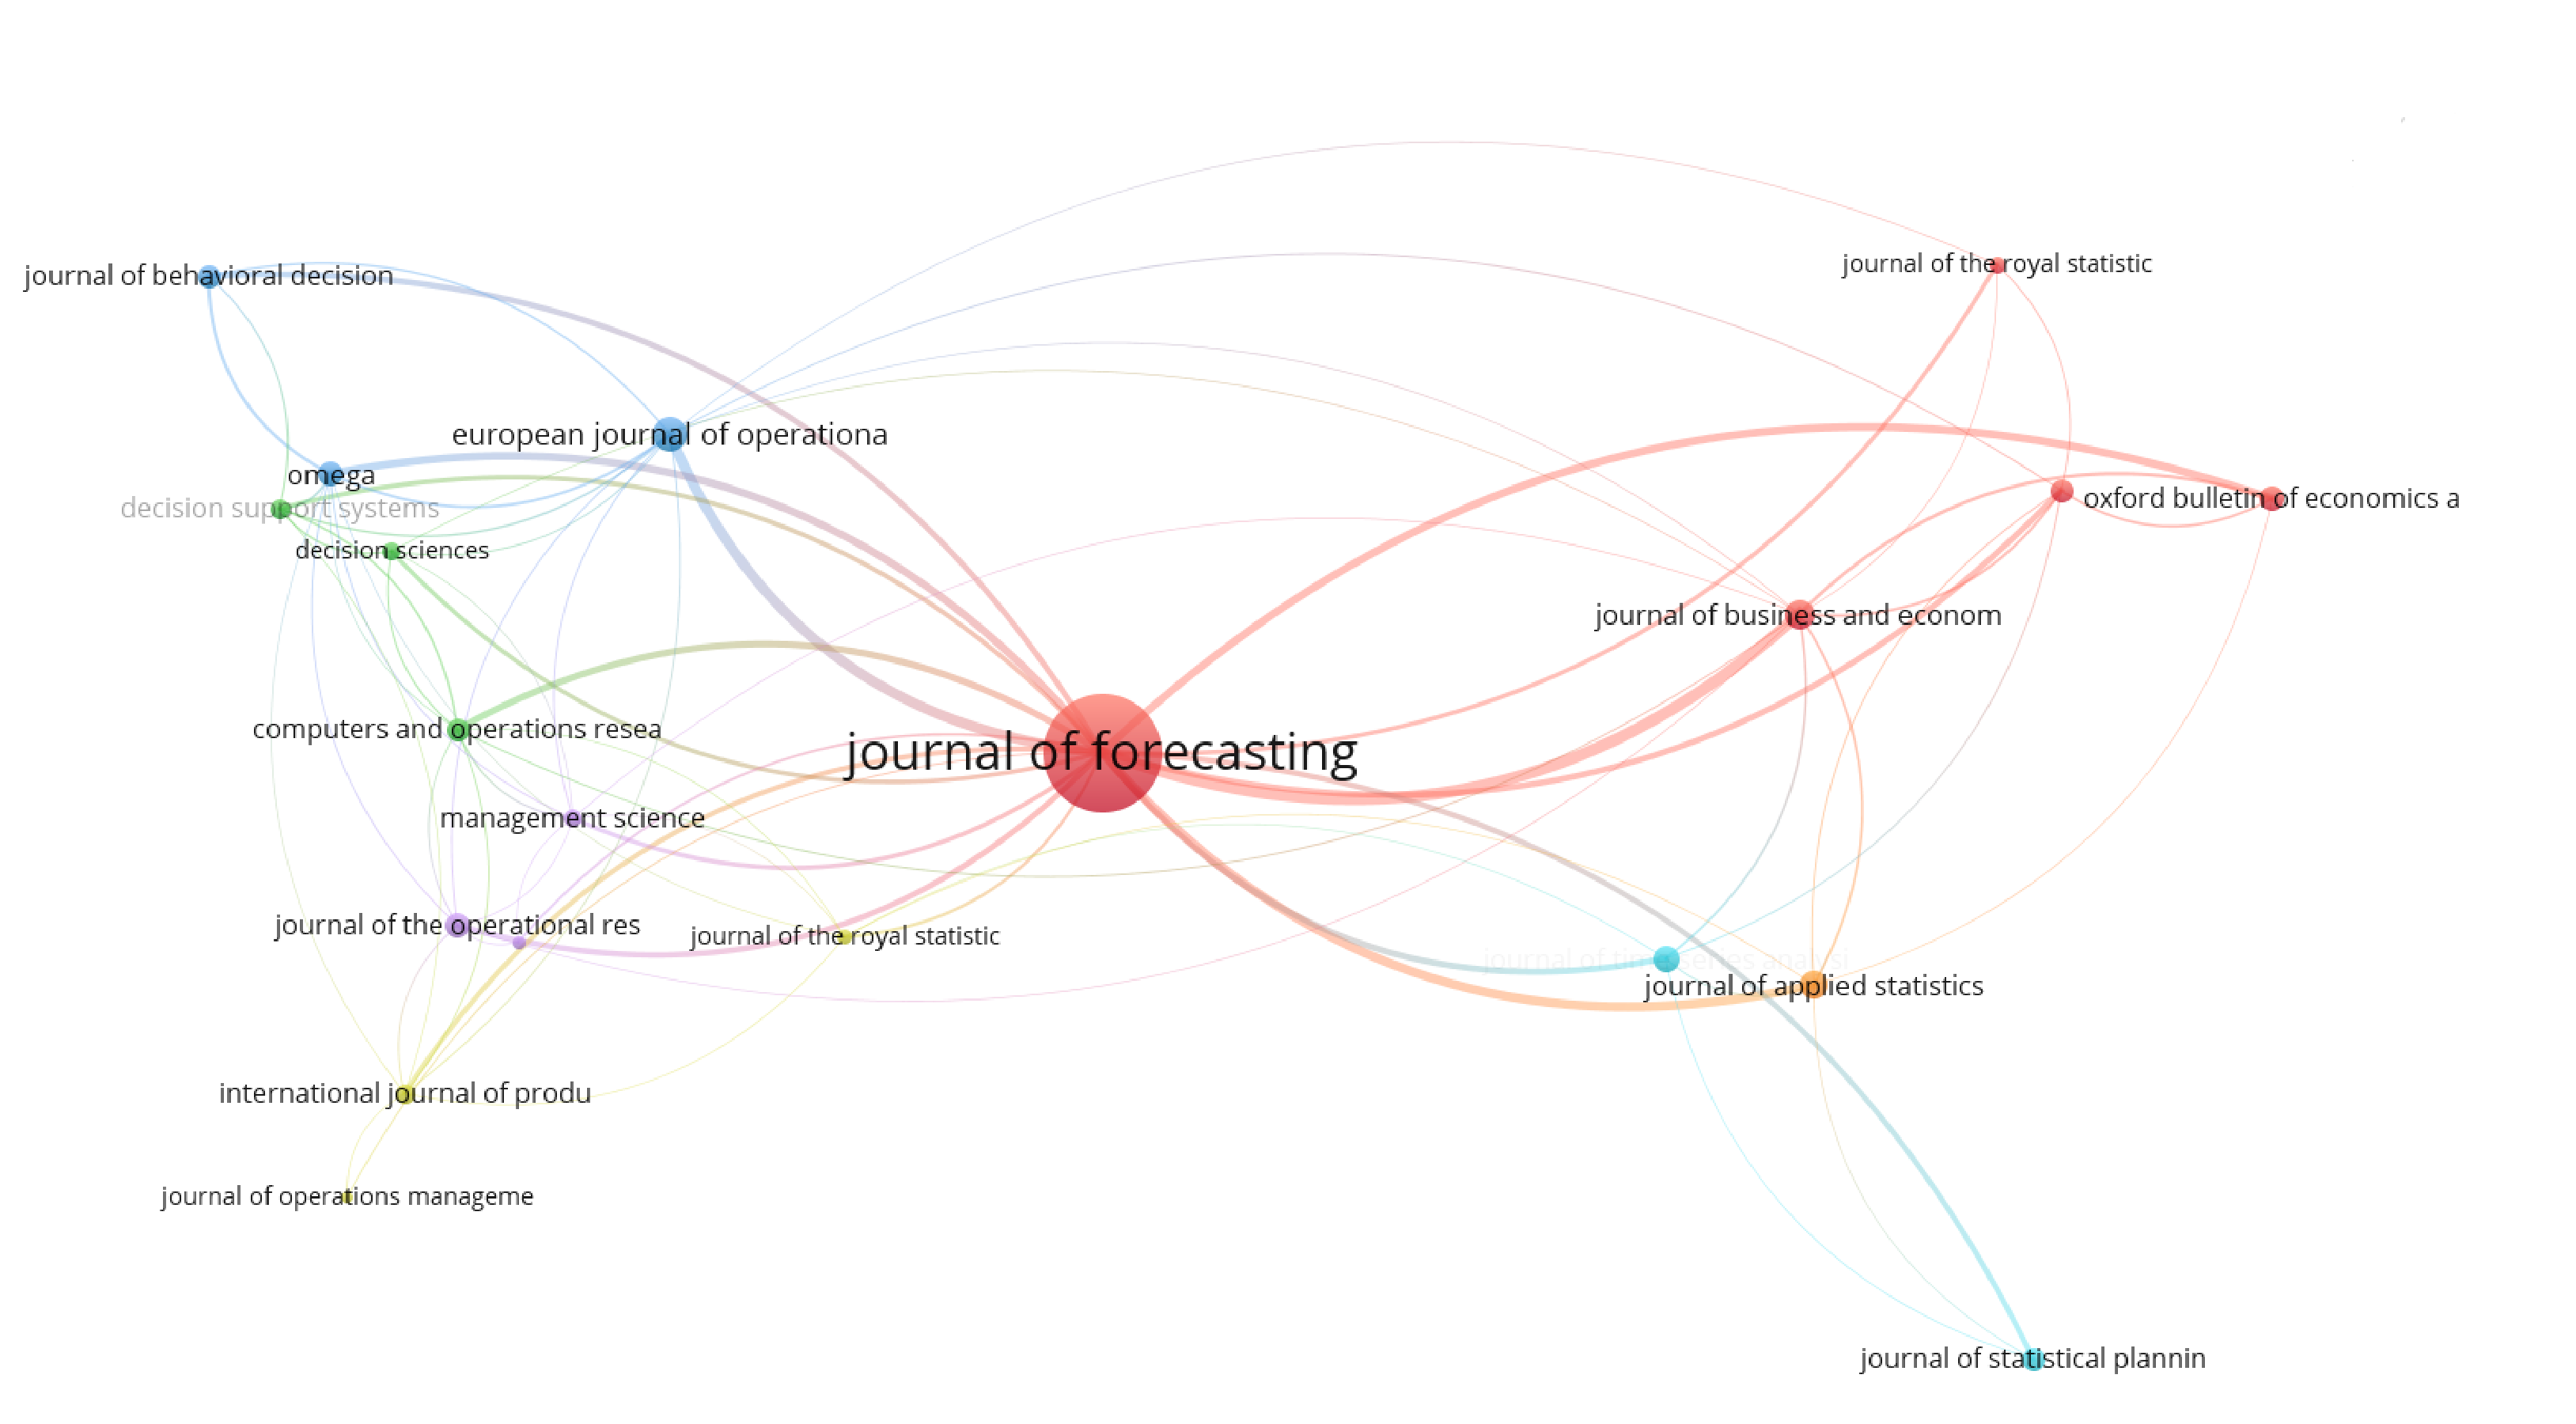
\includegraphics[scale=0.3]{fig.30.eps}
\caption{JF Journal citation network in Decision Science from 1995 to 2007}
\end{figure}

\begin{figure}[htbp]
\centering
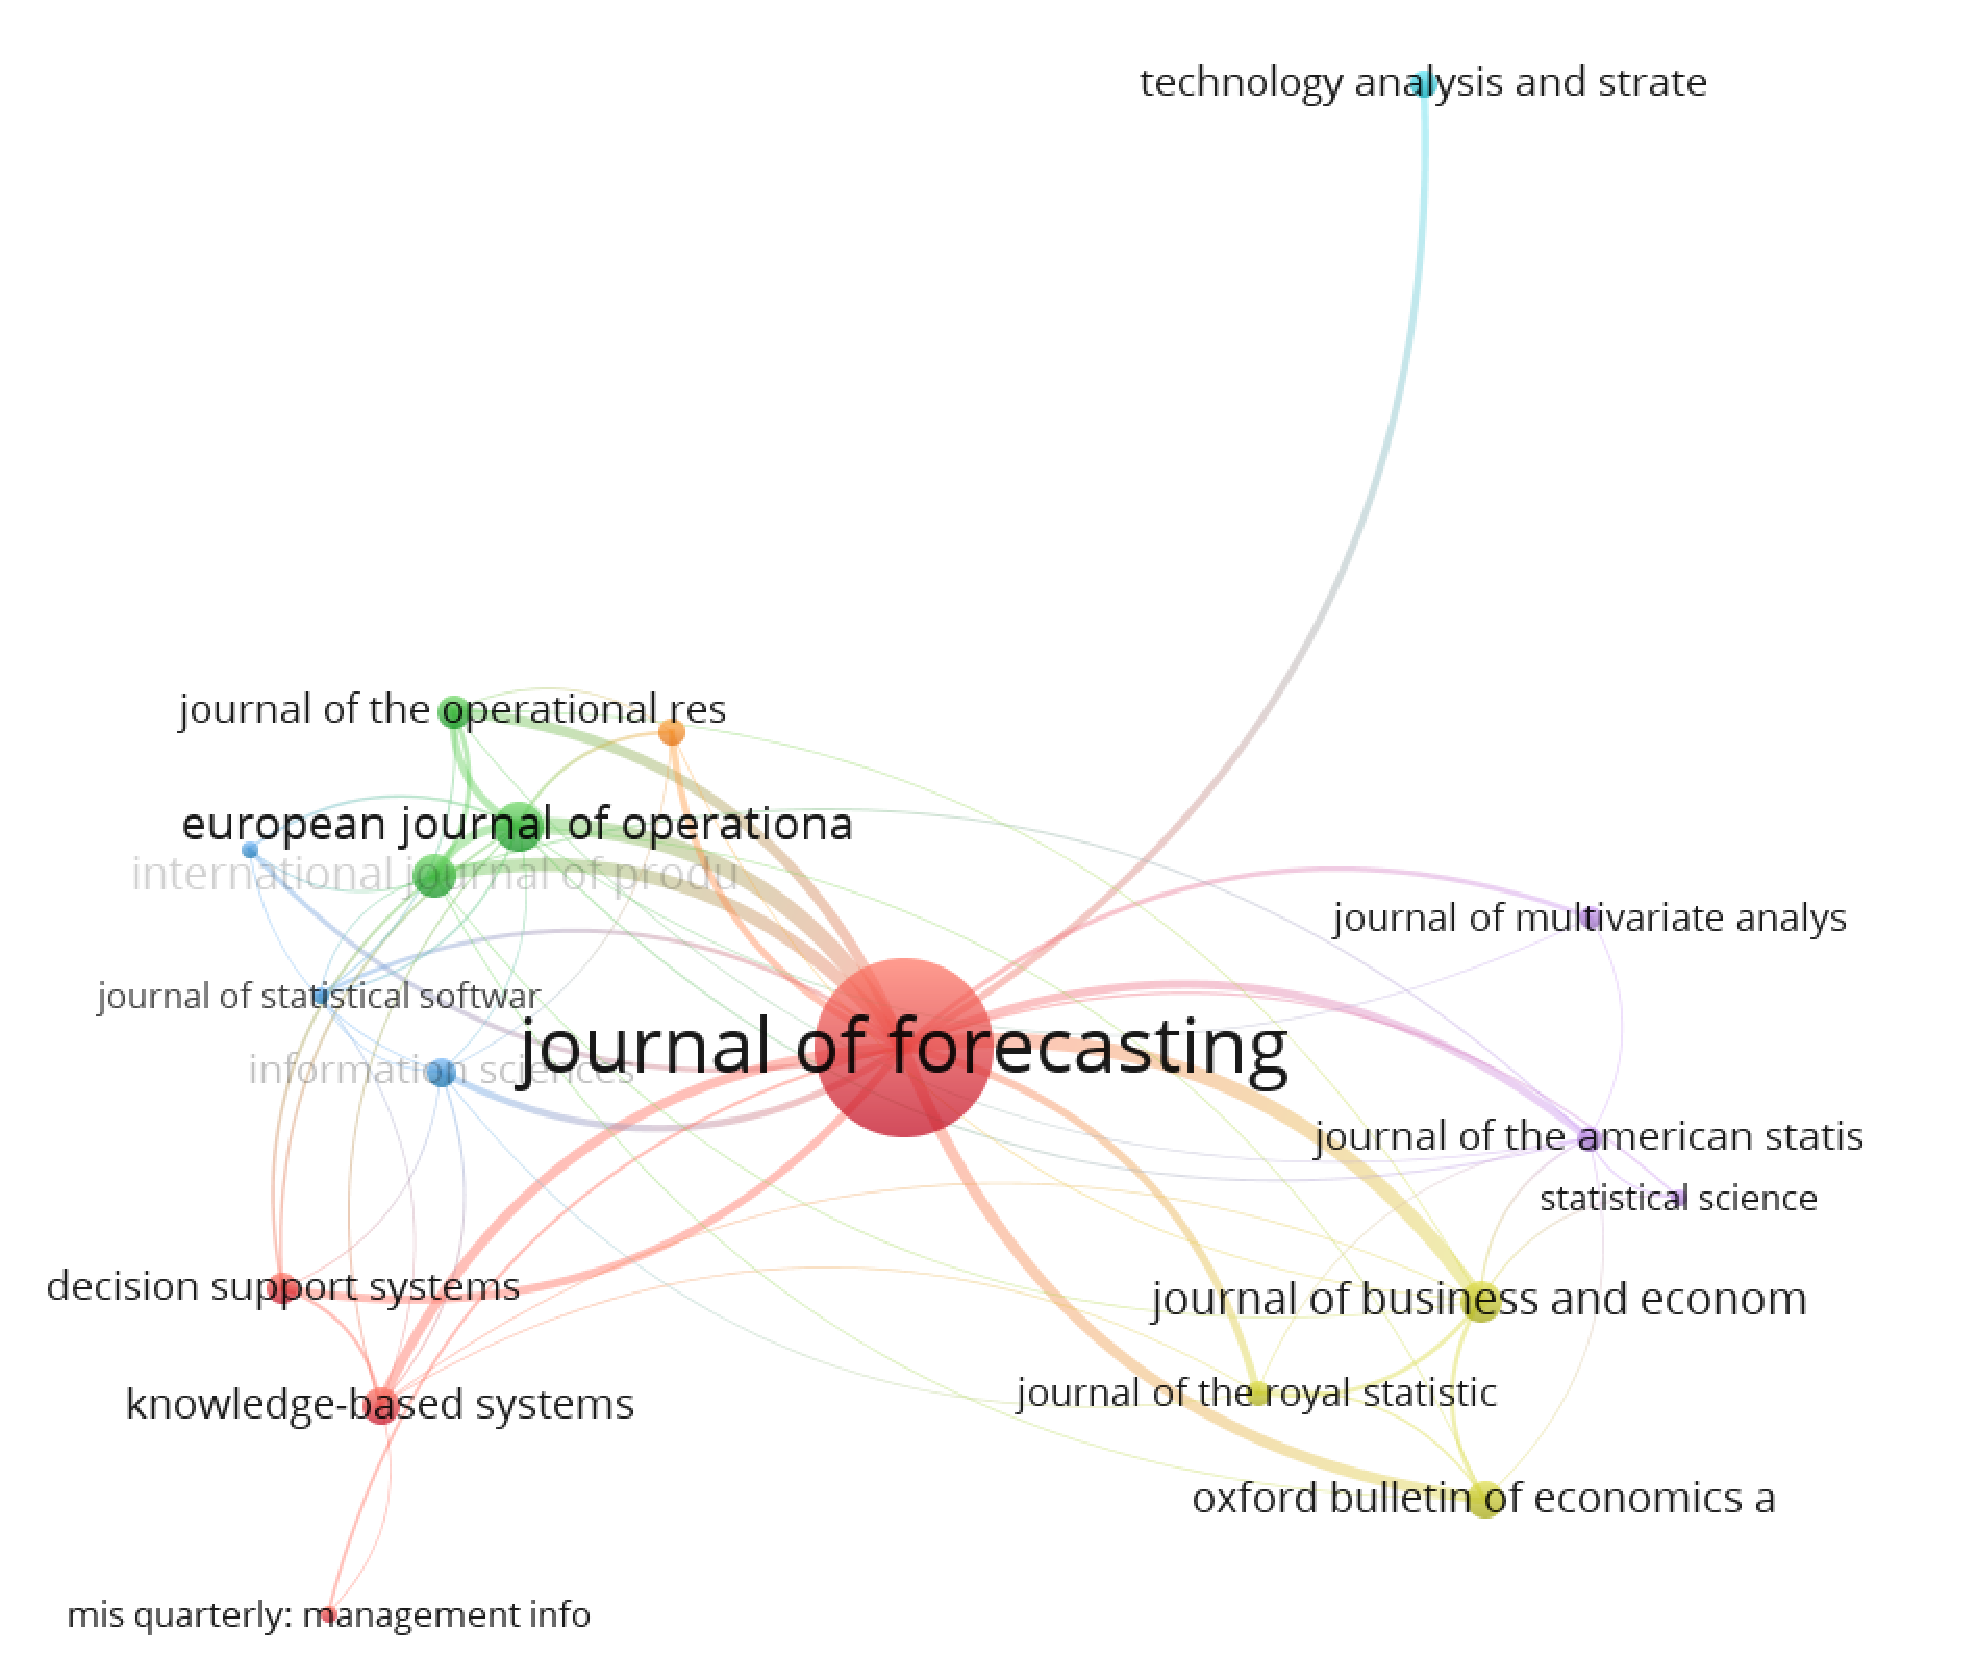
\includegraphics[scale=0.3]{fig.31.eps}
\caption{JF Journal citation network in Decision Science from 2008 to 2019}
\end{figure}

\begin{landscape}
\begin{table}[!htbp]
    \centering
    \caption{The information about the journal citation networks in Decision Science based on the JF citing papers}
    \setlength{\tabcolsep}{0.3mm}{
    \begin{tabular}{p{1.5cm}<{\centering} p{6cm}<{\centering} p{1.5cm}<{\centering}|p{1.5cm}<{\centering} p{6cm}<{\centering} p{1.5cm}<{\centering}|p{1.5cm}<{\centering} p{6cm}<{\centering} p{1.5cm}<{\centering}}
    \hline
        \hline
        \multicolumn{3}{c|}{1985-1996} & \multicolumn{3}{c|}{1997-2008} & \multicolumn{3}{c}{2009-2019}\\
    \hline
    \multicolumn{9}{c}{Limiting condition}\\
    \hline
        \multicolumn{3}{c|}{Number>=1 Citation>=10} & \multicolumn{3}{c|}{Number>=5 Citation>=200} & \multicolumn{3}{c}{Number>=40 Citation>=200}\\
    \hline
    \multicolumn{9}{c}{Parameters}\\
    \hline
    Clusters & Local links & Link strength & Clusters & Local links & Link strength & Clusters & Local links & Link strength\\
    9 & 18 & 173 & 8    & 66 & 1025 & 7 & 168 & 6146\\
        \hline
        \hline
   R & Journal & Links & R & Journal & Links & R & Journal & Links\\
1 & Journal of Business and Economic Statistics & 98 & 1 & Journal of Business and Economic Statistics & 124 & 1 & European Journal of Operational Research & 139\\
2 & Journal of The Operational Research Society & 53 & 2 & European Journal of Operational Research & 96 & 2 & Journal of Business and Economic Statistics & 109\\
3 & Journal of the American Statistical Association & 27 & 3 & Journal of Applied Statistics & 74 & 3 & International Journal of Production Economics & 89\\
4 & Journal of Applied Statistics & 24 & 4 & Oxford Bulletin of Economics and Statistics & 56 & 4 & Oxford Bulletin of Economics and Statistics & 64\\
5 & Journal of Behavioral Decision Making & 24 & 5 & Omega & 53 & 5 & Journal of The Operational Research Society & 55\\
6 & Decision Sciences & 16 & 6 & Computers and Operations Research & 41 & 6 & Knowledge-Based Systems & 50\\
7 & Journal of Time Series Analysis & 15 & 7 & Journal of Time Series Analysis & 35 & 7 & Decision Support Systems & 33\\
8 & Handbooks in Operations Research and Management Science & 8 & 8 & Journal of the American Statistical Association & 33 & 8 & Journal of the American Statistical Association & 33\\
9 & Management Science & 7 & 9 & Journal of Behavioral Decision Making & 31 & 9 & Journal of the Royal Statistical Society. Series A: Statistics In Society & 30\\
10 & Annals of Operations Research & 6 & 10 & Journal of the Operational Research Society & 30 & 10 & Technology Analysis and Strategic Management & 25\\
  \hline
  \hline
    \end{tabular}}
\end{table}
\end{landscape}

\noindent 3.2.2.5. Journal citation network in Psychology

The journal citation relationships between JF papers and their citing
papers belonging to Psychology are depicted in Fig. 32-34. The total
link strength of journal citation network in the period 3 is 218, which
is the weakest in all of the networks in the period 3 across the five
selected subject areas. It denotes that the density of the citation
network in Psychology is the lowest, and the citing journals are not
very closely related. From table 20, we find only two citing journals
(Journal of Behavioral Decision Making, Organizational Behavior and
Human Decision Processes) in the period 1 keep showing in the period 2
and 3. However, another four citing journals (Technological Forecasting
and Social Change, Decision Support Systems, Acta Psychologica, Journal
of Experimental Psychology: Learning Memory and Cognition) in the period
2 are in the list of the period 3, which indicates the knowledge
diffusion starting from JF keeps a continuity ranging from period 2 to
period 3. However, observing from the Fig. 34, a new cluster is emerging
including some cognitive-related journal and decision making-related
journal. These new emerging citing journals are in the citation
relationship with JF, but the distance between them and JF is longer
than others, which demonstrates the content similarity between them and
JF is much lower than other citing journals. The emergence of these
journals denotes the JF researches in the past ten years have attracted
increasing cognitive-related journals and decision making-related
journals, and maybe it is a hot research direction in the forecasting
application in Psychology.

\begin{figure}[htbp]
\centering
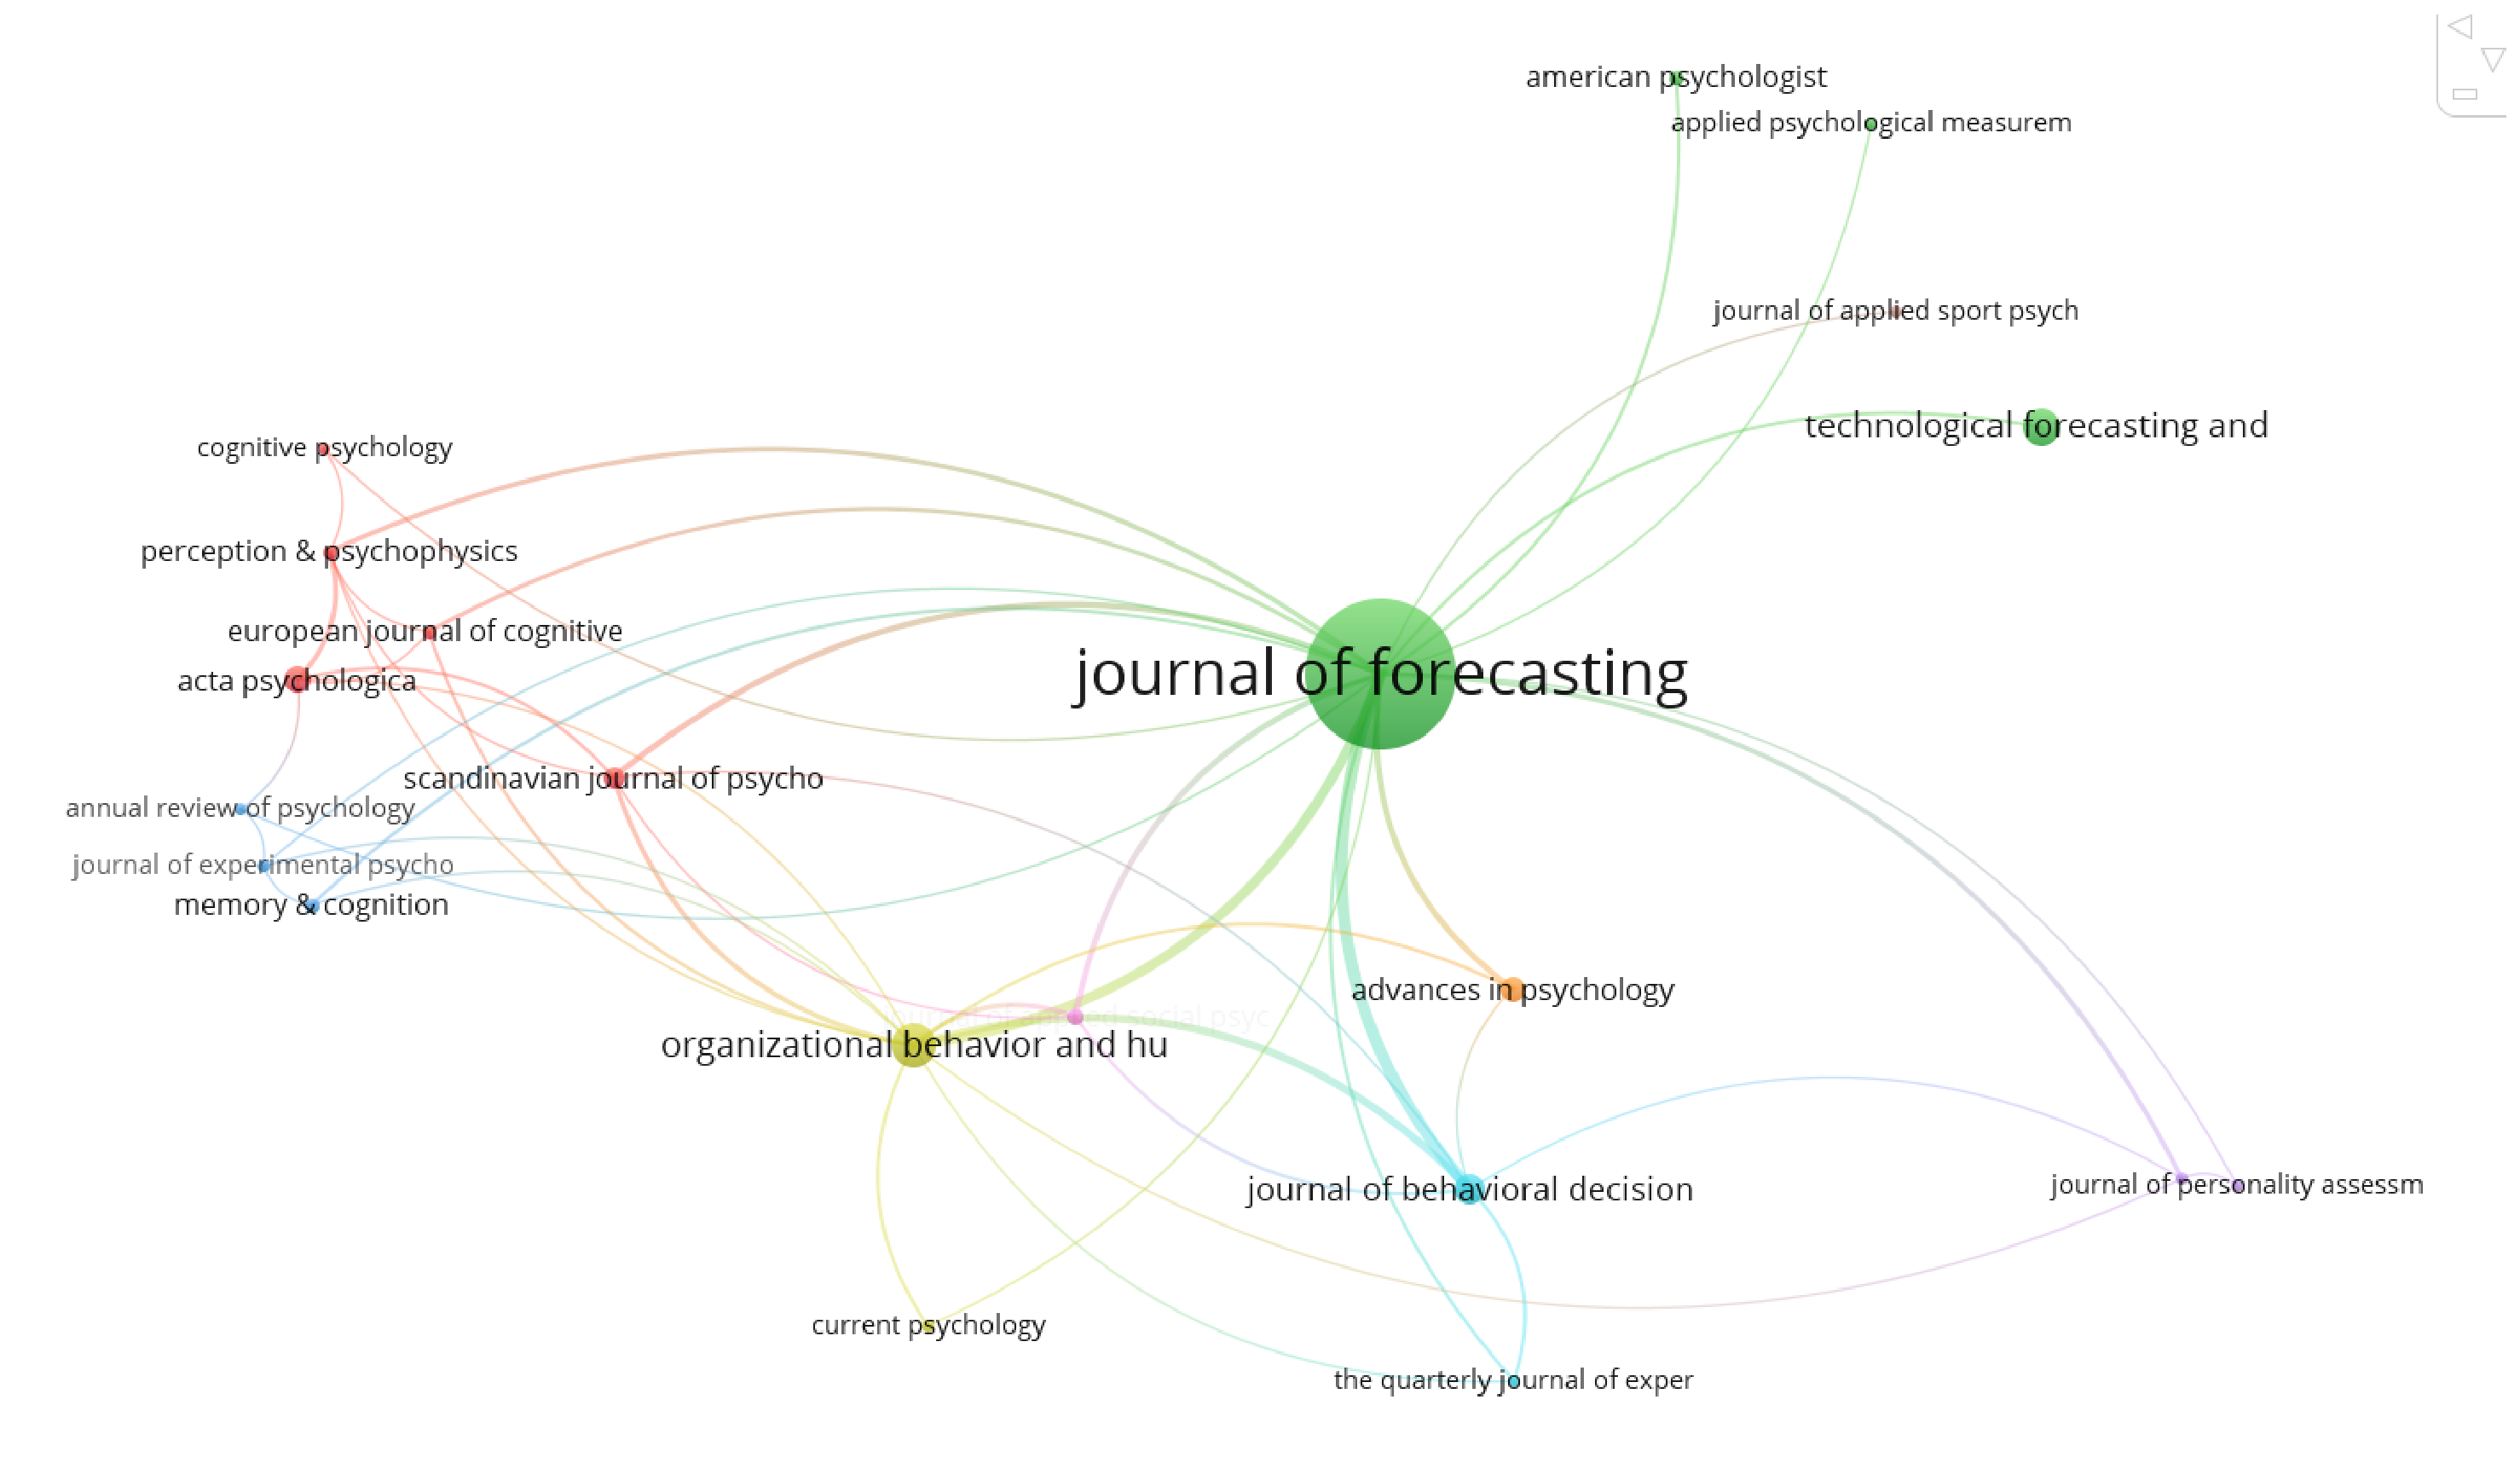
\includegraphics[scale=0.3]{fig.32.eps}
\caption{JF Journal citation network in Psychology from 1982 to 1994}
\end{figure}

\begin{figure}[htbp]
\centering
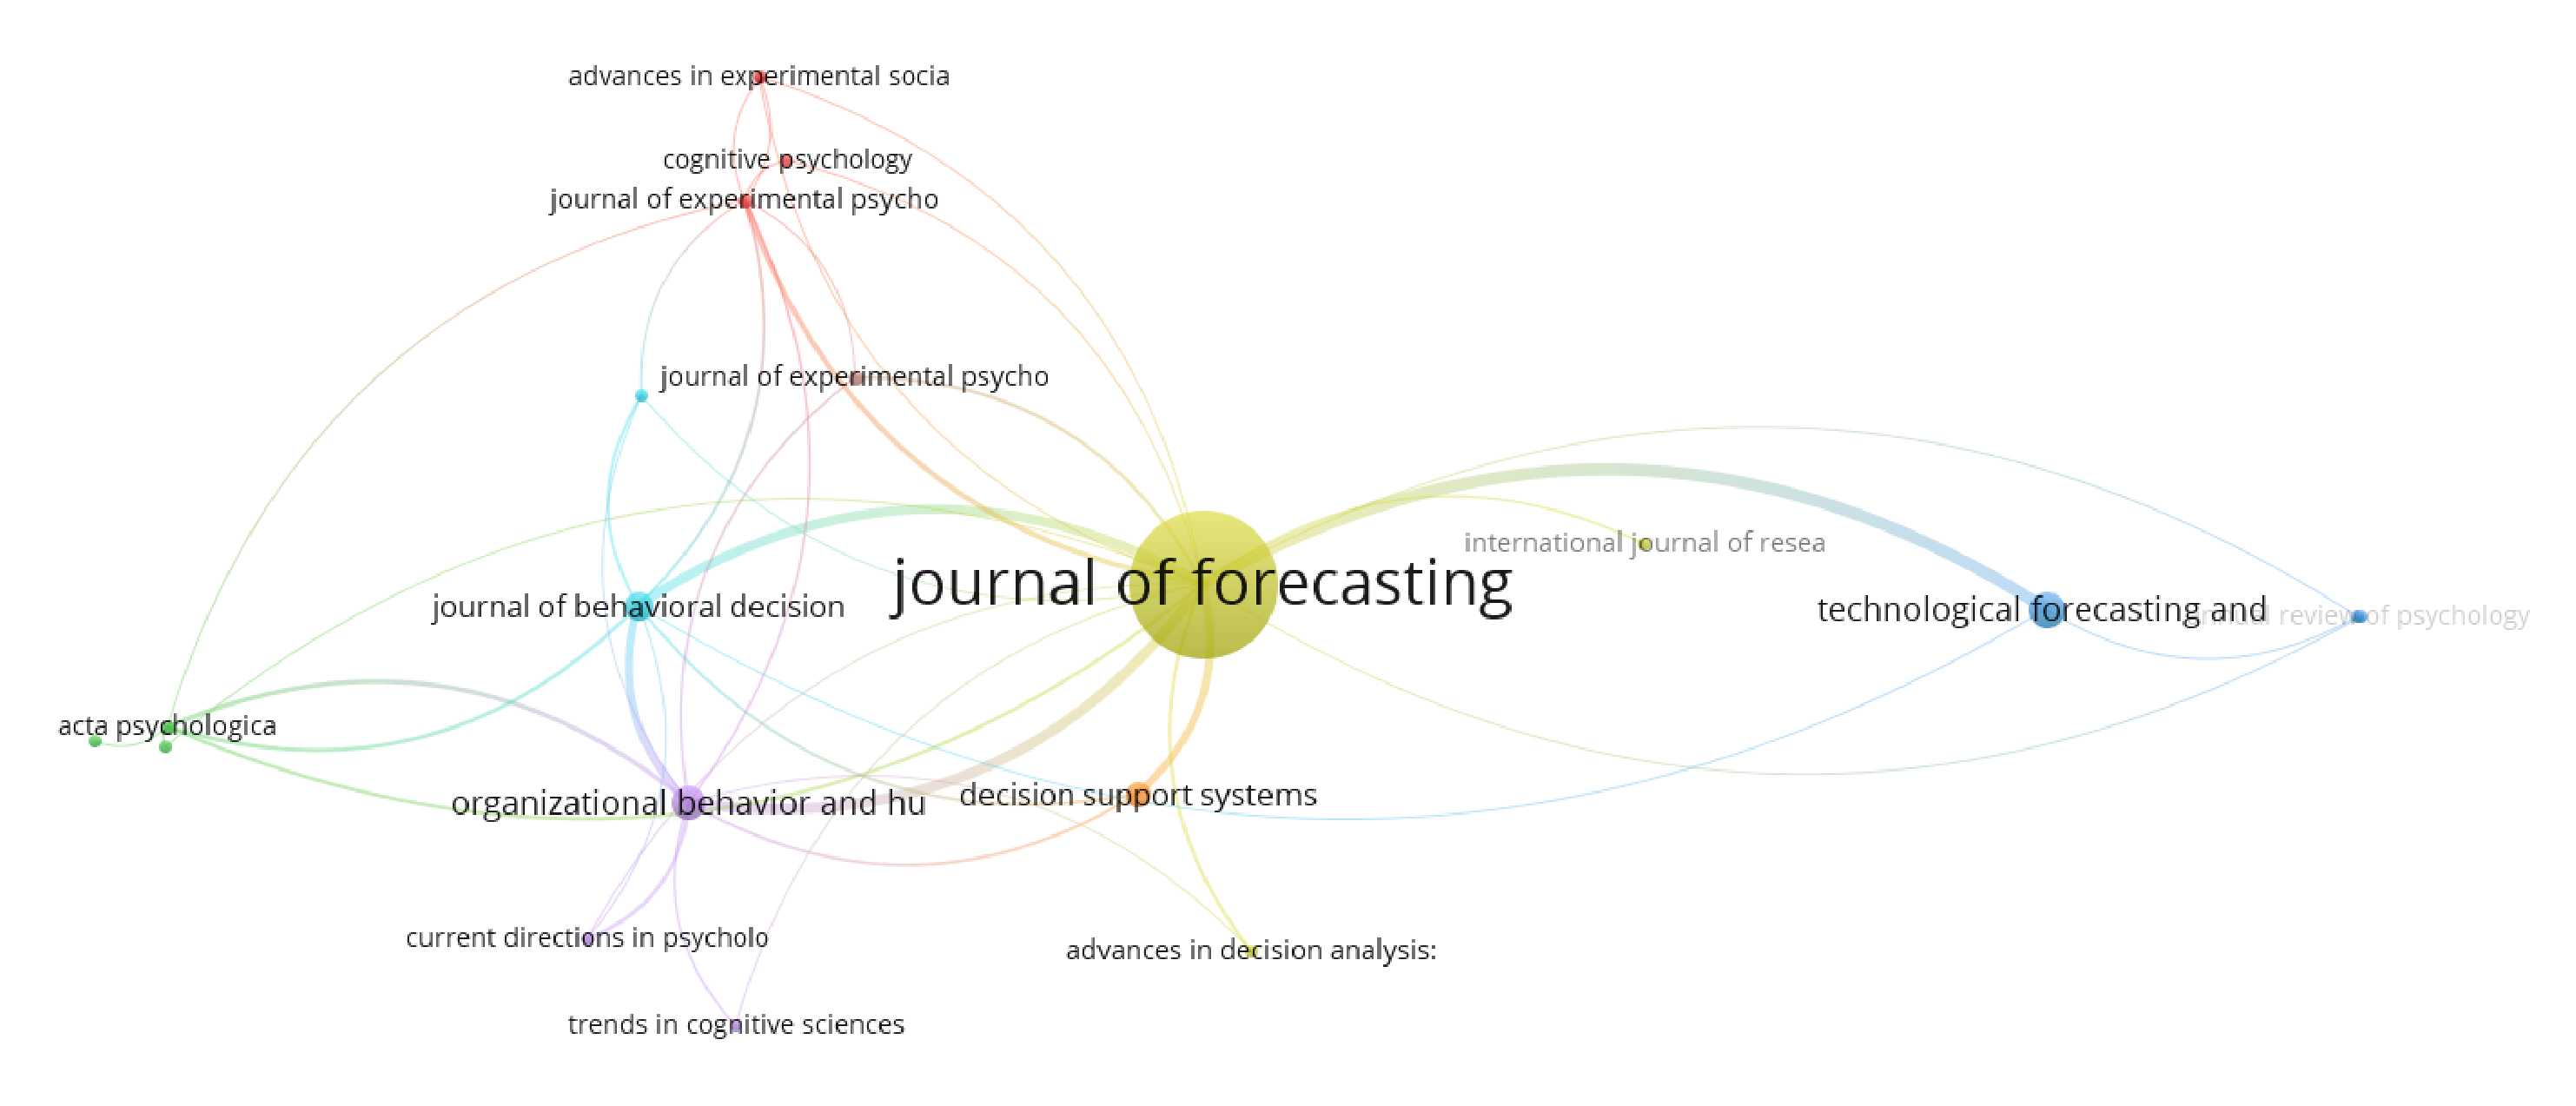
\includegraphics[scale=0.3]{fig.33.eps}
\caption{JF Journal citation network in Psychology from 1995 to 2007}
\end{figure}

\begin{figure}[htbp]
\centering
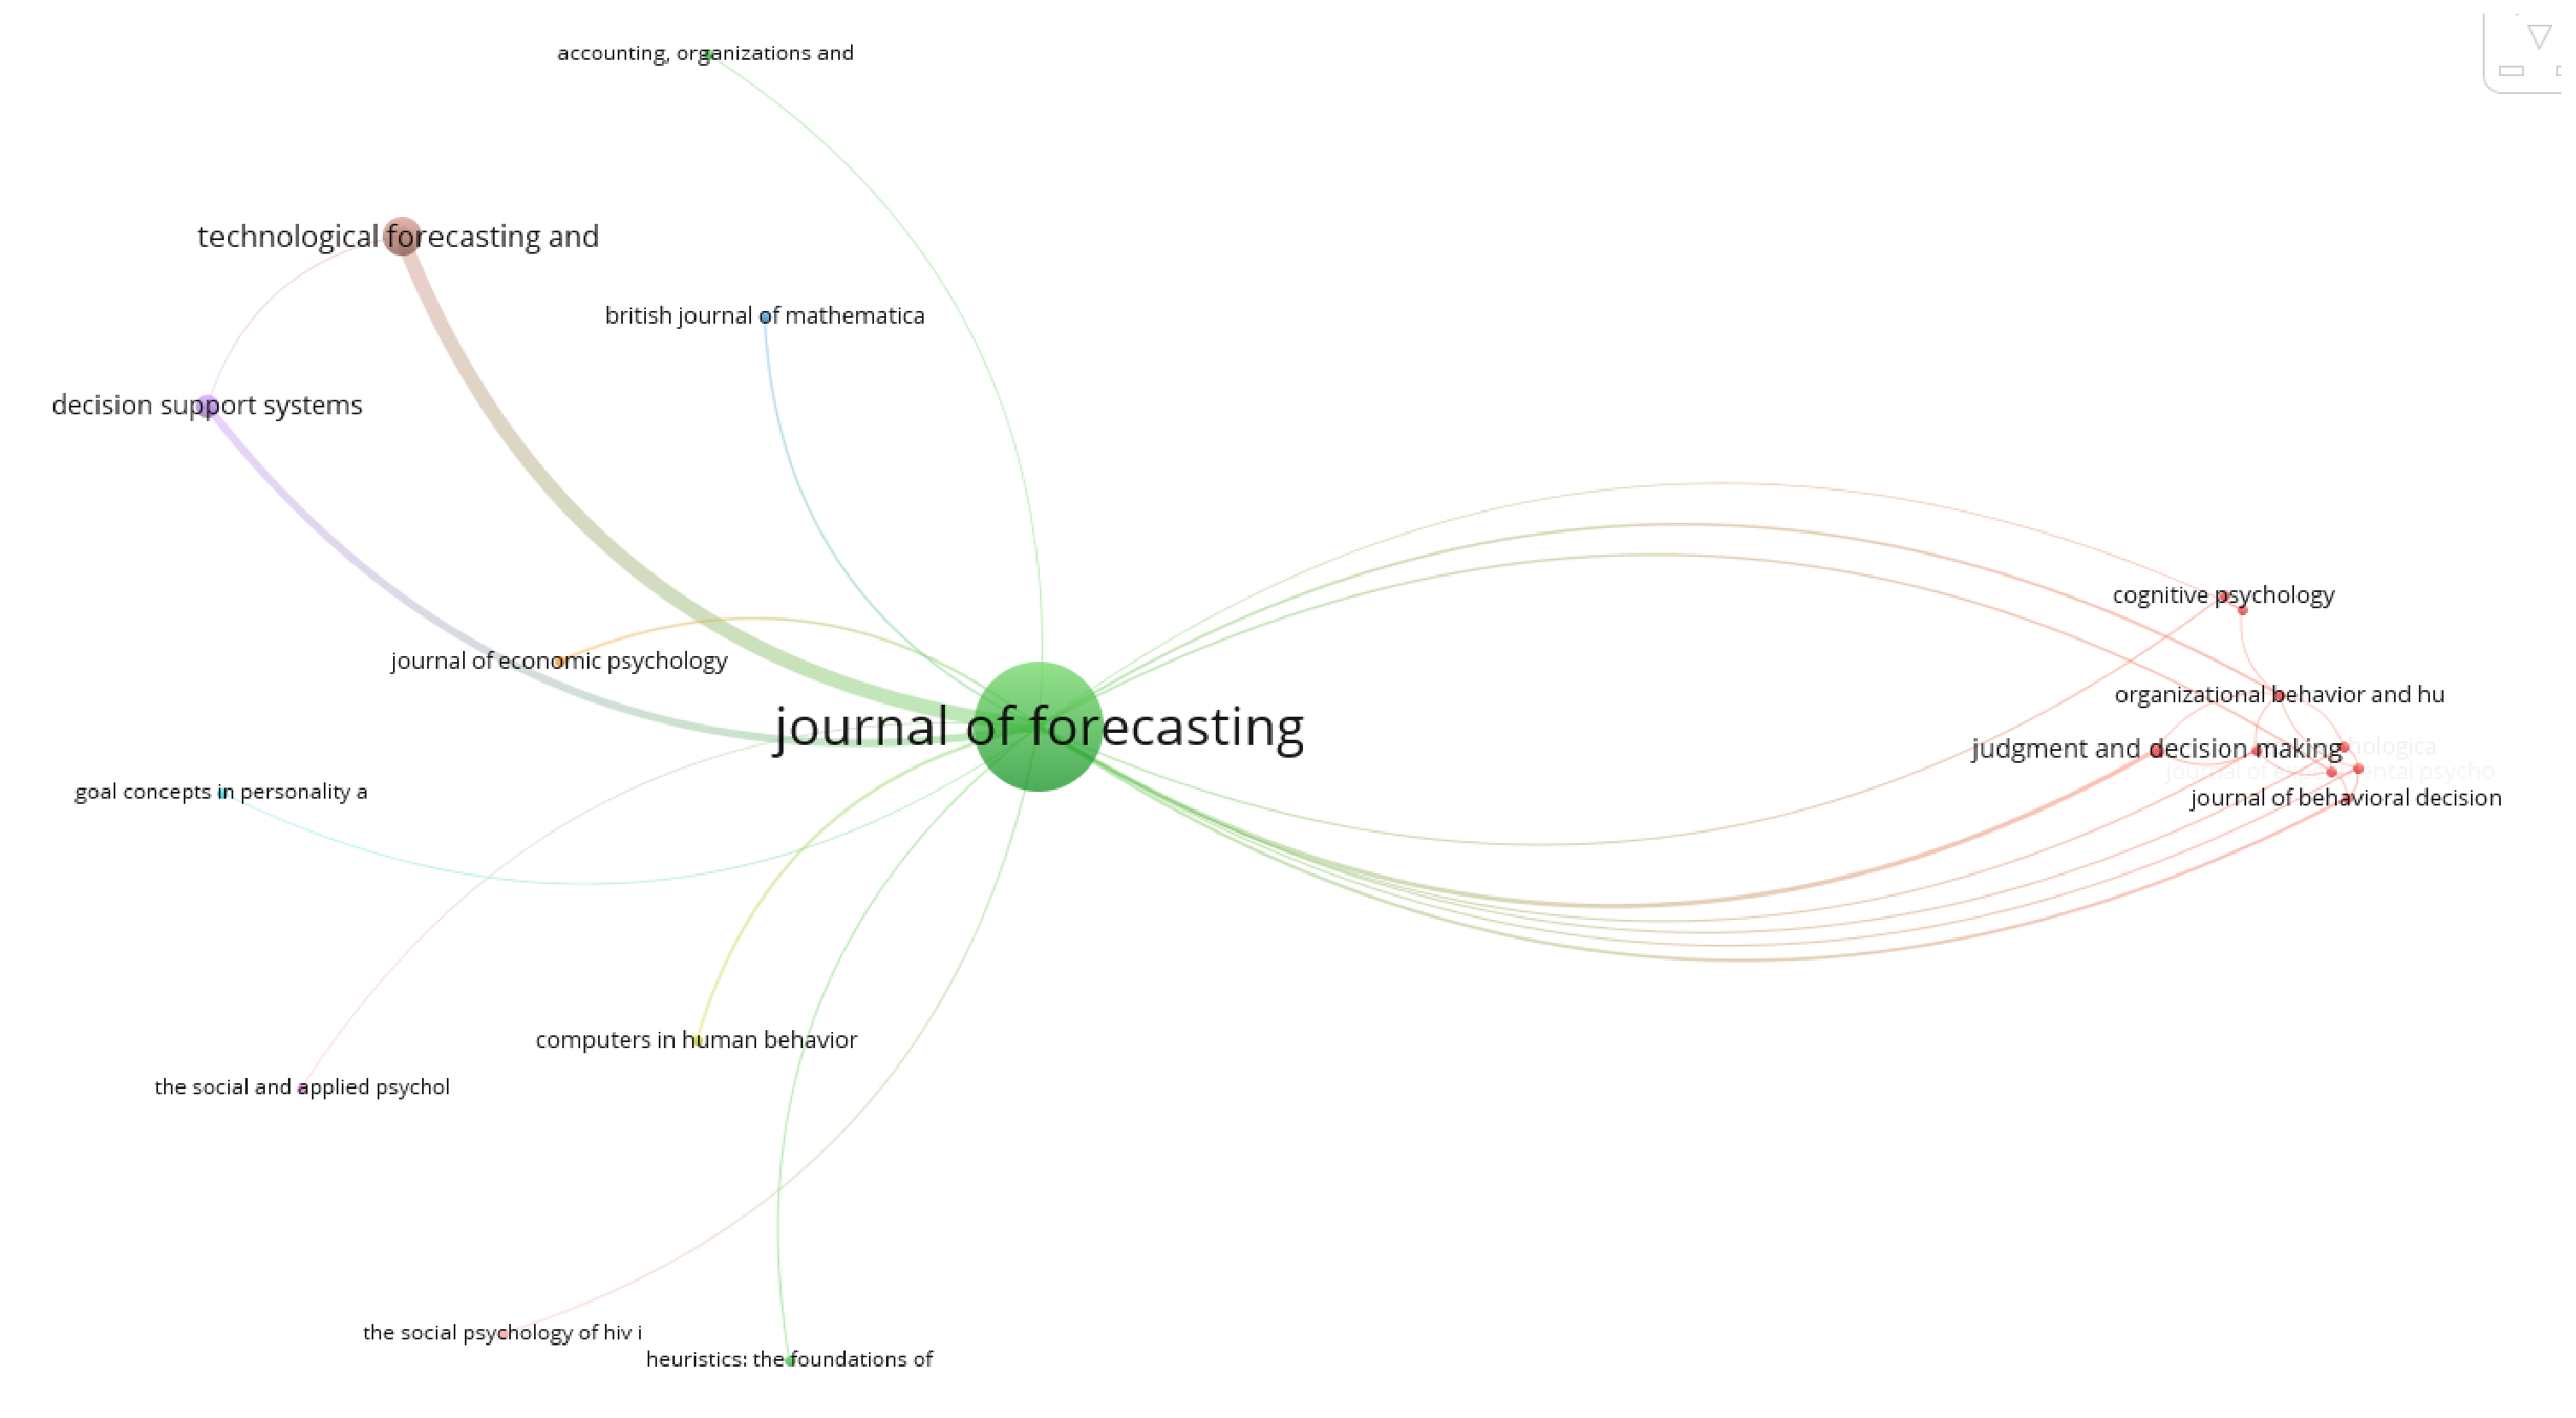
\includegraphics[scale=0.3]{fig.34.eps}
\caption{ JF Journal citation network in Psychology from 2008 to 2019}
\end{figure}

\begin{landscape}
\begin{table}[!htbp]
    \centering
    \caption{ The information about the journal citation networks in Psychology based on the JF citing papers}
    \setlength{\tabcolsep}{0.3mm}{
    \begin{tabular}{p{1.5cm}<{\centering} p{6cm}<{\centering} p{1.5cm}<{\centering}|p{1.5cm}<{\centering} p{6cm}<{\centering} p{1.5cm}<{\centering}|p{1.5cm}<{\centering} p{6cm}<{\centering} p{1.5cm}<{\centering}}
    \hline
        \hline
        \multicolumn{3}{c|}{1985-1996} & \multicolumn{3}{c|}{1997-2008} & \multicolumn{3}{c}{2009-2019}\\
    \hline
    \multicolumn{9}{c}{Limiting condition}\\
    \hline
        \multicolumn{3}{c|}{Number>=1 Citation>=10} & \multicolumn{3}{c|}{Number>=5 Citation>=200} & \multicolumn{3}{c}{Number>=40 Citation>=200}\\
    \hline
    \multicolumn{9}{c}{Parameters}\\
    \hline
    Clusters & Local links & Link strength & Clusters & Local links & Link strength & Clusters & Local links & Link strength\\
    9 & 18 & 173 & 8    & 66 & 1025 & 7 & 168 & 6146\\
        \hline
        \hline
   R & Journal & Links & R & Journal & Links & R & Journal & Links\\
1 & Journal of Behavioral Decision Making & 24 & 1 & Technological Forecasting and Social Change & 49 & 1 & Technological Forecasting and Social Change & 118\\
2 & Organizational Behavior and Human Decision Processes & 17 & 2 & Organizational Behavior and Human Decision Processes & 37 & 2 & Decision Support Systems & 33\\
3 & Advances in Psychology & 6 & 3 & Journal of Behavioral Decision Making & 31 & 3 & Judgment and Decision Making & 11\\
4 & Journal of Applied Social Psychology & 6 & 4 & Decision Support Systems & 20 & 4 & Computers in Human Behavior & 5\\
5 & Scandinavian Journal of Psychology & 6 & 5 & Journal of Experimental Psychology: Applied & 9 & 5 & Journal of Behavioral Decision Making & 5\\
6 & Perception \& Psychophysics & 4 & 6 & Acta Psychologica & 4 & 6 & Journal of Economic Psychology & 4\\
7 & Psychological Bulletin & 4 & 7 & Advances in Decision Analysis: From Foundations to Applications & 4 & 7 & Organizational Behavior and Human Decision Processes & 4\\
8 & European Journal of Cognitive Psychology & 3 & 8 & Journal of Experimental Psychology: Learning Memory and Cognition & 4 & 8 & British Journal of Mathematical and Statistical Psychology & 3\\
9 & American Psychologist & 2 & 9 & international Journal of Research in Marketing & 2 & 9 & Journal of Experimental Psychology: Learning Memory and Cognition & 3\\
10 & Memory \& Cognition & 2 & 10 & Advances in Experimental Social Psychology & 1 & 10 & Acta Psychologica & 2\\
  \hline
  \hline
    \end{tabular}}
\end{table}
\end{landscape}

\subsubsection{Knowledge diffusion of IJF outside the forecasting
field}\label{knowledge-diffusion-of-ijf-outside-the-forecasting-field}

Knowledge diffusion of the forecasting field has been investigated via
constructing journal citation networks of IJF papers, JF papers, and
their citing papers. Predefined subject areas are used to categorize
papers. Four subject areas in IJF and five subject areas in JF, which
have a remarkable performance in knowledge diffusion has been further
investigated through analyzing journal citation relationships. Based on
the results in subsection 3.2.2, some contributing journals can be
obtained, but important papers that have a significant impact on these
journals are still undetermined. Therefore, in this subsection, the top
ten IJF citing journals and JF citing journals in each subject area are
crossed to derive the citing journals both appear in the list of IJF and
JF. Then the citing journals of the crossing result are considered to be
the most contributing citing journals of forecasting field in each
subject area. Note that only citing journals in the period 3 are
considered because we focus on the emerging contributing citing journals
in the past ten years. Finally, we derive six contributing journals in
Computer Science, eight contributing journals in Engineering, six
contributing journals in Decision Science, and eight in Psychology.
According to the data in different subject areas, different limiting
conditions are set. In Computer Science and Engineering, IJF papers that
are cited by at least six contributing journals are selected. In
Decision Science and Psychology, IJF papers that are cited by at least
four contributing journals are selected. All the qualified IJF papers
are harvested and listed in table 21-24.

The above four subject areas are involved in the entire development of
IJF and JF, therefore, we analyze them as the typical subject areas that
integrate the knowledge from the forecasting field. One subject area
includes various journals which have different scopes and research
focuses. If an IJF paper is cited by more journals within the same
subject area, then the knowledge starting from this IJF paper spreads
over a wider range within the subject area. Therefore, we extract papers
that are cited by more journals within one subject area, and in
different subject area, different limiting conditions are set. in table
21, five qualified papers are cited by six journals, and two of five
(Taylor, Menezes, and Mcsharry 2006; Darbellay and Slama 2000) are
related to the forecasting research on electricity demand, which denotes
electricity demand forecasting is a widely-discussed topic in Computer
Science. Another popular topic is the research of forecast accuracy
because two papers focus on it (Hyndman and Koehler 2006; Makridakis
1993). In Engineering, there are three IJF papers cited by six journals,
three IJF papers cited by seven journals, and four IJF papers cited by
eight journals. Two of the ten papers focus on the forecasting
application in neural networks (Zhang, Patuwo, and Hu 1998; Hippert,
Bunn, and Souza 2005). The two papers related to the research of
forecast accuracy (Hyndman and Koehler 2006; Makridakis 1993) which are
cited by the journals in Computer Science also cited by journals in
Engineering. Besides, there are two reviews which research on time
series forecasting and forecasting the diffusion of innovation (Gooijer
and Hyndman 2006; Meade and Islam 2006). In Decision Science, most IJF
papers are cited by four journals. However, one paper is cited by six
journals, and it is the serial research about the well-known
M-Competitions organized by forecasting experts (Makridakis and Hibon
2000). In Psychology, human judgment which affects the forecasting
accuracy is a popular research, and there are three IJF papers focus on
judgmental forecasting in table 24. The first one is a review describing
the development progress of judgmental forecasting over 25 years
(Lawrence et al. 2006). The second one investigates the effects of
judges' forecasting based on two experiments, and discusses whether the
forecasting results would be impaired if the judges have previously made
their own forecasts for the same outcomes (N. Harvey and Harries 2004).
The third one is about the judgmental aggregation strategies, and
discusses the differences between aggregating opinions and choosing one
single judge (Soll and Mannes 2011).

\begin{landscape}
\begin{table}[!htbp]
    \centering
    \caption{Information about the IJF paper cited by the most contributing citing journals in Computer Science}
    \setlength{\tabcolsep}{1mm}{
    \begin{tabular}{p{9cm}<{\centering} p{7cm}<{\centering} p{9cm}<{\centering}p{1cm}<{\centering}}
    \hline
    Paper & Author (year) & Cited by contributing journals & TC\\
  \hline
  Another look at measures of forecast accuracy & Hyndman R.J. and Koehler A.B. (2006) & ASCJ, CSDA, EJOR, LNCS, NC, PIJCNN & 1210\\
Combining forecasts: A review and annotated bibliography & Clemen R.T. (1989) & ASCJ, CSDA, EJOR, LNCS, NC, PIJCNN & 1107\\
A comparison of univariate methods for forecasting electricity demand up to a day ahead & Taylor J.W. et al. (2006) & ASCJ, CSDA, EJOR, LNCS, NC, PIJCNN & 267\\
Accuracy measures: theoretical and practical concerns & Makridakis S. (1993) & ASCJ, CSDA, EJOR, LNCS, NC, PIJCNN & 214\\
Forecasting the short-term demand for electricity: Do neural networks stand a better chance? & Darbellay G.A. and Slama M. (2000) & ASCJ, CSDA, EJOR, LNCS, NC, PIJCNN & 208\\
  \hline
    \end{tabular}}
\end{table}

\begin{table}[!htbp]
    \centering
    \caption{Information about the IJF paper cited by the most contributing citing journals in Engineering}
    \setlength{\tabcolsep}{1mm}{
    \begin{tabular}{p{9cm}<{\centering} p{7cm}<{\centering} p{9cm}<{\centering}p{1cm}<{\centering}}
    \hline
    Paper & Author (year) & Cited by contributing journals & TC\\
  \hline
  Forecasting with artificial neural networks: The state of the art & Zhang G. et al. (1998) & AE, Energies, Energy, ESWA, IEEE-TPS, IJPE, IJPR, MPE & 2022\\
Another look at measures of forecast accuracy & Hyndman R.J. and Koehler A.B. (2006) & AE, Energies, Energy, ESWA, IEEE-TPS, IJPE, IJPR, MPE & 1210\\
Combining forecasts: A review and annotated bibliography & Clemen R.T. (1989) & AE, Energies, Energy, ESWA, IJPE, IJPR, MPE & 1107\\
25 years of time series forecasting & De Gooijer J.G. and Hyndman R.J. (2006) & AE, Energies, Energy, ESWA, IEEE-TPS, IJPE, IJPR, MPE & 615\\
Error measures for generalizing about forecasting methods: Empirical comparisons & Armstrong J.S. and Collopy F. (1992) & AE, Energies, Energy, ESWA, IEEE-TPS, IJPE, IJPR, MPE & 573\\
Modelling and forecasting the diffusion of innovation - A 25-year review & Meade N. and Islam T. (2006) & AE, Energies, Energy, IJPE, IJPR, MPE & 381\\
Exponential smoothing: The state of the art-Part II & Gardner Jr. E.S. (2006) & AE, Energies, Energy, IEEE-TPS, IJPE, IJPR & 379\\
Accuracy measures: theoretical and practical concerns & Makridakis S. (1993) & AE, Energies, Energy, ESWA, IJPE, IJPR, MPE & 214\\
To combine or not to combine: Selecting among forecasts and their combinations & Hibon M. and Evgeniou T. (2005) & AE, Energies, Energy, IEEE-TPS, IJPE, IJPR, MPE & 152\\
Large neural networks for electricity load forecasting: Are they overfitted? & Hippert H.S. et al. (2005) & AE, Energies, Energy, ESWA, IEEE-TPS, MPE & 61\\
  \hline
    \end{tabular}}
\end{table}
\end{landscape}

\begin{landscape}
\begin{table}[!htbp]
    \centering
    \caption{Information about the IJF paper cited by the most contributing citing journals in Decision Science}
    \setlength{\tabcolsep}{1mm}{
    \begin{tabular}{p{13cm}<{\centering} p{6cm}<{\centering} p{7cm}<{\centering}p{1cm}<{\centering}}
    \hline
    Paper & Author (year) & Cited by contributing journals & TC\\
  \hline
  Another look at measures of forecast accuracy & Hyndman R.J. and Koehler A.B. (2006) & EJOR, IJPE, JASA, JORS & 1210\\
Combining forecasts: A review and annotated bibliography & Clemen R.T. (1989) & EJOR, IJPE, JBES, JORS, OBES & 1107\\
The M3-competition: Results, conclusions and implications & Makridakis S. and Hibon M. (2000) & EJOR, IJPE, JBES, JASA, JORS, OBES & 675\\
Error measures for generalizing about forecasting methods: Empirical comparisons & Armstrong J.S. and Collopy F. (1992) & EJOR, IJPE, JASA, JORS & 573\\
Exponential smoothing: The state of the art-Part II & Gardner Jr. E.S. (2006) & EJOR, IJPE, JBES, JORS & 379\\
A state space framework for automatic forecasting using exponential smoothing methods & Hyndman R.J. et al. (2002) & EJOR, IJPE, JASA, JORS & 311\\
Short-run forecasts of electricity loads and peaks & Ramanathan R. et al. (1997) & EJOR, IJPE, JASA, OBES & 206\\
The evaluation of extrapolative forecasting methods & Fildes R. (1992) & EJOR, IJPE, JASA, JORS & 155\\
Comparing and evaluating Bayesian predictive distributions of asset returns & Geweke J. and Amisano G. (2010) & EJOR, JBES, JASA, OBEA & 103\\
Combining density forecasts & Hall S.G. and Mitchell J. (2007) & EJOR, JBES, JASA, OBEA & 93\\
Combining expert forecasts: Can anything beat the simple average? & Genre V. et al. (2013) & EJOR, IJPR, JBES, OBEA & 91\\
  \hline
    \end{tabular}}
\end{table}

\begin{table}[!htbp]
    \centering
    \caption{ Information about the IJF paper cited by the most contributing citing journals in Psychology}
    \setlength{\tabcolsep}{1mm}{
    \begin{tabular}{p{10cm}<{\centering} p{8cm}<{\centering} p{8cm}<{\centering}p{1cm}<{\centering}}
    \hline
    Paper & Author (year) & Cited by contributing journals & TC\\
  \hline
  Another look at measures of forecast accuracy & Hyndman R.J. and Koehler A.B. (2006) & DSS, JBDM, JEPLMC, TFSC & 1210\\
Combining forecasts: A review and annotated bibliography & Clemen R.T. (1989) & DSS, JBDM, JDM, OBHDP, TFSC & 1107\\
Judgmental forecasting: A review of progress over the last 25 years & Lawrence M. et al. (2006) & DSS, JBDM, JEP, JEPLMC, JDM, OBHDP, TFSC & 212\\
Prediction market accuracy in the long run & Berg J.E. et al. (2008) & DSS, JBDM, JEP, TFSC & 141\\
Predicting the World Cup 2002 in soccer: Performance and confidence of experts and non-experts & Andersson P. et al. (2005) & DSS, JEP, JDM, OBHDP & 59\\
Good probabilistic forecasters: The 'consumer's' perspective & Yates J.F. et al. (1996) & AP, JBD, OBHDP, TFSC & 55\\
Effects of judges' forecasting on their later combination of forecasts for the same outcomes & Harvey N., and Harries C. (2004) & JBD, JEP, OBHDP, TFSC & 49\\
Judgmental aggregation strategies depend on whether the self is involved & Soll J.B. and Mannes A.E. (2011) & JBD, JEP, JDM, OBHDP & 33\\
  \hline
    \end{tabular}}
\end{table}

\end{landscape}

\section{Conclusion and discussion}\label{conclusion-and-discussion}

It has been proven that the proposed method combining the basic
bibliometric indicators and the science mapping techniques is effective
to evaluate the merits of a journal. In this papers, this combination
has been used to analyze the state of development of International
Journal of Forecasting (IJF) from different angles. Three factors
influencing the performance of the journal are identified, and we focus
on analyzing the most cited/co-cited papers, the most prolific/cited
authors, and the most prolific/cited countries. Moreover,
citation/co-citation relationships, co-author relationships, country
collaboration relationships between IJF papers and their citing papers
are elaborated based on science mapping techniques.

In addition, a knowledge diffusion analysis is conducted to supplement
the above proposed method. Based on this knowledge diffusion analysis,
the researches outside the forecasting field can be identified through
investigating the intellectual radiation impact of the forecasting
researches. The analysis supports a valuable direction for the future
forecasting researches. As the leading journals in the forecasting
field, IJF and Journal of Forecasting (JF) papers are all included.
Through investigating the citation relationships between IJF papers and
their citing paper, four typical citing subject areas which are Computer
Science, Engineering, Psychology, and Decision Sciences have been
selected. The journal citation relationships between IJF and the
journals belonging to these four citing subject areas are delineated
through journal citation networks. Similar work is conducted between JF
papers and their citing papers, and we derive five typical citing
subject areas which are Computer Science, Economics, Econometrics and
Finance, Engineering, Psychology, and Decision Sciences. Also the
journal citation networks are constructed to explore the relationships
between JF and the journals belonging to the five citing subject areas.
Besides, the citing subject areas which have a special performance both
in IJF and JF are chosen as the overlapping citing subject areas, and
they are Computer Science, Engineering, Psychology, and Decision
Science. We investigate the IJF papers which are cited by the most
journals within these four subject area, and the derived findings can
answer the question how the IJF researches being cited in the papers
outside the forecasting field behave and what kind of forecasting
knowledge diffuses more widely to the researches outside the forecasting
field.

\section*{References}\label{references}
\addcontentsline{toc}{section}{References}

\hypertarget{refs}{}
\hypertarget{ref-Armstrong1992}{}
Armstrong, J. Scott, and Fred Collopy. 1992. ``Error Measures for
Generalizing About Forecasting Methods: Empirical Comparisons ☆.''
\emph{International Journal of Forecasting} 8 (1): 69--80.

\hypertarget{ref-Brown1993}{}
Brown, Lawrence D. 1993. ``Earnings Forecasting Research: Its
Implications for Capital Markets Research.'' \emph{International Journal
of Forecasting} 9 (3): 331--35.

\hypertarget{ref-Calma2016A}{}
Calma, Angelito, and Martin Davies. 2016. ``Academy of Management
Journal, 1958--2014: A Citation Analysis.'' \emph{Scientometrics} 108
(2): 959--75.

\hypertarget{ref-Clark2006}{}
Clark, Todd E., and Kenneth D. West. 2006. ``Approximately Normal Tests
for Equal Predictive Accuracy in Nested Models.'' \emph{Journal of
Econometrics} 138 (1): 291--311.

\hypertarget{ref-Clemen1989Combining}{}
Clemen, Robert T. 1989. ``Combining Forecasts: A Review and Annotated
Bibliography.'' \emph{International Journal of Forecasting} 5 (4):
559--83.

\hypertarget{ref-Conejo2005}{}
Conejo, Antonio J., Javier Contreras, Rosa Espínola, and Miguel A.
Plazas. 2005. ``Forecasting Electricity Prices for a Day-Ahead
Pool-Based Electric Energy Market.'' \emph{International Journal of
Forecasting} 21 (3): 435--62.

\hypertarget{ref-Crone2011Advances}{}
Crone, Sven F., Michèle Hibon, and Konstantinos Nikolopoulos. 2011.
``Advances in Forecasting with Neural Networks? Empirical Evidence from
the Nn3 Competition on Time Series Prediction.'' \emph{International
Journal of Forecasting} 27 (3): 635--60.

\hypertarget{ref-Darbellay2000}{}
Darbellay, Georges A., and Marek Slama. 2000. ``Forecasting the
Short-Term Demand for Electricity : Do Neural Networks Stand a Better
Chance?'' \emph{International Journal of Forecasting} 16 (1): 71--83.

\hypertarget{ref-Diebold2012}{}
Diebold, Francis X., and Kamil Yilmaz. 2012. ``Better to Give Than to
Receive: Predictive Directional Measurement of Volatility Spillovers.''
\emph{International Journal of Forecasting} 28 (1): 57--66.

\hypertarget{ref-Eck2009How}{}
Eck, Nees Jan Van, and Ludo Waltman. 2009. ``How to Normalize
Cooccurrence Data? An Analysis of Some Well-Known Similarity Measures.''
\emph{Journal of the American Society for Information Science and
Technology} 60 (8): 1635--51.

\hypertarget{ref-Fildes2006The}{}
Fildes, Robert. 2006. ``The Forecasting Journals and Their Contribution
to Forecasting Research: Citation Analysis and Expert Opinion.''
\emph{International Journal of Forecasting} 22 (3): 415--32.

\hypertarget{ref-Fildes2009}{}
Fildes, Robert, Paul Goodwin, Michael Lawrence, and Konstantinos
Nikolopoulos. 2009. ``Effective Forecasting and Judgmental Adjustments:
An Empirical Evaluation and Strategies for Improvement in Supply-Chain
Planning.'' \emph{International Journal of Forecasting} 25 (1): 3--23.

\hypertarget{ref-Freeman1977}{}
Freeman, Linton C. 1977. ``A Set of Measures of Centrality Based on
Betweenness.'' \emph{Sociometry} 40 (1): 35--41.

\hypertarget{ref-Gardner2006}{}
Gardner, Everette S. 2006. ``Exponential Smoothing: The State of the
Art---Part Ii.'' \emph{International Journal of Forecasting} 22 (4):
637--66.

\hypertarget{ref-Giacomini2006}{}
Giacomini, Raffaella., and Halbert. White. 2006. ``Tests of Conditional
Predictive Ability.'' \emph{Econometrica} 74 (6): 1545--78.

\hypertarget{ref-Giannone2008}{}
Giannone, Domenico, Lucrezia Reichlin, and David Small. 2008.
``Nowcasting: The Real-Time Informational Content of Macroeconomic
Data.'' \emph{Journal of Monetary Economics} 55 (4): 665--76.

\hypertarget{ref-Gooijer200625}{}
Gooijer, Jan G. De, and Rob J. Hyndman. 2006. ``25 Years of Time Series
Forecasting.'' \emph{Monash Econometrics \& Business Statistics Working
Papers} 22 (3): 443--73.

\hypertarget{ref-Hansen2011The}{}
Hansen, Peter R., Asger Lunde, and James M. Nason. 2011. ``The Model
Confidence Set.'' \emph{Econometrica} 79 (2): 453--97.

\hypertarget{ref-Harvey1997Testing}{}
Harvey, David, Stephen Leybourne, and Paul Newbold. 1997. ``Testing the
Equality of Prediction Mean Squared Errors.'' \emph{International
Journal of Forecasting} 13 (2): 281--91.

\hypertarget{ref-Harvey2004}{}
Harvey, Nigel, and Clare Harries. 2004. ``Effects of Judges' Forecasting
on Their Later Combination of Forecasts for the Same Outcomes.''
\emph{International Journal of Forecasting} 20 (3): 391--409.

\hypertarget{ref-Hippert2005Large}{}
Hippert, H. S., D. W. Bunn, and R. C. Souza. 2005. ``Large Neural
Networks for Electricity Load Forecasting: Are They Overfitted?''
\emph{International Journal of Forecasting} 21 (3): 425--34.

\hypertarget{ref-Holt2004}{}
Holt, Charles C. 2004. ``Forecasting Seasonals and Trends by
Exponentially Weighted Moving Averages.'' \emph{International Journal of
Forecasting} 20 (1): 5--10.

\hypertarget{ref-Hong2014}{}
Hong, Tao, Pierre Pinson, and Shu Fan. 2014. ``Global Energy Forecasting
Competition 2012.'' \emph{International Journal of Forecasting} 30 (2):
357--63.

\hypertarget{ref-Hong2016}{}
Hong, Tao, Pierre Pinson, Shu Fan, Hamidreza Zareipour, Alberto
Troccoli, and Rob J. Hyndman. 2016. ``Probabilistic Energy Forecasting:
Global Energy Forecasting Competition 2014 and Beyond.''
\emph{International Journal of Forecasting} 32 (3): 896--913.

\hypertarget{ref-Hyndman2006Another}{}
Hyndman, Rob J., and Anne B. Koehler. 2006. ``Another Look at Measures
of Forecast Accuracy.'' \emph{International Journal of Forecasting} 22
(4): 679--88.

\hypertarget{ref-Hyndman2000}{}
Hyndman, Rob J., Anne B. Koehler, Ralph D. Snyder, and Simone Grose.
2000. ``A State Space Framework for Automatic Forecasting Using
Exponential Smoothing Methods.'' \emph{Monash Econometrics \& Business
Statistics Working Papers} 18 (3): 439--54.

\hypertarget{ref-Kleinberg2003}{}
Kleinberg, J. 2003. ``Bursty and Hierarchical Structure in Streams.''
\emph{Data Mining and Knowledge Discovery} 7 (4): 373--97.

\hypertarget{ref-Lawrence2006Judgmental}{}
Lawrence, Michael, Paul Goodwin, Marcus O'Connor, and Dilek ?nkal. 2006.
``Judgmental Forecasting: A Review of Progress over the Last 25 Years.''
\emph{International Journal of Forecasting} 22 (3): 493--518.

\hypertarget{ref-Leydesdorff2014Interdisciplinarity}{}
Leydesdorff, Loet, and Robert L. Goldstone. 2014. ``Interdisciplinarity
at the Journal and Specialty Level: The Changing Knowledge Bases of the
Journal Cognitive Science.'' \emph{Journal of the Association for
Information Science \& Technology} 65 (1): 164--77.

\hypertarget{ref-Makridakis1993Accuracy}{}
Makridakis, Spyros. 1993. ``Accuracy Measures: Theoretical and Practical
Concerns ☆.'' \emph{International Journal of Forecasting} 9 (4):
527--29.

\hypertarget{ref-Makridakis2000The}{}
Makridakis, Spyros, and Michèle Hibon. 2000. ``The M3-Competition:
Results, Conclusions and Implications.'' \emph{International Journal of
Forecasting} 16 (4): 451--76.

\hypertarget{ref-Meade2006Modelling}{}
Meade, Nigel, and Towhidul Islam. 2006. ``Modelling and Forecasting the
Diffusion of Innovation -- a 25-Year Review.'' \emph{International
Journal of Forecasting} 22 (3): 519--45.

\hypertarget{ref-Meriguxf32015A}{}
Merigó, José M., Alicia Mas-Tur, Norat Roig-Tierno, and Domingo
Ribeiro-Soriano. 2015. ``A Bibliometric Overview of the Journal of
Business Research Between 1973 and 2014.'' \emph{Journal of Business
Research} 68 (12): 2645--53.

\hypertarget{ref-Porter1985An}{}
Porter, A. L., and D. E. Chubin. 1985. ``An Indicator of
Cross-Disciplinary Research.'' \emph{Scientometrics} 8 (3-4): 161--76.

\hypertarget{ref-Rowe1999The}{}
Rowe, G., and G. Wright. 1999. ``The Delphi Technique as a Forecasting
Tool: Issues and Analysis.'' \emph{International Journal of Forecasting}
15 (4): 353--75.

\hypertarget{ref-Shi2018Does}{}
Shi, Shunshun, Wenyu Zhang, Shuai Zhang, and Jie Chen. 2018. ``Does
Prestige Dimension Influence the Interdisciplinary Performance of
Scientific Entities in Knowledge Flow? Evidence from the E-Government
Field.'' \emph{Scientometrics} 117 (2): 1237--64.

\hypertarget{ref-Soll2011Judgmental}{}
Soll, Jack B., and Albert E. Mannes. 2011. ``Judgmental Aggregation
Strategies Depend on Whether the Self Is Involved.'' \emph{International
Journal of Forecasting} 27 (1): 81--102.

\hypertarget{ref-Taylor2006}{}
Taylor, James W., Lilian M. De Menezes, and Patrick E. Mcsharry. 2006.
``A Comparison of Univariate Methods for Forecasting Electricity Demand
up to a Day Ahead.'' \emph{International Journal of Forecasting} 22 (1):
1--16.

\hypertarget{ref-Thomas2000A}{}
Thomas, Lyn C. 2000. ``A Survey of Credit and Behavioural Scoring:
Forecasting Financial Risk of Lending to Consumers.''
\emph{International Journal of Forecasting} 16 (2): 149--72.

\hypertarget{ref-Timmermann2006}{}
Timmermann, Allan. 2006. ``Forecast Combinations.'' \emph{Handbook of
Economic Forecasting} 1: 135--96.

\hypertarget{ref-Weron2014Electricity}{}
Weron, Rafał. 2014. ``Electricity Price Forecasting: A Review of the
State-of-the-Art with a Look into the Future.'' \emph{International
Journal of Forecasting} 30 (4): 1030--81.

\hypertarget{ref-Wichaisri2018Trends}{}
Wichaisri, Sooksiri, and Apichat Sopadang. 2018. ``Trends and Future
Directions in Sustainable Development.'' \emph{Sustainable Development}
26 (1): 1--17.

\hypertarget{ref-Witt1995Forecasting}{}
Witt, Stephen F., and Christine A. Witt. 1995. ``Forecasting Tourism
Demand: A Review of Empirical Research.'' \emph{International Journal of
Forecasting} 11 (3): 447--75.

\hypertarget{ref-Yu2015A}{}
Yu, Dejian. 2015. ``A Scientometrics Review on Aggregation Operator
Research.'' \emph{Scientometrics} 105 (1): 115--33.

\hypertarget{ref-Yu2015Researching}{}
Yu, Dejian, and Shunshun Shi. 2015. ``Researching the Development of
Atanassov Intuitionistic Fuzzy Set: Using a Citation Network Analysis''
32: 189--98.

\hypertarget{ref-Yu2017Information}{}
Yu, Dejian, Zeshui Xu, Witold Pedrycz, and Wanru Wang. 2017.
``Information Sciences 1968-2016: A Retrospective Analysis with Text
Mining and Bibliometric.'' \emph{Information Sciences} 418: 2727--36.

\hypertarget{ref-Zhang1998}{}
Zhang, B. Eddy Patuwo, and Michael Y. Hu. 1998. ``Forecasting with
Artificial Neural Networks: The State of the Art.'' \emph{International
Journal of Forecasting} 14 (1): 35--62.

\end{document}


